\documentclass{report}

\usepackage[utf8]{inputenc}
\usepackage[T1]{fontenc}
\usepackage{amsfonts}
\usepackage{amsmath,amsthm,amssymb}
\usepackage{graphicx}
%\usepackage[pdftex]{graphicx}
\usepackage{enumitem}
\usepackage{colortbl}
\usepackage{amsfonts}
\usepackage{cite}
\usepackage[toc,page]{appendix}
\usepackage{tabularx, multirow, hhline}
\usepackage{thmtools}
\usepackage{thm-restate}
\usepackage{hyperref}
\usepackage{cleveref}
\usepackage{setspace}
\usepackage{anysize}
\usepackage{multicol}
\usepackage{mathtools}
\usepackage{subcaption}
\usepackage{array}


\newcommand{\overbar}[1]{\mkern 1.5mu\overline{\mkern 1.5mu#1\mkern-1.5mu}\mkern 1.5mu}
%\newtheorem{definition}{Definition}[chapter]
\declaretheorem[name=Definition]{df}
%\newtheorem{theorem}{Theorem}
\declaretheorem[name=Theorem]{thm}
\declaretheorem[name=Proposition]{prp}
\declaretheorem[name=Property]{pp}
\newtheorem{lemma}{Lemma}[section]

\setlength{\parindent}{0pt}
\setlength{\parskip}{1.5ex plus 0.5ex minus 0.2ex}

\marginsize{3cm}{3cm}{2.4cm}{2.4cm}
% {left}{right}{bottom}{top}. 

\title{"Concept Convergence: Argumentation and Agreement on Meaning"}
\author{"Kemo Adrian"}
\date{\today}

\begin{document}

%------------------------------------------------------------------------------------------------------------------

%\pagenumbering{roman}
\pagestyle{plain}
\thispagestyle{empty}


%\vspace{0.79cm}
\begin{center}
  
\includegraphics[width=10cm]{figs/UAB.png}
\end{center}


{\par
\centering 
{\LARGE PhD in Computer Science}
\par}

\vspace{2mm}

{\par
\centering 
{\Large Research line: Artificial Intelligence}
\par}


\vfill{}

\vspace{2mm}

{\par
\centering 
\textbf{\Huge  Concept Convergence: Argumentation and Agreement on Meaning }
\par}
\vfill{}

\begin{flushright}
PhD Student:    Kemo Adrian\\
PhD Advisor:    Prof. Enric Plaza\\  
PhD Tutor: Prof. Enric Plaza\\
PhD admission date: December the 17th, 2014
\end{flushright}

\vfill{}
%{\par\centering Bellaterra, date \par}

%------------------------------------------------------------------------------------------------------------------
\pagenumbering{roman}
\newpage

\section*{Abstract}

Agreement and ambiguity over the meaning of concepts are the two aspects that allow both situated action and diachronic evolution. The study of concept convergence aims at understanding the processes by which individuals can reach an agreement, over the meaning of concepts for a particular purpose in a situated context. The means to reach agreement involves an argumentation process among the individuals involved regarding the concept's meaning, scope, applicability, usefulness, and crispness. Moreover, since concepts are related to other concepts, revising the concept's meaning to reach an agreement may involve revising the meaning of closely related concepts. In the long term, however, what is needed is a deeper exploration and understanding of the agreement over meaning in its formal and social aspects, as well as of the interpersonal mechanisms (like argumentation) for negotiating and agreeing on semantics and meaning in social contexts.

\vspace{5mm}
\textbf{Keywords:} Meaning, Multi-Agent, Argumentation, Case-Based Reasoning

%\pagebreak
%------------------------------------------------------------------------------------------------------------------

\vspace{3cm}

\tableofcontents

\newpage


%------------------------------------------------------------------------------------------------------------------
\pagenumbering{arabic}

\chapter{Introduction}\label{Introduction}
% Formulation of the main problem in terms of naming game
The issue addressed by my thesis is not argumentation on meaning \emph{per se}, an argumentation being always a mean to attain a goal. And in my thesis, the goal that needs to be reached -- through an argumentation -- is the alignment of two classifiers. We want to have, as an output of our argumentation, two agents able to classify in a consistent way a set of examples called context $U$ that represents the union of the examples known by the system of agents. By consistent I mean that both agents classify each of the examples in $U$ with a same label $s$. In simpler terms, we want both agents using the same name for a same example during a naming game where the agents are presented each example of $U$ one after the other.
% What we need in order to play the naming game
If two classifiers $A_{1}$ and $A_2$ being aligned can be translated as $A_{1}$ and $A_{2}$ scoring a naming game, then the alignment task itself can be divided in two main goals: making the agents able to play the naming game, and making the agents able to optimize their score in the naming game.

% Necessity of example signs associations in order to play the naming game
\section{Sets of associations}
In the naming game, the classifier agents are presented one example at a time and each agent associates the example with a sign. If both agents have associated the example with the same sign, the agents have scored one success. Therefore, the first thing that the agents need in order to be able to play the game, is the ability to make example-signs associations.

\begin{restatable}[Example-sign association]{df}
The association between an example $e$ and a sign $s$ by an agent $A_{k}$ is noted $e \prescript{}{Ak}{\mapsto} s$.
\end{restatable}

After the presentation of a set of examples $U$ that we will call a \emph{context}, an agent $A_{k}$ will associate a sign $s$ from a \emph{lexicon} (a set of signs) $S$ to each example $e \in U$. This process results in a set of example-sign associations.

\begin{restatable}[Set of associations]{df}
A set of associations between the examples of $U = \{e_{1}, \ldots, e_{n}\}$ and the signs of $S = \{s_{1}, \ldots, s_{m}\}$ is noted as: $U \prescript{}{k}{\mapsto} S = \{ e_{1} \mapsto s_{i}, \ldots, e_{n} \mapsto s_{j}\}$.
\end{restatable}

% Classes formulated in term of example signs associations
\subsection{Classes}
Example-sign associations can be regrouped in \emph{classes}. Classes are sets of examples that are related to a unique sign among a specific set of example-sign associations.

\begin{restatable}[Class]{df}
A class $U(\mapsto s)$ is a subset of examples from $U$ such that $U(\mapsto s) =  \{e \in U | e \mapsto s \}$. A consequence of this is that the agents cannot associate zero or more than one sign(s) to an example from $U$.
\end{restatable}

If there are multiple signs associated to the examples of a set of associations, we can regroup them in \emph{polylexematic} classes. Polylexematic classes follow the same idea as the classes, but instead of being the examples associated to one sign in the set of associations, a polylexematic class is a a set of examples associated with a given set of signs in the set of associations.

\begin{restatable}[Polylexematic class]{df}
A polylexematic class $U(\mapsto \{s, \ldots, s'\})$ is a subset of examples from $U$ such that $U(\mapsto s) =  \{e \in U | e \mapsto s \vee \ldots \vee e \mapsto s' \}$. A consequence of this is that the agents cannot associate zero or more than one sign(s) to an example from $U$.
\end{restatable}

% Consistency of a set of associations
\subsection{Properties of sets of associations}
\subsubsection{Consistency}
An important notion linked to the sets of associations in the notion of consistency. A set of associations $U \mapsto S$ is said to be consistent if it maps each example from $U$ to exactly one sign from $S$. In term of classes, it means that for any pair of classes $U(\mapsto s_{i})$ and $U(\mapsto s_{j})$ in $U \mapsto S$ we have $U(\mapsto s_{i}) \cap U(\mapsto s_{j}) = \emptyset$ if and only if $U \mapsto S$ is consistent.

\begin{restatable}[Consistency]{pp}{consistent}
\label{pp:consistent}
A set of associations $U \mapsto S$ is consistent if and only if, for each example $e \in U$, there is no pair of associations $e \mapsto s$, $e \mapsto s'$ in $U \mapsto S$ such that $s \neq s'$.
\end{restatable}

\begin{restatable}[Classes in Consistent Sets]{pp}{classConsistent}
\label{pp:ClassConsistent}
In a set of associations $U \mapsto S$, each pair of classes $U(\mapsto s_{i})$, $U(\mapsto s_{j})$ in $U \mapsto S$ in $U \mapsto S$ are verifying $U(\mapsto s_{i}) \cap U(\mapsto s_{j}) = \emptyset$ if and only if $U \mapsto S$ is consistent.
\end{restatable}

\begin{restatable}[Polylexematic Classes in Consistent Sets]{pp}{polyConsistent}
\label{pp:PolyConsistent}
In a set of associations $U \mapsto S$, there are no polylexematic classes if and only if $U \mapsto S$ is consistent.
\end{restatable}

% Homogeneity of a set of associations
\subsubsection{Homogeneity}
% Not by themselves, but when a bunch of supervised learners are trying to learn over them
Another important notion linked to the sets of associations is the notion of homogeneity. Unlike the consistency, the homogeneity is not an intrinsic property of a set of associations, but a property given by its interaction with a set of supervised learners.

% Learning is made over a set of association and results in a set of associations
A supervised learning is made over a set of associations $U \mapsto S$ where each example from $U$ is an output and its associated sign from $S$ is a desired output. Once the learning is done, the learner can make new associations over any set of examples $U'$ with the lexicon $S$. We can therefore consider the result of this learning as a new set of associations $U' \mapsto' S$. Of course, a supervised learning can only occur over a consistent set of associations, therefore only consistent sets can be homogeneous.

% The sets of associations resulting from the learning and received for the learning are equal, no matter the division in two parts of the set
A set of associations $U \mapsto S$ is considered homogeneous for the set of supervised learners $A_{1}, \ldots A_{n}$ if each pair of its subsets that have $U \mapsto S$ for union results in a learning that makes each agent $A_{k} \in A_{1}, \ldots, A_{n}$ associate the examples of $U$ with the signs of $S$ as the set of associations $U \mapsto S$.
% We will formulate that
The exact definition of the homogeneous set of associations requires the presentation of further notions on example-sign associations. For this reason, we give its formalism in the next session, with Definition \ref{def:Homogeneity}.

% Reformulation of the main problem as classes alignment
\subsection{Classifier alignment as a naming game}
If two agents $A_{1}$ and $A_{2}$ wants to pass the naming game over a context $U$, they first need to make sure that they use the same lexicon $S$. Then, they need to ensure that $U \prescript{}{A1}{\mapsto} S $ and $ U \prescript{}{A2}{\mapsto} S$ are equal. With the help of classes, we can rewrite these two conditions as: for each $s \in S$, there should exist one and only one class $U(\prescript{}{-k}{\mapsto} s)$ such that $U(\prescript{}{k}{\mapsto} s) = U(\prescript{}{-k}{\mapsto} s)$. With this last formula, the desired outcome of the naming game has been formulated as the alignment of classes: we retrieve the classifier alignment as a reformulation of a success of the naming game.

\begin{figure}[t]
    \centering
    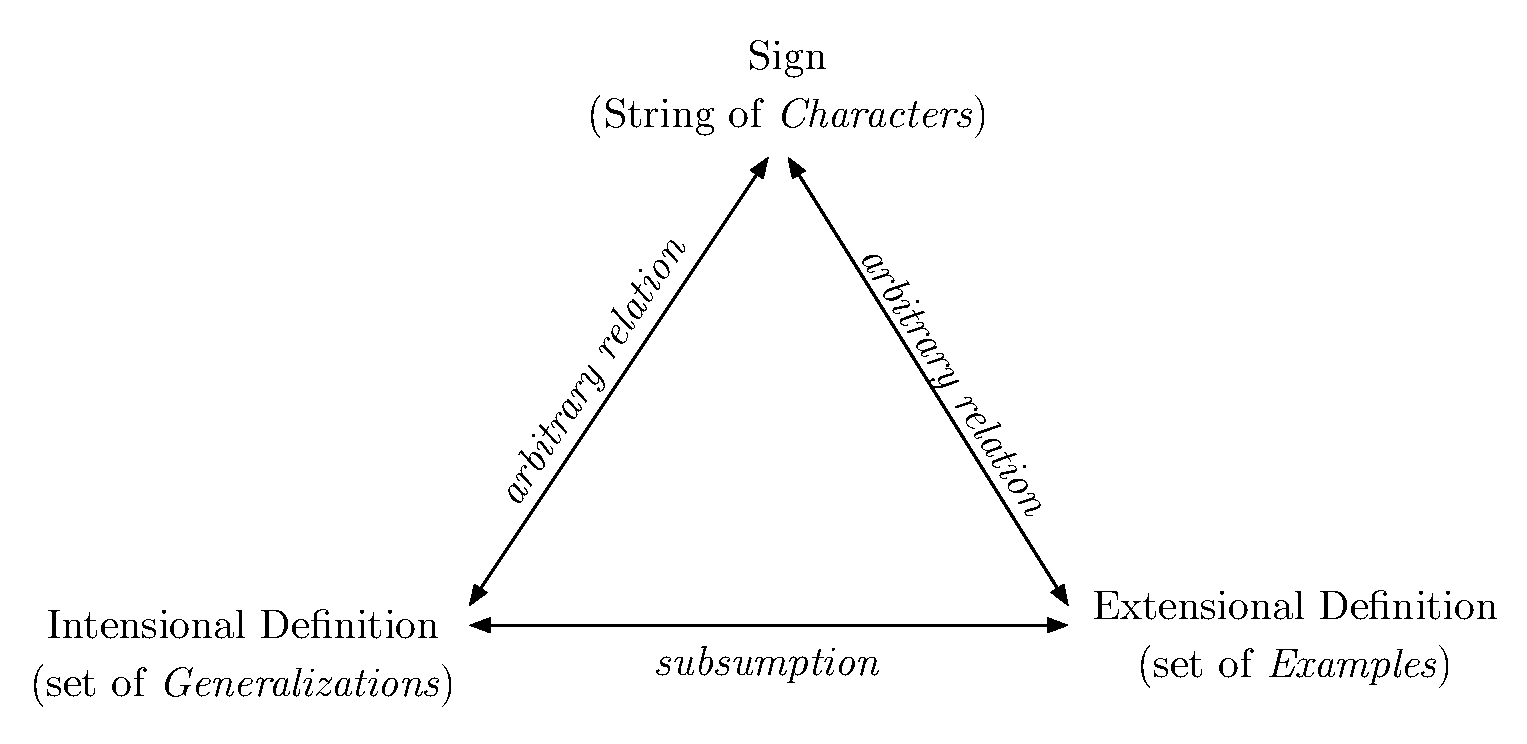
\includegraphics[width = \textwidth]{figs/4.pdf}
    \caption{The semiotic triangle and its elements}
    \label{fig:semTriangle}
\end{figure}

\section{Example-sign association}
% Presentation of the agents as inductive learner
The central element of the naming game and by extension of the classifier alignment is the example-sign association. While there are multiple ways to associate signs with examples, the agents from my thesis are classifiers that are able of supervised learning and have two main ways to make these associations.

% Present supervised learning
In supervised learning, an agent $A_{k}$ receives a \emph{consistent} set of example-sign associations $U_{k} \prescript{}{o}{\mapsto} S_{k}$ from an oracle. These associations are memorized by $A_{k}$ in a set of example-sign associations $U_{k} \prescript{}{k}{\mapsto} S_{k}$. We say that the examples $U_{k}$ are the examples that the agents have knowledge over, and are called the \emph{local} context of the agent. Comparably, the signs $S$ that an agent has knowledge over is the \emph{local} lexicon of this agent. Prior to having any supervised learning, the agent can already make example sign associations over the examples $U_{k}$ by looking up its set of example-sign associations $U_{k} \prescript{}{k}{\mapsto} S_{k}$ which constitutes an index of received example-sign associations. However, $A_{k}$ cannot make new example-sign associations.

% How the supervised learning works
The supervised learning takes place by using each example $e$ from $U_{k}$ as an input and the sign $s$ associated to $e$ in $U_{k} \prescript{}{o}{\mapsto} S_{k}$ as an expected output. Once the supervised learning is done, the agent should have learned a set of generalizations such that, provided any example $e$ and any generalization $g$, any agent could say if $e$ can be associated to $g$. Each of the generalizations that are learned are associated to a sign $s \in S_{k}$. In my thesis, the agents are inductive learners that use the feature-term formalism. The association between an example $e$ and a generalization $g$ can be tested through the relation of subsumption $g \sqsubseteq e$. The associations between examples, signs and generalizations is summarized in Figure \ref{fig:semTriangle}.

% The semiotic triangle
If we incorporate the notion of generalization to the notion of class that was already incorporating a set of examples associated to a given sign, we have a concept. A concept is is a class and the generalizations that are associated to its examples and its sign. Concepts are often represented as semiotic triangles, with their set of generalizations called the intensional definition and their set of examples called their extensional definition.

% Present the result of supervised learning (generalizations)
After the supervised learning, the agent $A_{k}$ can associate any example $e$ with a sign $s$ from its local lexicon through the generalizations that the agent has learned. First, the agents looks at which generalization $g$ is associated with the example $e$. Then, the agent looks at which sign $g$ is associated with. $A_{k}$ ends up with a new example-sign association. $A_{k}$ has now two ways of associating an example $e$ with a sign:

\begin{itemize}
    \item looking into $U_{k} \prescript{}{k}{\mapsto} S_{k}$ for an already existing example-sign association involving $e$.
    \item looking into $A_{k}$'s set of generalizations to find a generalization $g$ that subsumes $e$, and use the sign associated to $g$.
\end{itemize}

We call these two way of associating example with signs the left-path and the right-path associations, in reference to the path that they draw on the semiotic triangle that is presented in Figure \ref{fig:semTriangle}. The two paths are drawn in Figure \ref{fig:path}. We incorporate this distinction in the notation of example-sign association by adding the letter $l$ or $r$ for left path or right path the the usual notation $e \prescript{}{k}{\mapsto} s$. If the example $e$ is associated to the sign $s$ through the left path by agent $A_{k}$, we note $e \prescript{l}{k}{\mapsto} s$. On the contrary, if the example $e$ is associated to the sign $s$ through the right path by agent $A_{k}$, we note $e \prescript{r}{k}{\mapsto} s$. An accurate supervised learning results in  $U_{k} \prescript{r}{o}{\mapsto} S_{k}$ being the same set of associations as $U_{k} \prescript{l}{o}{\mapsto} S_{k}$.

\begin{figure}[t]
    \centering
    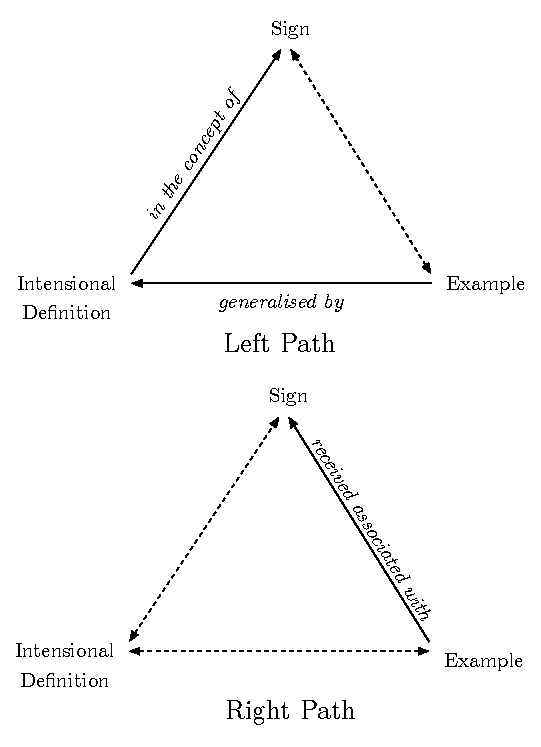
\includegraphics[width = 200pt]{figs/paths.pdf}
    \caption{Paths of example-sign associations offered to the agents. The right path is considered as the "objective truth" as it has been received by the oracle, while the left path is an inference made through learning that can be used in a more diverse set of scenarios to make new associations.}
    \label{fig:path}
\end{figure}

% Oracle distribution
In the case of a two-agents alignment scenario, the oracle can give different set of example signs associations for the agents to learn over. From now, I will consider that the general case is indeed $U_{k} \prescript{}{o}{\mapsto} S_{k} \neq U_{-k} \prescript{}{o}{\mapsto} S_{-k}$. The differences between $U_{k} \prescript{}{o}{\mapsto} S_{k}$ and $U_{-k} \prescript{}{o}{\mapsto} S_{-k}$ are responsible for most of the issues that are present in classifier alignment. Note that we keep using the notation  $U_{k} \prescript{}{o}{\mapsto} S_{k}$ for the set of associations received from the oracle, since the oracle does not use paths to make these associations. On the contrary, the generic set of received associations of $A_{k}$ is noted $U_{k} \prescript{r}{k}{\mapsto} S_{k}$ since all these associations are indeed right-path associations when they are made by $A_{k}$.

% Definition of homogeneity
The notions of left-path associations and right-path associations gives a better presentation of the role of learning and allows us to define the homogeneity of a set properly. As mentioned before, this definition is presented below:

\begin{restatable}[Homogeneity]{df}{Homogeneity}
\label{def:Homogeneity}
Let $A_{1}$ and $A_{2}$ be two agents. A set of example-sign associations $U \mapsto S$ is considered as homogeneous if, for any pair of its subsets $U_{1} \mapsto S$ and $U_{2}\mapsto S$ such that $(U_{1} \mapsto S) \cup (U_{2} \mapsto S)$, we have $U_{k} \prescript{l}{A1}{\mapsto} S = U_{k} \prescript{l}{A2}{\mapsto} S$.
\end{restatable}

Of course, a learning can be non-deterministic and often admits a degree of error, this is why we prefer to speak about a degree of homogeneity instead of a strict homogeneity. The degree of homogeneity is defined below:

\begin{restatable}[Degree of homogeneity]{df}{DoHomogeneity}
Let $A_{1}$ and $A_{2}$ be two agents. The degree of homogeneity $d_{h}$ of two sets of example-sign associations $U_{1} \mapsto S$ and $U_{2} \mapsto S$ is given by the formula:

\[
d_{h} = \frac{1}{2} \sum_{k = 1}^{2} \frac{|U_{k} \prescript{l}{A1}{\mapsto} S \cap U_{k} \prescript{l}{A2}{\mapsto} S|}{|U_{k} \mapsto S|}
\]

\end{restatable}

\section{Issues in Classifier alignment}

\subsection{Predictable issues in classifier alignment}
% Predictable issues linked to classifier alignment
The initial situation in which two classifier agents receive different sets of associations and learned over them. The possible differences between the result of this learning on the knowledge of these agents and the final state expected from these agents in order to have a classifier alignment allows us to make predictions on the issues that are linked to classifier alignment. While we have already mentioned that the general case is $U_{k} \prescript{}{o}{\mapsto} S_{k} \neq U_{-k} \prescript{}{o}{\mapsto} S_{-k}$, the types of differences between these two sets of associations allow us to classify the issues in alignment into main families, that we call situations of alignment.

% Agents might not share their examples
\paragraph{Different examples distributed:} The two sets of associations distributed by the oracle can be different simply because the examples that the agents receive are different. In this case, $U_{k} \neq U_{-k}$. The main issue associated with this case, is that the agents cannot use the right-path to associate a sign to the examples of the other agent since the examples from $U_{-k} - U_{k}$ are not found in $U_{k} \prescript{}{o}{\mapsto} S_{k}$. A more problematic issue is that it becomes hard to compare the classifications of the two agents, since their partitions are not the same: the class $U(\prescript{l}{k}{\mapsto} s)$ is likely to have different examples from the class $U(\prescript{l}{-k}{\mapsto} s')$ with both classes having their own particular examples. While this issue does not affect a naming game that uses the left-path to associate signs with presented examples, we will see later that this issue has a real impact when we will have to define a notion of equivalences between the concepts of different agents. Unfortunately, this case is the general case in machine learning and multi-agent systems, and is the only case considered in thesis. In the rest of the thesis, the sets of examples $U_{-k} - U_{k}$ and $U_{k} - U_{-k}$ are always non-empty, granting each agents with their own separate knowledge.

% Agents might not share their signs
\paragraph{Different signs distributed:} The two sets of associations distributed by the oracle can also be different because the signs that the agents received are different. In this case, $S_{k} \neq S_{-k}$. The main issue associated with this case is that even if two classes $U(\prescript{l}{k}{\mapsto} s)$ and $U(\prescript{l}{-k}{\mapsto} s')$ are equal, the agents will associate a different signs to their example and while the agents are sharing the partition of their examples, they are unable to pass the naming game.

% Agents might not share their example signs associations
\paragraph{Distinct example-signs associations} The two sets of associations are distributed by the oracle can share the same examples and the same signs, but still have different example-sign associations. In this case,  $U_{k} = U_{-k}$ and $S_{k} = S_{-k}$, but $U_{k} \prescript{}{o}{\mapsto} S_{k} \neq U_{-k} \prescript{}{o}{\mapsto} S_{-k}$. In the previously discussed cases, we could always imagine that there were one set of associations $U \prescript{}{o}{\mapsto} S$ that was distributed among the agents -- not the same associations in the case of the different examples distributed, and by substituting the signs of some classes in the case of different signs distributed, but we could always track the two sets distributed back to one set of associations that had classes. In the present case, it would be impossible without associating more than one sign associated to some examples. This case is better understood as if the oracle was distributing two distinct sets of associations instead of one to the classifier agents.

% Agents might not have their two paths making the same associations locally
\paragraph{Distinct local-path associations} The two agents have received the same set of associations and $U_{1} \prescript{}{o}{\mapsto} S_{1} = U_{2} \prescript{}{o}{\mapsto} S_{2}$. However, at least one of the agent $A_{k}$ did not succeed to make an accurate learning over the set $U_{k} \prescript{}{o}{\mapsto} S_{k}$. The consequence is that $U_{k} \prescript{l}{k}{\mapsto} S_{k} \neq U_{k} \prescript{r}{k}{\mapsto} S_{k}$. If the agents use the right path to name the examples that are presented to them during the naming game, this case is without incidence. However, if the agents use the left path to name the examples -- and we have already shown that the left-path should be the preferred path to make associations -- the agents will probably produce some errors. Indeed, a situation where the learning errors of $A_{k}$ and $A_{-k}$ are nullifying each others such that $U_{1} \prescript{l}{k}{\mapsto} S_{1} = U_{2} \prescript{l}{-k}{\mapsto} S_{2}$ is highly unlikely to happen.

% Agents might not associate one sign to one example
\paragraph{Unknown association and Multiple associations} Depending on the algorithm used for the supervised learning, an agent $A_{k}$ can end up with either none or more than one sign associated to one example - either an example from its local context $U_{k}$ in the case of an inaccurate learning, or an example presented later during the naming game, or an example exchanged with the agent $A_{-k}$. This can be the case in my thesis, since I use inductive learning and cannot guarantee that only one of the generalizations that come as the output of my learning are subsuming disjoint sets of examples in any context -- or that for any possible example, one of the learned generalization will subsume it.


\subsection{Classes of alignment situations}

% Presenting the issue with the combination of different cases
The issues that are listed in the previous section are not all mutually exclusive, and often a situation combines two or more of them. Even for mutually exclusive cases, some aspects of a case can be combined with some aspects of another in order to create a hybrid case. In my scenarios for instance, the examples that are received by the agents as learning sets are always at least partially different. What differentiates my scenarios are the other cases that are combined with the \emph{different examples distributed} case. As a direct consequence of this, the fact that the agents are not receiving the same examples at the beginning often masks issues that would have been better understood if they had received the same examples. For this reason, we need to look at these issues from the point of view of the oracle, and see how these issues are perceived by the agents after the distribution.

% Distinguish cases due to the learning and cases independent from the learning
Looking at the five cases of predictable issues listed in the section above, we can see that the three first cases of issues are independent of the agent's learning while the two lasts are caused by the learning inaccuracies or intrinsic limitations. In this section, we will see that it is sometime complicated to identify if a situation that causes issues in the classifiers alignment is due to the agents' learning or if the problem is totally independent. This information is however essential for the agents: an issue caused by an error in the learning can be corrected with the agents sharing their knowledge and learning again a more accurate set of generalizations. However, if the issue is not caused by the learning, the agents will need to question the nature of the information they have in order to overcome their disagreements.

\begin{figure}[t]
    \centering
    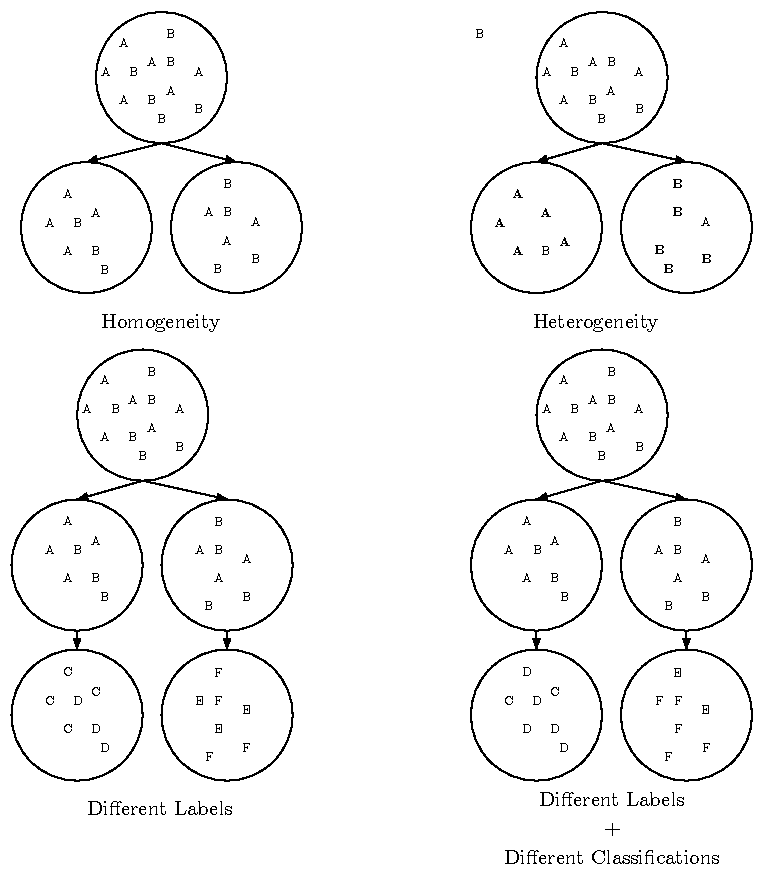
\includegraphics[width = 250pt]{figs/different_situations.pdf}
    \caption{The different situations of classifier alignments. The top circle always represent the hypothetical set of associations that the oracle is supposed to have access to. The letters represent the examples and their associated signs. The oracle's set of associations is either directly distributed among the agents (top line), or they go through a step of distribution and a state of alteration of the classes (bottom line).}
    \label{fig:classProblem}
\end{figure}

% Introduction to situations
The different combinations of cases, called situations, are presented below. In each situation, the local contexts $U_{1}$ and $U_{2}$ are different. Of course, situations can be combined as well in order to make hybrid situations. The situations are illustrated in Figure \ref{fig:classProblem}, and will be presented below as they appear on this figure from left to right.

% Homogeneity situation
\subsubsection{Homogeneity situation} The situation is homogeneous when the oracle has a unique and consistent set of associations $U \prescript{}{o}{\mapsto} S$ and gives to $A_{1}$ and $A_{2}$ different subsets of $U \prescript{}{o}{\mapsto} S$. In this scenario, the subsets receive associations from each class of $U \prescript{}{o}{\mapsto} S$ in similar proportion, which facilitates the classifier alignment. Indeed, the generalizations that will be learned over sets of examples of similar sizes are likely to be similar themselves, and we can expect to have $U \prescript{l}{A1}{\mapsto} S \approx U \prescript{l}{A2}{\mapsto} S$. Therefore, we can expect to observe a high score from $A_{1}$ and $A_{2}$ on a naming game that takes place over the context $U$, or even different contexts. The homogeneity is the most ideal distribution of examples that can take place in a situation where $U_{1} \prescript{}{o}{\mapsto} S \neq U_{2} \prescript{}{o}{\mapsto} S$.

% Heterogeneity situation
\subsubsection{Heterogeneity situation} The situation is heterogeneous when the oracle still has a unique and consistent set of associations $U \prescript{}{o}{\mapsto} S$ and gives to $A_{1}$ and $A_{2}$ different subsets of $U \prescript{}{o}{\mapsto} S$, but this time the agents receive associations from the classes of $U \prescript{}{o}{\mapsto} S$ in different proportions. The issue here is that the generalizations are likely to be different from one agent to another, even for a same classes, due to a lack of precision for the agent that has received the least examples of that class. Even if $U_{1} \prescript{l}{A1}{\mapsto} S \approx U_{1} \prescript{r}{A1}{\mapsto} S$ and $U_{2} \prescript{l}{A2}{\mapsto} S \approx U_{2} \prescript{r}{A2}{\mapsto} S$, the difference in composition between $U_{1}$ and $U_{2}$ are likely to cause $U \prescript{l}{A1}{\mapsto} S \neq U \prescript{l}{A2}{\mapsto} S$.

% Different signs situation
\subsubsection{Different signs situation} The situation of different signs is also based on the case of different examples distributed, but this time mixed with the case of different signs distributed. As for the situations of homogeneity and heterogeneity, we can imagine the oracle distributing the associations of a consistent set of associations $U \prescript{}{o}{\mapsto} S$ between two sets of associations, $U_{1} \prescript{}{o}{\mapsto} S$ and $U_{2} \prescript{}{o}{\mapsto} S$. However this time, before giving these sets of associations to the two agents, the oracle is replacing the lexicon $S$ of these sets by two new separate lexicons $S_{1}$ and $S_{2}$. In this situation, the classes are not modified: if the sign $s \in S$ has been replaced by the sign $s_{k} \in S_{k}$, we observe the equality $U(\prescript{}{o}{\mapsto} s) = U(\prescript{}{o}{\mapsto} s_{k})$. The fact that $U_{1}(\prescript{}{o}{\mapsto} s_{1}) \neq U_{2}(\prescript{}{o}{\mapsto} s_{2})$ is imputable to $U_{1} \neq U_{2}$, not to $S_{1} \neq S_{2}$. In this situation, the set of associations $(U_{1} \prescript{}{o}{\mapsto} S_{1}) \cup (U_{2} \prescript{}{o}{\mapsto} S_{2})$ is not consistent, but each of its example is associated with exactly one pair of signs: one sign from $S_{1}$ and one sign for $S_{2}$. Additionally , if an example from the set $(U_{1} \prescript{}{o}{\mapsto} S_{1}) \cup (U_{2} \prescript{}{o}{\mapsto} S_{2})$ is associated with two signs $s_{i} \in S_{k}$ and $s_{j} \in S_{-k}$, then there cannot be another example $e'$ from the same set associated to a pair of signs $s_{i} \in S_{k}$ and $s_{l}' \in S_{-k}$ such that $s_{j} \neq s_{l}$.

% Different classifications situation
\subsubsection{Different classifications situation} The situation of different classifications is base on the case of different examples distributed. In this situation, the union $U_{1} \prescript{}{o}{\mapsto} S_{1} \cup U_{2} \prescript{}{o}{\mapsto} S_{2}$ does not form a consistent set of consistent example-sign associations. While this was also the case in the situation of different signs, this time there is no relation of equivalence between the classes of $U_{1} \prescript{}{o}{\mapsto} S_{1}$ and $U_{2} \prescript{}{o}{\mapsto} S_{2}$. In this situation there can be an example from the set $(U_{1} \prescript{}{o}{\mapsto} S_{1}) \cup (U_{2} \prescript{}{o}{\mapsto} S_{2})$ that is associated with two signs $s_{i} \in S_{k}$ and $s_{j} \in S_{-k}$, and a second example $e'$ that is associated with another pair of signs $s_{i} \in S_{k}, s_{l} \in S_{-k}$ such that $s_{j} \neq s_{k}$. Intuitively, it does not seem that this situation can be explained as the distribution of a consistent set of associations, but rather as the oracle presenting two unrelated sets of associations to the agents. However, we can imagine that there exists a consistent set of associations $U \prescript{}{o}{\mapsto} S$ that has been distributed in two subsets $U_{1} \prescript{}{o}{\mapsto} S$ and $U_{2} \prescript{}{o}{\mapsto} S$ such that $U_{1} \neq U_{2}$, that are therefore consistent as well -- so far, this in an homogeneous situation. In order to explain how two examples that belong to a same class in $U_{k} \prescript{}{o}{\mapsto} S_{k}$ can belong to two different classes in  $U_{-k} \prescript{}{o}{\mapsto} S_{-k}$, we can imagine that some of the classes from one set $U_{k} \prescript{}{o}{\mapsto} S_{k}$ has been merged together. A merge between two classes $U(\prescript{}{o}{\mapsto} s_{i})$ and $U(\prescript{}{o}{\mapsto} s_{j})$ of the set of associations $U_{k} \prescript{}{o}{\mapsto} S_{k}$ is done by removing the set of associations of the two classes, $U(\prescript{}{o}{\mapsto} s_{i}) \prescript{}{o}{\mapsto} s_{i}$ and $U(\prescript{}{o}{\mapsto} s_{j}) \prescript{}{o}{\mapsto} s_{j}$, and replacing them by a new set of associations $(U(\prescript{}{o}{\mapsto} s_{i}) \cup U(\prescript{}{o}{\mapsto} s_{j})) \prescript{}{o}{\mapsto} s_{l}$ that associates the union of the two classes merged to a same sign $s_{l}$. Since the number of classes changes each time that a merge occurs, the sizes of the lexicons change as well as they become different. Then, the resulting sets of associations are given to the agents as $U_{1} \prescript{}{o}{\mapsto} S_{1}$ and $U_{2} \prescript{}{o}{\mapsto} S_{2}$.

\section{Reaching Mutual Intelligibility}

% Introduction
The details of our approach to reach mutual intelligibility will be addressed later in the thesis, with the proper notation. However, we can already discuss generalities on how multi-agent systems can align themselves.
% Alignment is in fact left path alignment
The first thing that should be decided over the alignment, is if we want a left-path or a right-path alignment, or a mix of the two. Indeed, the agents have two different paths to associate a sign with an example and therefore can name a presented example with more than one path on certain conditions. The problem is that these paths, as we mentioned before, might not make the same associations. Therefore, the first thing that an agent should know in order to play the naming game is which path should be used when. While the right-path represent a knowledge obtained from the oracle and therefore deemed as more accurate, the right-path can only help to name examples that are part of the examples received from the oracle. This limitation forces the agent to prefer the left-path for most of the examples involved in the naming game. Of course, an agent could use the right-path by default and resort to the left-path only for examples that it has not receive from the oracle, but mixing paths in the naming game can be problematic: for instance, in the case of agents arguing, there is a risk that an agent names an example with a sign that seems inconsistent with the generalizations and arguments that this agent has shared with the other agent. We call this left-path alignment \emph{mutual intelligibility}.

\subsection{Reaching mutual intelligibility according to the situation}

\subsubsection{Homogeneity and heterogeneity} The situation of homogeneity should not cause any problem and the classifiers should already be quasi-aligned after the supervised learning. The situation of heterogeneity is close to the one of homogeneity, but induces more overlaps between the left-path associations of the two agents. We can in fact consider that a situation of homogeneity becomes a situation of heterogeneity not when a threshold is reached in the imbalance of examples between classes of the two agents, but when the left-path associations of the two agents are resulting in too many errors during the naming game for the agents to consider that their learning data-sets where homogeneous. In these two situations, the agents could just exchange all of their example-sign associations to find the original set of associations $U \prescript{}{o}{\mapsto} S$ that is the union of their two local sets. With this overall set of associations, the agent could learn new generalizations for their left-path associations without difficulty, since as we mentioned the overall set of associations is consistent. Of course, transferring all the examples from one agent to another is costly in term of information exchanged examples. This is were algorithms such as Amail intervene: they use arguments that summarize the information of chosen subsets of the local sets of associations, and allow the agents to reduce the volume of information that they need to exchange in order to align their left-path associations.

\subsubsection{Different signs} The situation of different signs is radically different the the homogeneity and heterogeneity situation. An algorithm like Amail could not directly be used in this situations, since the union of the two local sets of example-sign associations of the agents is not a consistent set of associations. Therefore, it cannot be used as a learning set for supervised learning by the agents. This means that even if the agents were to exchange all of their example-sign associations, they could not anything that would help them to pass the naming game. However, since the classes of the agents are mapped one to one, the agents can make a pre-processing \emph{before} using Amail.
% The mapping
In this pre-processing, the agents will find correspondences between their classes by examining which of them are equivalent. Of course, since the agents have different examples, the classes from different agents are almost always expected to be different -- it is the case in any scenario. However, the agents can look at the equivalence in the overall context $U_{1} \cup U_{2}$, by finding the pairs of classes $(U_{1} \cup U_{2}) \prescript{l}{A1}{s_{i}}$, $(U_{1} \cup U_{2}) \prescript{l}{A2}{s_{j}}$ are having the same examples. We call this process a \emph{mapping} of the classes of the two agent. The agents can do this mapping by exchanging all of their examples to have both access to the overall context, but if they want to limit the amount of information exchanged they can use ontology matching algorithms in order to make a one-to-one mapping of their classes.
% From mapping to a situation of homogeneity or heterogeneity
Once the classes are mapped, the agents can change the signs associated to the examples of these classes -- that should be two different signs per matching classes, one from each agent's lexicon -- to a common sign per matching classes. Once this is done, the agents are finally using the same lexicon. The union of the two agents' sets of associations is now a consistent set, and the agents are in a situation of homogeneity or heterogeneity on which algorithms like Amail can make the agents reach mutual intelligibility.

\begin{figure}
    \centering
    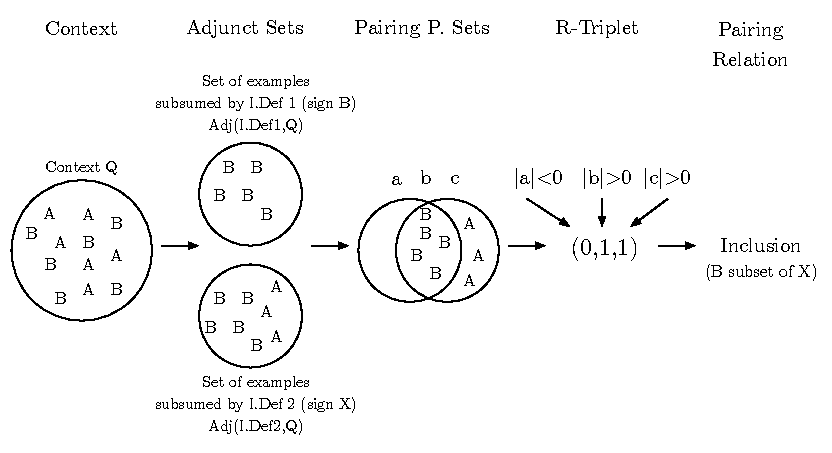
\includegraphics[width = 250pt]{figs/5.pdf}
    \caption{Relation between the context, concepts' adjunct sets, pairing partial sets, r-triplets and pairing relations. The left-path (intensional definitions) partitions a context into adjunct sets. Two adjunct sets create three theoretical pairing partial sets. The count of examples in each pairing partial sets gives the r-triplet of the relation between the two adjunct sets. The r-triplet gives the quality of the pairing relation of the concepts from with the left-paths have been borrowed to make adjunct sets.}
    \label{fig:pRelations}
\end{figure}

\subsubsection{Different classifications} The situation of different classifications is comparable to the situation of different signs in the sense that the union of the two local set of associations of the agents cannot make a consistent contrast-set. However, unlike the situation of different signs, there is no possible one-to-one mapping between the classes of the agents and this is why there is no pre-processing that can turn this situation into something compatible with Amail without seriously altering the classes of both agents, as learning and argumentation is only useful if the agents are learning and arguing within an overall set of relations that is consistent. There can be two approaches to overcome this problem.
% How did we get there
We mentioned that this situation is analog to an oracle distributing the associations of a consistent set of associations $U \prescript{}{o}{\mapsto} S$ among two subsets $U_{1} \prescript{}{o}{\mapsto} S$ and $U_{2} \prescript{}{o}{\mapsto} S$, and then merge differently the classes of each of these two sets in order to obtain two new sets $U_{1} \prescript{}{o}{\mapsto} S_{1}$ and $U_{2} \prescript{}{o}{\mapsto} S_{2}$.
% Create a mapping
After the merge, it is impossible for the agents to make a one to one mapping of their class since they might even differ in number from one agent to another. Instead of doing a one-to-one mapping based on a relation of equivalence between the classes, the agents can do a all-to-all mapping using \emph{pairing relations}. Unlike the relation of equivalence that can only map two classes $(U_{1} \cup U_{2}) \prescript{l}{A1}{s_{i}}$ and $(U_{1} \cup U_{2}) \prescript{l}{A2}{s_{j}}$ if they have the same examples, the pairing relations can map these two classes no matter how many examples they have in common. The information about these classes having examples in common is stocked as r-triplets. The relation between pairing relations, r-triplet and the sets of examples shared by the two classes (called pairing partial sets) is presented in Figure \ref{fig:pRelations}. As Amail was useful to spare information transfer in situations of heterogeneity, and ontology-matching algorithms were useful to spare information transfer in situations of different signs, the argumentation model that I propose comes with a process that spares information in the different classifications situations when it comes to identify the pairing partial sets, r-triplets and pairing relations of the agents.
% Reverse the merge
Once the mapping is done, the agents have all the information they need to identify the classes that have been merged in $U_{1} \prescript{}{o}{\mapsto} S$ and $U_{2} \prescript{}{o}{\mapsto} S$. By splitting their classes, the agents can reverse the process of merging that theoretically occurred in the two sets $U_{1} \prescript{}{o}{\mapsto} S$ and $U_{2} \prescript{}{o}{\mapsto} S$. The splits result in a class for each pairing partial set that were present in the mapping; a pairing partial set can also be seen as a class $(U_{1} \cup U_{2})(\prescript{l}{k}{\mapsto} s_{i},s_{j})$ of the union of the two local sets of associations. Therefore, there will be a new class for each different pair of signs that can be find in the union of the two local sets of associations.
% Make a one to one mapping
Once the split has been done, the agents have a new set of classes. Since there is a new class for each pair of signs that are associated to examples in the union of the two sets of associations, the agents can now make a one to one mapping of their classes. The agents have reached a situation of different signs. The agents can, by using an ontology alignment algorithm, reach a situation of heterogeneity or homogeneity.
% Again, we are in a situation where we can use Amail
Once in a situation of heterogeneity or homogeneity, the Amail algorithm can be use to reach mutual intelligibility over the overall context of the agents.

\subsection{Identifying the Situation}

In the previous section, we have detailed how to move from each situation to a situation of homogeneity where the agents share enough information to learn intensional definitions that are allowing mutual intelligibility. The path followed through the simplification of these situations is illustrated in Figure \ref{fig:simplification}.

\begin{figure}
    \centering
    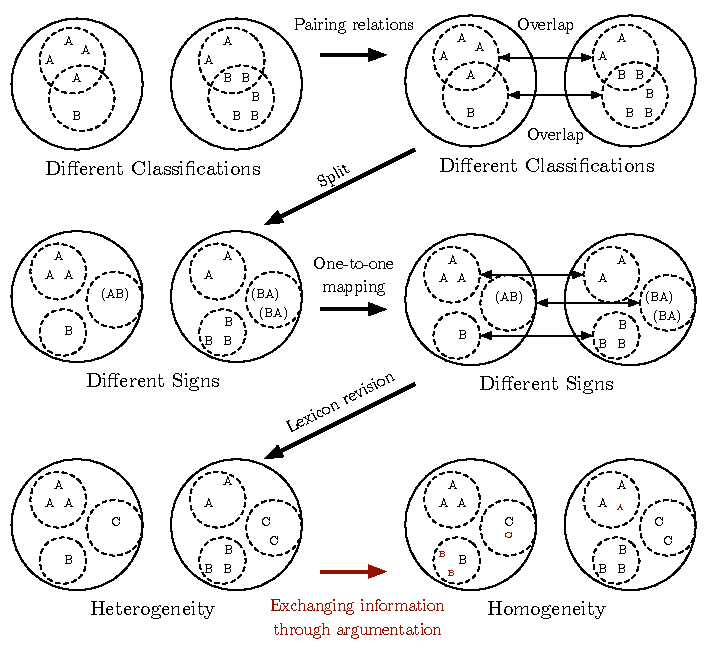
\includegraphics[width = 250pt]{figs/situations_simplification.pdf}
    \caption{The simplification of each situation into a simpler one, each time presented with the method used.}
    \label{fig:simplification}
\end{figure}

However, the agents have no \emph{a priori} knowledge on which scenario they are when they meet each other and try to reach mutual intelligibility. Therefore, before using any method to simplify their current situation they need to figure out which is their actual current situation.

% Why we are in a different paradigm when we try to solve and when we try to identify a situation
The problem with the identification of the situations, is that we are classifying them according to a narrative that is just an abstract justification for the differences between the agents' classifications. This narrative of an oracle that distributes the examples of a consistent set of associations among two subsets might or might not have a reality in our scenarios, as the experimenter might follow these steps to create the training set of the examples or use two already-different training sets. In the latter scenario, we can always imagine that the two already-different training sets are parts of a reality that can be seen as a consistent set of associations, if we chose to put ourselves in a constructivist paradigm. However, all these steps are hypothetical and we only presented them to produce a reverse model of this narrative that leads to a consistent set of associations where there are actually two sets that seems to contain at least some inconsistent information. While understanding this idea is important to present how to reach mutual intelligibility in each different situation, it has no use to try to guess in which situation are the agents.

% Since we cannot access the narration that led to the creation of these two sets, we should look at the effect that this narration has
The narration of the situation's creation is hypothetical, and even in cases where it is not, the agents cannot directly access it. Therefore, the identification of the different solutions requires to look for the effects of this narration over the sets of associations of the agents.

%% Effect on the right path associations
\subsubsection{Effect on the right-path associations}

\begin{figure}
    \centering
    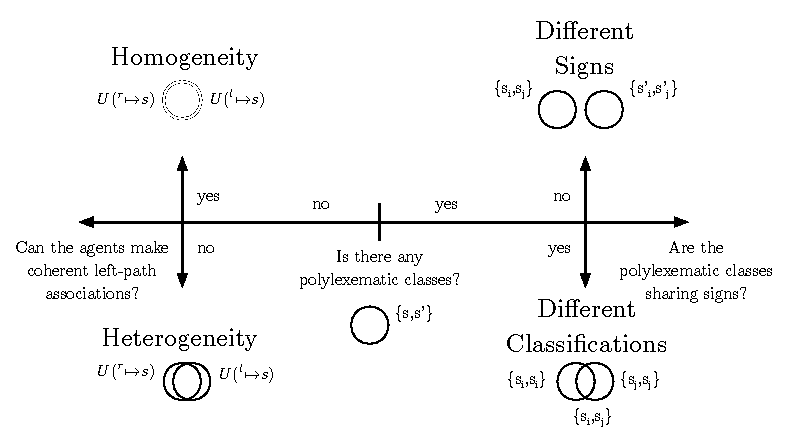
\includegraphics[width = \textwidth]{figs/situations_id_r.pdf}
    \caption{Identification of the agents' situation based on right-path associations comparison.}
    \label{fig:r_situation_id}
\end{figure}

% The creation of situations affects primarily the right path associations
The creation of the local training sets of associations is only involving the right-path associations, since the associations given by the oracle to the agents at the start of any scenario are treated as right-path associations.
% Can check the presence of polylexematic classes
Identifying the situation is trivial if the agents have access to both $(U_{1} \cup U_{2}) \prescript{r}{A1}{\mapsto} S_{1}$ and $(U_{1} \cup U_{2}) \prescript{r}{A2}{\mapsto} S_{2}$. The agents are by definition in a situation of homogeneity or heterogeneity if and only if the union of these two local sets of associations are consistent. This verification splits the situations in two classes, that we will call consistent and inconsistent situations. The consistent situations are the homogeneity and heterogeneity situations, while the inconsistent situations are the different signs and different associations situations. Once the agents have determined if the situation is consistent or inconsistent by checking the union of their local sets of associations, they can determine for each class which of the two situations inside is their current situation.

% homogeneity vs heterogeneity
If the agents determined that their situation is a consistent relation, they can use their supervised learning over their respective local sets of associations to see if they obtain the same generalizations. If this is the case, then the information has been homogeneously distributed between their training sets and they are in a homogeneous situation. On the contrary, if the generalizations over the two local training sets classify the other agent's training set with differences compared to the right-path associations, the agents know that they are in a situation of heterogeneity.

% different signs vs classifications
If the agents have found polylexematic classes in the union of their local training sets, they know that they are either in a situation of different signs or different classifications. By looking at the different set of signs associated to each of the classes, the agents can determine in which situation they are. There can exist two classes $(U_{1} \cup U_{2})(\prescript{r}{}{\mapsto} \{s_{i},s_{j}\})$ and  $(U_{1} \cup U_{2})(\prescript{r}{}{\mapsto} \{s_{i}',s_{j}'\})$ such that $s_{i} = s_{i}'$ but $s_{j} \neq s_{j}'$, if and only if the agents are in a situation of different classifications. Therefore, there are no such pair of classes in the union of the two training sets, the agents know that they are in a situation of different signs.

% Problem with creating a set of right-path associations that can allow this identification
The problem with this identification method is that it requires the agents to create the set of associations $((U_{1} \cup U_{2}) \prescript{r}{A1}{\mapsto} S_{1})$ $\cup$ $((U_{1} \cup U_{2}) \prescript{r}{A2}{\mapsto} S_{2})$. A set of association $(U_{1} \cup U_{2}) \prescript{r}{k}{\mapsto} S_{k}$ can exist only if the agent $A_{k}$ has received it as its initial training set, or in other words if its initial training set contained all the examples from $U_{1}$ and $U_{2}$ -- which is the same as saying that $U_{1} = U_{2}$. Since this is a particular case, the agents are not able to use their right path associations to identify their situation in the general case.

%% Effect of the left path associations
\subsubsection{Effect on the left-path associations}

% Then the only option left is the left path associations
Since comparing the right-path associations of the agents has been ruled out, the agents can only compare their left-path associations if they want to determine their situation. In order to determine which are the effects of the distribution process over the different situations, we will take as a reference the homogeneous situation and consider the three other situations as variations. Then we can observe the effect of each variation on the differences between the left-path associations of the two agents.

% Ideal sets are homogeneous sets
The ideal sets are homogeneous. If the sets are homogeneous, the agents can substitute the 

% Each other situation is a deviation from the homogeneous situation

% The heterogeneous is (-) information shared

% The different signs is (-) lexicon shared

% The different classifications is (-) classes shared

% Each of the three deviations have the same impact: union of the two sets with polylexematic classes

\section{Argumentation and example exchanges}

\chapter{State of the Art}\label{StateOfTheArt}
% Introduction

\section{Introduction}

Binding the Introduction chapter with the plan of this state of the art.

\section{Knowledge Representation}

Presenting why knowledge representation is central in MAS, speak about heterogeneous data, the present challenges faced in Computer Sciences with Big Data, IoT, etc (see Paula)

\subsection{General Approaches of Knowledge Representation}

Really general introduction to knowledge representations, mostly to introduce the general dichotomy of grounder / connected meaning that we will find everywhere else

\subsubsection{Dictionary Approach}

Self explanatory. Since we are not focusing on this approach, we explain its limitations on the stuff that we want to do later: consistency of vocabularies, minimal number of concepts etc.

\subsubsection{Encyclopedic Approach}

Again, general presentation. Already linking it to the Connectivist approach on meaning.

\subsection{Knowledge Representation and Machine Learning}

Mainly to introduce the vocabulary and formalism used later in the text.

\subsubsection{Case-Based Reasoning}

Presenting CBR here, with opening on argumentation theory and work done with AMAIL.

\subsubsection{Symbol Grounding}

How to represent grounded meanings, FCG, etc

\subsubsection{Connectivism}

Continue the Encyclopedic approach in the introduction of contrast sets and related meanings

\subsection{Ontological Knowledge}

Still connected meaning, but more formalized and organized. Talk about the distinction between classes and categories, object oriented approach etc synthesis of encyclopedic and conectivist approach

\subsection{Cognitive Science}

The philosophical ground of out work

\subsubsection{Philosophy}

Wittgenstein, Pierce as situated meaning (language is its use)

\subsubsection{Ethology}

Presentation of Frake and the contrast set, relation with Ontology, Encyclopedic knowledge and connectivist approach of meaning, the contrast set as a unit of category and the concept as the unit of class.

\section{Communication}

Now that knowledge representation has been introduced, how agents can communicate about them

\subsection{Language Philosophy}

Introducing Saussure, linked to the connectivists, then speaking about semiotics but still introducing more general notions

\subsection{Information Theory}

Introducing Shannon and more generally computational take on communication, Pierce's adaptation and criticts (no context), the problem of semantic noise and how it is consistent with the notion of contrast sets

\section{Binding Knowledge Representation and Communication}

Restating the problematic of joining the constraints on KR and communication for agents.

\subsection{Ontology Matching}

Matching ontologies, problem: suppose an alignment on classes if not labels

\subsection{Argumentation Theory}

Arguing on concepts, problem: suppose an alignement of labels then match classes

\subsection{Semiotics}

How the triadic relations allows to map unmatching classes and labels


MOSTLY, THE JOB IS TO INTRODUCE A DISAMBIGUATION BETWEEN CONCEPTS LIKE "CLASSES \& CONCEPTS" OR "LABEL, SIGN, SYMBOL" etc

Agents are by definition taking actions in their environment. This requires that they are able to classify their stimuli (elements from their environment), their actions and the consequences of their action. This is often formalized as the input/output approach in ML. So Agents can be seen as classifiers.

Agents that use language are able to communicate with other agents on these classifications. They associate each class with a sign. Then they use the sign to access the different speech acts that allows language, but not our focus here. Problem: how to guarantee that the class-sign associations of two different agents are consistent, and what ``consistent'' means here?

First, how these classes are organized. They are organized in different category (if a class is a color, then a category is 'colors'). Explanation of how to build categories upon classes is given by -- give a synthesis of the state of the art -- and we pick the explanation of ethnography: the contrast set.

The contrast set gives a connexionist approach of the organization of categories, which is okay to define the interactions of classes between one category, but does not explain how to versions of a category belonging to two different agents can be consistent. For this, we take a look to semiotics, the science of signs and their relation with knowledge and reality. 

The present thesis focuses on a situation where two agents that {\color{red} learned their knowledge under different supervised learning? Or do we want to be more general? I remember that you didn't want to talk about learning. However, wouldn't it be helpful to present later the expected differences between the agent's knowledge that we formalize as contrast sets?}

% Communication

% Contrast sets

% Concepts

% Mutual Intelligibility

% Semantic alignement

% Ontology mapping

% Argumentation on the meaning

\chapter{Approach}\label{Approach}
\section{A Semiotic Approach of Agents and Communication}

\subsection{An Overview of Feature Terms}\label{sec:FT}

Our protocol of argumentation is based on the capacity of agents to associate a semiotic elements from any type with a given set of examples -- the adjunct set. While this capacity can be granted by various approaches in machine learning -- as long as they can be interpreted as generalizing over and classifying examples, we will mostly focus on the use of feature terms to associate the semiotic elements with their adjunct sets.

Feature terms, also called feature structures or $\psi$-terms, are a generalization of first-order terms that have been introduced in theoretical computer science in order to formalize object-oriented capabilities of declarative languages \cite{}. Feature terms correspond to a different subset of firs-order logic than description logic, but have the same expressive power \cite{}.

\begin{figure}\label{fig:TrainGraphic}
\centering
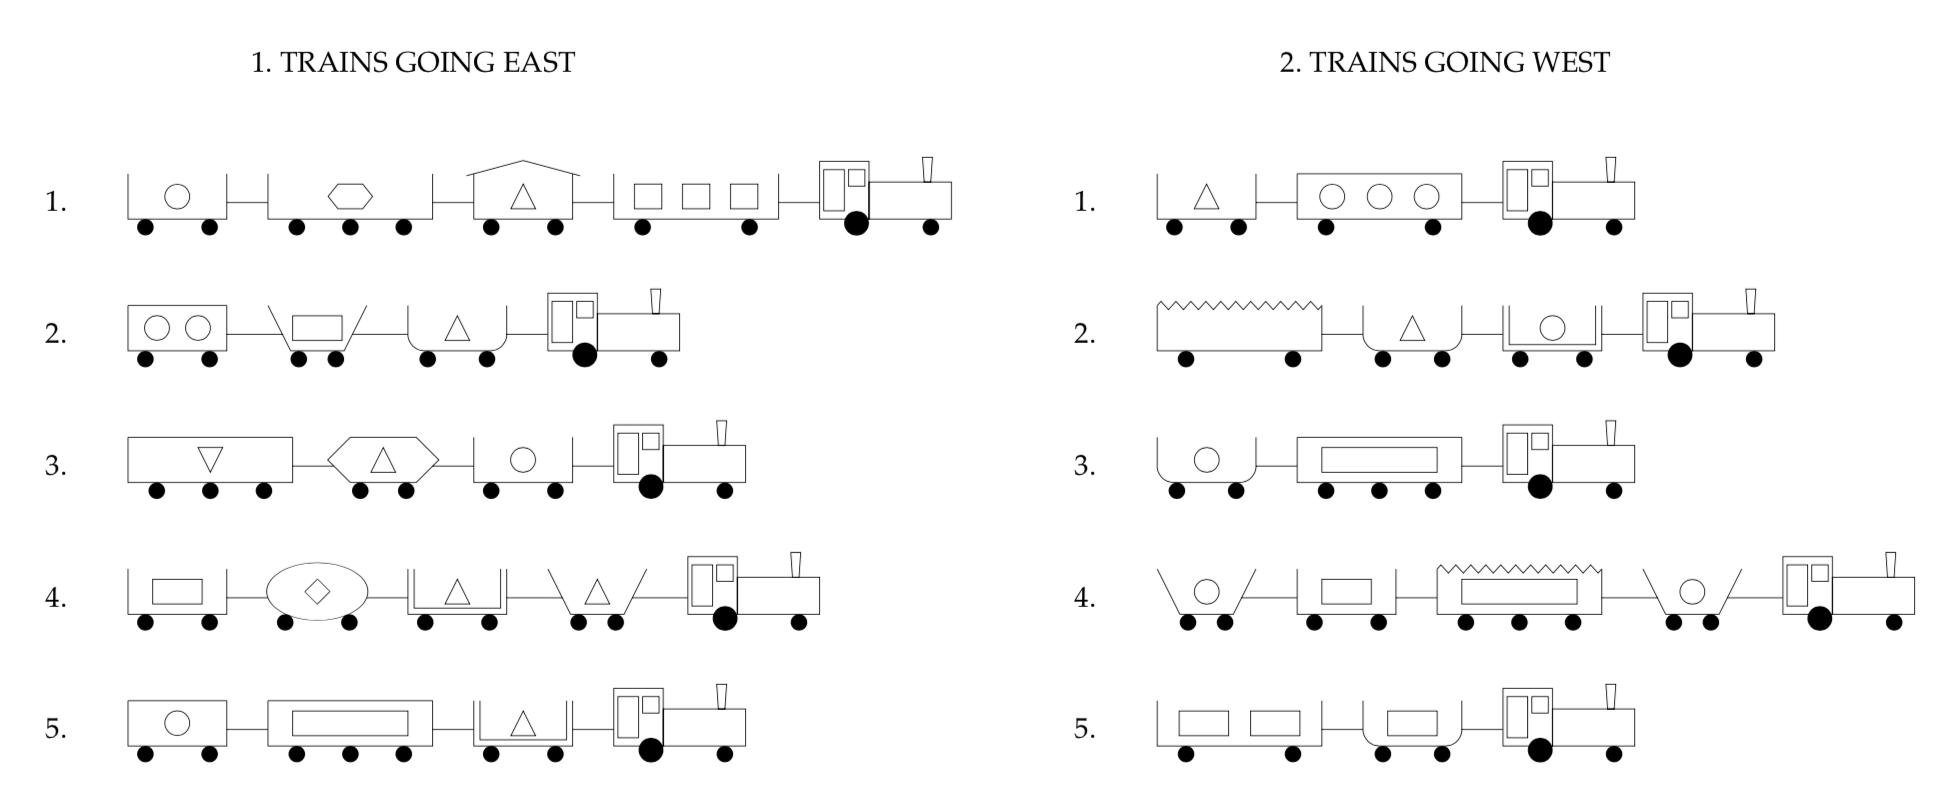
\includegraphics[width=\textwidth]{figs/trains}
\caption{Trains data set as introduced by Michalski.}
\end{figure}

The example of feature terms presented bellow is taken from the journal paper \textit{Similarity Measures over Refinement Graphs}  \cite{}. Consider the apparently simple Trains data set shown in Figure \ref{fig:TrainGraphic}, introduced by Michalski \cite{}: the original task is to learn the rule that discriminates east-bound from west-bound trains. If we were to represent such data set using a feature vector, we would need to define features for each one of the cars of a train (size, shape, load, and number of wheels), and determine beforehand a maximum number of cars per train (since feature vector representations have a fixed number of features).

Notice, however, that not all the trains have the same number of cars, and that, in principle, a train may have an unbounded number of cars. Thus, it is difficult to represent this data using a feature vector without losing information. Using a relational representation, we can just represent each car as a term, and define that a train is a set of cars, without restricting the number of cars of the train or the load each train is carrying.

\begin{figure}\label{fig:TrainFT}
\centering
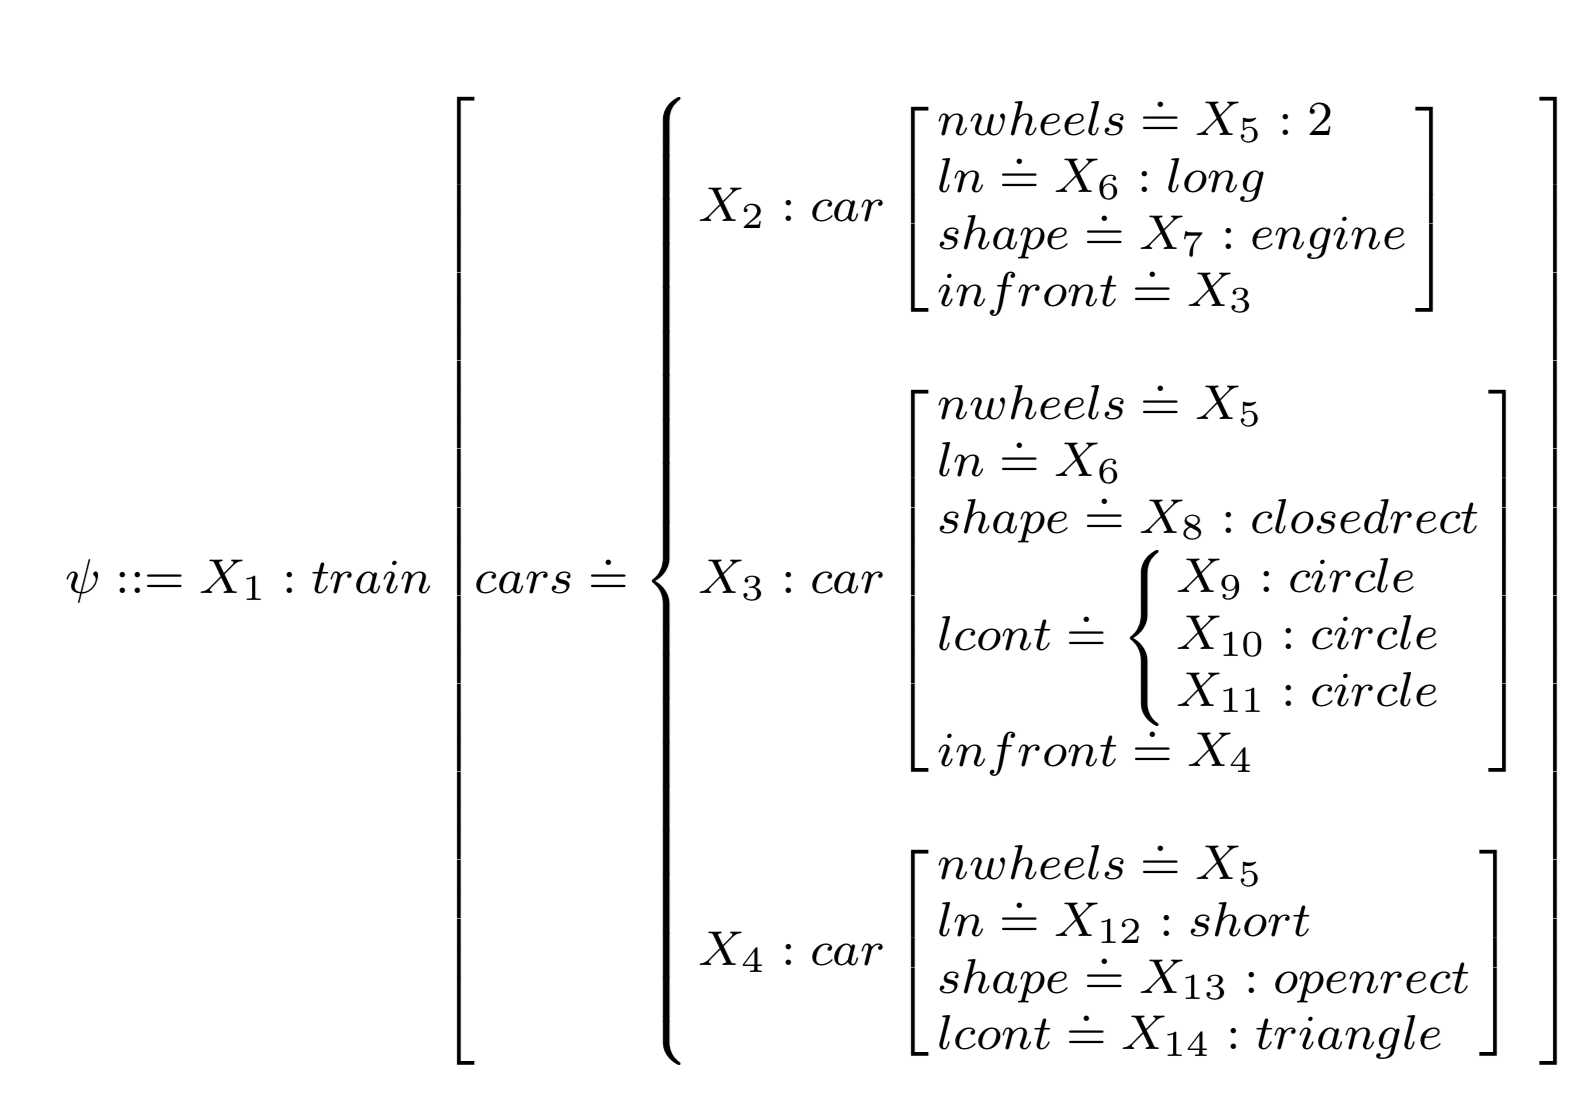
\includegraphics[scale = 0.4]{figs/trains3}
\caption{First west-bound train from Figure \ref{fig:TrainGraphic} represented in term notation.}
\end{figure}

On the other hand, Figure \ref{fig:TrainFT} represents the first west-bound train from Figure \ref{fig:TrainGraphic} using the feature term notation. We can see that the term is composed of 14 variables. The term contains two set- valued features (indicated by a curly bracket): in the feature cars of variable $X1$, and in the feature \emph{lcont} of variable $X3$. Finally, we can also see that there are several variable equalities in this term. Since the value of the feature \emph{infront} of variable $X2$ is the already defined variable $X3$, we note $X2.infront \doteq X3$, and also $X3.infront \doteq X4$. Additionally, the number of wheels in all the cars is the same, and the length of the first two cars is also the same.

The basic operation between feature terms is \emph{subsumption}: we will use $\psi_{1} \sqsubseteq \psi_{2}$ to express that a term $\psi_{1}$ subsumes another term $\psi_{2}$ – that is to say $\psi_{1}$ is more general (or equal) than $\psi_{2}$. Another interpretation of subsumption is that of an “informational content” order: $\psi_{1} \sqsubseteq \psi_{2}$ means that all the information in $\psi_{1}$ (all that is true for $\psi_{1}$) is also contained in $\psi_{2}$ (is also true for $\psi_{2}$)\footnote{In our work, we use the definition of subsumption introduced in \cite{} which has a slightly different definition than the traditional $\theta$-$subsumption$. Specifically, the difference is that we introduce the constraint that all the elements in a set have to be different.}.

\section{Concepts and Contrast Sets}\label{sec:Formalism}

\subsection{Semiotic Elements}\label{sec:SemEl}

The semiotic element are the components of concepts and containers. The different elements that an agent has perceived in its environment are called \emph{examples}. For example, a specific bird is an example of \emph{birds} or \emph{animals}. Birds and animals are two \emph{domains} in which we find birds. Domain is used here as a short for application domain.  Each example is identified by an index $i$ and noted $e_{i}$. Unless specified otherwise, agents are representing examples using a feature-term. A subset of a domain is a \emph{context}, the examples from the domain that a given agent has knowledge of, which we define in Definition \ref{def:Context}.

\begin{restatable}[Context]{df}{context}
\label{def:Context}
A context $U = \{ e_{1} \ldots e_{n} \}$ is a set of examples that covers a large part of a domain. 
\end{restatable}
A context needs to have enough examples to be partitioned into several non-empty sets.

An agent can classify the examples of a context into sets of examples called \emph{extensional definitions}. An extensional definition is associated to a specific category of the domain: for instance, the set of all birds of pray in a zoo can be an extensional definition for \emph{bird of prey} in the context of the zoo's aviary, for the domain of birds. Definition \ref{def:ExtD} formalizes this.

\begin{restatable}[Extensional Definition]{df}{extensional}
\label{def:ExtD}
An extensional definition is a non-empty subset of a context: $E_{i} \subset U$ and $E_{i} \neq \emptyset$. Extensional definitions are semiotic elements.
\end{restatable}

Some examples share similar features, and therefore can be generalized. A set of generalizations that generalize all the examples from an extensional definition is called an \emph{intensional definition} (see Def.\ref{def:IntD}). When the examples are represented as feature terms, the generalizations are also represented as feature terms that subsume sets of examples.

\begin{restatable}[Intensional Definition]{df}{intensional}
\label{def:IntD}
Let $X \subset U$ be a subset of examples of a context $U$, an intensional definition of $X$ is a set of generalizations $I_{i} = \{ g_{1}, \ldots , g_{n} \}$ such that $\forall e \in X, \exists g \in I_{i}$ such that $g \sqsubseteq e$, $\forall g \in I_{i}, \exists e \in X$ such that $g \sqsubseteq e$, and $\forall e' \in U-X, \nexists g \in I_{i}$ such that $g \sqsubseteq e'$. If an example $e$ is subsumed by a generalization from $I_{i}$, we note $I_{i} \sqsubseteq e$. Finally, we define as $X_{i} = \{ e \in U | I \sqsubseteq e \}$ the set of examples from $U$ that are subsumed by $I$.
\end{restatable}

When two agents are communicating, they are using \emph{signs} (see Def.\ref{def:Sign}). Signs are used to represent the labels of classes of examples. The knowledge representations that the agents use when they exchange examples or generalizations, feature terms for instance, are considered as represented by a system of signs -- even if it is not explicitly detailed. Notice that there is no constraint on the sign, therefore the choice of a sign for a concept is arbitrary. The arbitrariness of the sign means that all of those signs are \emph{symbols} from a semiotic point of view.

\begin{restatable}[Sign]{df}{sign}
\label{def:Sign}
A sign $s_{i}$ is a string of characters. Signs are semiotic elements.
\end{restatable}

The intensional, extensional definitions and the sign are the three primary semiotic elements. The relation between one sign, one intensional definition and one extensional definition is a \emph{concept}. The concepts bind the ability to partition a context (extensional and intensional definitions) to the ability to express this partition through communication (intensional definitions and signs). Concepts are also the last type of semiotic elements. The notion of concept is defined in Definition \ref{def:Con}.

\begin{restatable}[Concept]{df}{concept}
\label{def:Con}
A concept $C_{i} = (s_{i}, I_{i}, E_{i})$ is a triadic relation between a sign, an intensional definition and an extensional definition. Given a context $U$ and $X_{i} = \{ e \in U | I_{i} \sqsubseteq e \}$, the relation should verify that $E_{i} = X_{i}$. We note $I_{i} \sqsubseteq E_{i}$ the fact that $\forall e \in E_{i}$, $I_{i} \sqsubseteq e$. If the concept $C_{i}$ belongs to an Agent $A_{k}$, we note it $C_{i}^{k}$. Given an example $e$, if $I_{i} \sqsubseteq e$, we note $C_{i} \sqsubseteq e$. Concepts are semiotic elements.
\end{restatable}

When the context allows no confusion, we may simply write $s_{i}, I_{i}, E_{i}$ with the sub-index $i$ indicating the concept $C_{i}$ to which they belong. Otherwise, we will use the notation presented in Definition \ref{def:BFunctions} to refer to the specific constituents of a concept $C_{i}$.

\begin{restatable}[Concept Constituents]{df}{bFunctions}
\label{def:BFunctions}
For any concept $C_{i} = (s_{i}, I_{i}, E_{i})$

\begin{enumerate}
\item $s(C_{i}) = s_{i}$
\item $I(C_{i}) = I_{i}$
\item $E(C_{i}) = E_{i}$
\end{enumerate}

\end{restatable}

A same concept can be instantiated multiple times. For this reason, each concept $C_{i}$ has an identifier $id_{i}$. Two instances of concepts that share their identifier are supposed to be instances of a same concept. The identifier of a concept $C$ can also be noted $id(C_{i})$. One agent is not suppose to have more than one instance of a concept, and therefore cannot have two concepts sharing the same identifier.

%a group of semiotic elements are presented together in the text with the same index $i$, they are expected to be related to the same concept $C_{i}$.

\subsection{Containers And Contrast Sets}
\label{sec:Containers}

The agents are classifying the examples of their context. Each concept of an agent corresponds to a class, and the entire classification corresponds to a container. A container is the relation between a set of concepts and the context that this set of concepts is aiming to classify on, relation defined in Definition \ref{def:Cont}. There are two types of container: \emph{hypotheses} (see Def.\ref{def:Hyp}) and \emph{contrast sets} (see Def.\ref{def:Cset}). Hypotheses are not partitioning their context, while Contrast sets do.

\begin{restatable}[Container]{df}{container}
\label{def:Cont}
A container $Q = (U_{Q}, S_{Q})$ is a pair composed of a context $U_{Q}$ and a set of concepts $S_{Q} = \{ C_{1}, \ldots ,C_{n} \}$. The notation $C_i \in Q$ means that the concept $C_i$ belongs to the set of concepts $S_{Q}$, implying that $\forall C_{i} \in S_{Q}, E(C_i) \subset U_{Q}$.
\end{restatable}

Contrast sets are a type of container where the extensional definitions of the concepts are a partition of the context. Contrast sets are defined as follow:

\begin{restatable}[Contrast Set]{df}{contrastSet}
\label{def:Cset}
A contrast set $K = (U_{K}, \{ C_{1}, \ldots ,C_{n} \})$ is a container where the set of the extensional definitions $\{E(C_{1}), ... , E(C_{n})\}$ is a partition of the context $U_{K}$. This is noted as $\Pi(U_{K})= E(C_{1}), \ldots , E(C_{n})$. Moreover, the signs of the concepts must be different: $\forall C_{i},C_{j} \in K$, $i \neq j \Rightarrow s(C_{i}) \neq s(C_{j})$.
\end{restatable}

Recall that a partition of a set $S$ is a set of nonempty subsets of $S$ such that every element $e \in S$ is in exactly one of these subsets.

Hypotheses, as contrast sets, do not have more than one concept with the same size. However, unlike contrast sets, the extensional definitions of their concepts can have any relations as long as they remain compliant with the definition of containers.

\begin{restatable}[Hypothesis]{df}{hypothesis}
\label{def:Hyp}
A hypothesis $H = (U_{H}, \{ C_{1}, \ldots ,C_{n} \} )$ is a container where the signs of the concepts are different: $\forall C_{i},C_{j} \in H$, $i \neq j \Rightarrow s(C_{i}) \neq s(C_{j})$.
\end{restatable}

The agents are using contrast sets to know which sign to use in order to refer to one example from a domain. Hypotheses are used by agents to build a copy of other agents contrast sets with their own context in order to try to understand the point of view of other agents.

Concepts can be noted alternatively by using their signs or their identifiers. A concept from a contrast set or a hypothesis can be noted by using its sign and container, as two concepts from a same contrast set or hypothesis cannot share the same sign. Identifiers can be used to find a concept from any container of an agent, as an agent cannot have two concepts with the same identifier. This notation is useful to refer to a concept as a container's constituent, and is presented in Definition \ref{def:bFunctionsCtn} below:

\begin{restatable}[Container Constituent]{df}{bFunctionsCtn}
\label{def:bFunctionsCtn}
Let $A_{1}$ be an agent with $n$ containers $Q_{1} = \{S_{1}, U_{1} \},$ $\ldots,$ $Q_{n} = \{ S_{n}, U_{n}\}$ and $C_{i}$ a concept such that $C_{i} \in S_{i}$. If $s = s(C_{i})$ and $i = i(C_{i})$, therefore:

\begin{center}
    $C_{i} = C(s, Q_{i}) = C(i,A_{1})$.
\end{center}

\end{restatable}

\section{Agents}\label{sec:SemAg}

\paragraph{Knowledge}

Our approach focuses on pairs of agents that communicate together. Each agent is able to represent its knowledge with semiotic elements arranged in concepts, which are themselves arranged in containers. This allows the agents to have a partition of their contexts (the extensional definitions), a set of symbols to communicate over the examples of this partition (the signs) and generalizations to either incorporate new examples to their partition or access the reflexive function of language and address the meaning of their concepts in their communications with the other agent.

The two agents are numbered, called $A_{1}$ and $A_{2}$. Any agent can be referred as $A_{k}$, and in this case the other agent is referred as $A_{-k}$. An agent $A_{k}$ has knowledge over three containers: two contrast sets and one hypothesis. Among these two contrast sets, we distinguish the initial contrast set $K^{0}_{k}$ of an agent from the contrast set in use to communicate with the other agent $K_{k}$, called the \emph{current} contrast set. When an agent $A_{k}$ has a concept $C$ in its current contrast set, we say that $A_{k}$ \emph{knows} $C$.

The hypothesis $H_{k}$ of $A_{k}$ shares its context with $K$. $H_{k}$ is used to store the information that $A_{k}$ has on the other agent's concepts. As mentioned in Section \ref{sec:Containers}, hypotheses are used by agents to build a copy of other agents contrast sets with their own context in order to try to understand the point of view of other agents.

In general, any container $Q$ attached to an agent $A_{k}$ will be noted $Q_{k}$ while its context will be noted $U_{k}$ (see Section \ref{sec:SemEl}). A semiotic element $x$ attached to $A_{k}$ will be noted $x^{k}$.

\paragraph{Messages}

An agent can exchange information with the other agent using messages. A message $M(x_1, \ldots, x_n)$ contains $n$ semiotic elements. The letter $M$ is a place-holder for a \emph{performative}, that helps the agent that receives the message to understand what it is supposed to do with it. For instance, an agent receiving a message \emph{addExamples($e_1,e_2,e_3$)} knows that the other agent wants it to add the examples $e_1$, $e_2$ and $e_3$ to its contrast set's context.

By convention, when an agent $A_{k}$ wants to refer to two concepts in a message, one concept $C_{i}$ from its contrast set $K_{k}$ and another concept $C_{j}$ from the other agent's contrast set $A_{-k}$, $A_{k}$ starts its message with two signs: $s(C_{i})$ first and $s(C_{j})$ in second.

\paragraph{Functions}

The central function of an agent is to name an example when one is presented to it. In order to name an example $e$, an agent $A_{k}$ searches in its \emph{current} (not initial) contrast set $K_{k} = \{ U_{k}, S_{k} \}$ for the set of signs $N(A_{k},e) = \{ s(C) | C \in S_k \wedge I(C) \sqsubseteq e\}$ from the concepts of $S_{k}$ that are subsuming $e$. $A_{k}$ names the example $e$ with $N_{k}(e)$.

An agent has also access to various other functions that allow it to organize its contrast set and argue about it with another agent. These functions are presented later in detail in \ref{sec:AgentModel}.

\paragraph{Synchronization}

In order to have a synchronized communication, two agents are using a token when they communicate together. There is only one token in a communication between two agents. When an agent receives the token, the agent can act, using one or more of its functions. Once it is done with its actions, the agent passes the token to the other agent and waits until it receives the token back. The time lapse between the moment one agent receives the token and gives it back is called a \emph{turn}. The time lapse between two consecutive moments when one agent gets the token is called a \emph{round}.

\paragraph{States}

An agent's state determines which actions the agent will use during its turn. The next action that an agent takes during its turn is to pass the token to the other agent, regardless of the state, at the exception of the state where the agent stops the conversation. The second to last action that an agent takes during its turn is to select the state of its next turn. States are described later in Section \ref{sec:ArgSteps}.

\section{Relations between Concepts}

% The idea to map concepts

\subsection{Adjunct Sets and Relations}\label{sec:Adj&Relations}

\subsubsection{Adjunct Sets}\label{sec:Adj}

% How to map concepts
We saw in Section \ref{sec:SemAg} how the agents can name examples. For a given concept $C$ and a given example $e$ we can tell if an agent $A_{k}$, that has $C$ in the set of concepts of its current contrast set, has $s(C)$ in the set of signs $N_{k}(e)$ used to name $e$. In order to do so, we just need to verify that $I(C) \sqsubseteq e$: if this is the case, then $e \in N_{k}(e)$. Otherwise, $e \not \in N_{k}(e)$. If an agent $A_{k}$ returns $N_{k}(e)$ with a sign $s \in N_{k}(e)$ while naming an example $e$, we say that $A_{k}$ named $e$ with $s$.

We want to represent, for a given context $U$ and a given concept $C$, which examples from $U$ would be named $s(C)$ by an agent that has $C$ in its current contrast set. This brings us the notion of adjunct set defined below:

\begin{restatable}[Adjunct Set of a Concept]{df}{adjC}
\label{def:AdjC}
The adjunct set of a concept $C$ in the context $U$ is  $Adj(C,U) = \{ e \in U | I(C) \sqsubseteq e \}$. 
\end{restatable}

As we can see in Definition \ref{def:AdjC}, the adjunct set of a concept is independent of the sign or extensional definition of this concept. Indeed, only the intensional definition is needed to compute the adjunct set. Therefore, we can define the adjunct set of any set of generalizations as:

\begin{restatable}[Adjunct Set of an Intensional Definition]{df}{adjI}
\label{def:AdjI}
The adjunct set of an intensional definition $I$ in the context $U$ is  $Adj(I,U) = \{ e \in U | I \sqsubseteq e \}$. 
\end{restatable}

Both adjunct sets and extensional definitions are sets of examples and subsets of contexts. However, they are different because  extensional definitions are conceived as semiotic elements, while adjunct sets are an auxiliary notion conceived to compare concepts. An important property of adjunct set is that they are possible to link them to extensional definitions through the use of Property \ref{pp:Ext&Adj}.

\begin{restatable}[Extensional Definitions and Adjunct Set]{pp}{Ext&Adj}
\label{pp:Ext&Adj}

Let $C$ be a concept in the context $U$, such that $C = (s,I,J)$. If $C = (s,I,E)$ is a concept in the context $U$, therefore $E = Adj(C,U)$.

\end{restatable}

\begin{proof}
Let $C$ be a concept in the context $U$, such that $C = (s,I,J)$.
According to Definition \ref{def:Con}, $E = \{ e \in U | I \sqsubseteq e \}$.
According to Definition \ref{def:AdjC}, $Adj(C,U) = \{ e \in U | I \sqsubseteq e \}$.
Therefore, $E = Adj(C,U)$.
\end{proof}

\subsubsection{Pairing Partial Sets}\label{sec:PPSet}

The notion of adjunct set allows us to compare concepts. With the adjunct sets of any pair of concepts $C_{i}$ and $C_{j}$, it is possible to say for a given context $U$ which examples from $U$ would be named $s(C_{i})$ and not $s(C_{j})$, which examples from $U$ would be named $s(C_{j})$ and not $s(C_{i})$, and which examples from $U$ would be named both $s(C_{i})$ and $s(C_{j})$ by an agent that knows both concepts. In order to do so, we introduce the notion of pairing partial set. the three pairing partial sets represent the set relation between two adjunct sets from a same context. The notion of partial set is defined below:


\begin{restatable}[Pairing Partial Sets]{df}{pSet}
\label{def:PSet}
We define three  sets that characterize any pair of concepts $C_{i}$ and $C_{j}$: $U_{i,\overbar{j}}$, $U_{i,j}$ and $U_{\overbar{i},j}$. Theses three sets, called the pairing pairing partial sets, are defined as follows:
\begin{enumerate}
\item $U_{i,\overbar{j}} = Adj(C_{i}, U) - Adj(C_{j}, U)$
\item $U_{i,j} = Adj(C_{i}, U) \cap Adj(C_{j}, U)$
\item $U_{\overbar{i},j} = Adj(C_{i}, U) - Adj(C_{j}, U)$
\end{enumerate}
\end{restatable}

Let $A_{k}$ be an agent that knows both $C_{i}$ and $C_{j}$: while $A_{k}$ would name $s(C_{i})$ but not $s(C_{j})$ the examples from $U_{i,\overbar{j}}$, $s(C_{j})$ but not $s(C_{i})$ the examples from $U_{i,\overbar{j}}$ and both $s(C_{i})$ and $C_{j}$ the examples from $U_{i,j}$.

\subsubsection{Pairing Relations}\label{sec:Relations}

In order to represent the information that is given by the partial sets, we now introduce the notion of r-triplet. A r-triplet is a mathematical representation of the three partial sets of a given pair of concepts for a given context. This mathematical representation is a triplet of bits, each bit representing whether or not a given pairing partial set is empty. 

\begin{restatable}[R-Triplet Function]{df}{rTriplet}
\label{def:RTriplet}
The r-triplet function $r: \mathbb{X} \times \mathbb{X} \times \mathbb{U} \rightarrow  \{0, 1\}^{3}$, with $\mathbb{X}$ the domain of semiotic elements and $\mathbb{U}$ the domain of all possible contexts, is a function that for each pair of concepts $C_{i}$,$C_{j}$ and for a given context $U$ yields a triplet $(b_{-1},b_{0},b_{1})$ (called r-triplet) determined as follows:

\begin{enumerate}
\item $b_{-1} = \left\{
	\begin{array}{ll}
		0  & \mbox{if } U_{C_i,\overbar{C}_j} = \emptyset \\
		1 & \mbox{otherwise}
	\end{array}
\right.$
\item $b_{0} = \left\{
	\begin{array}{ll}
		0  & \mbox{if } U_{C_i,C_j} = \emptyset \\
		1 & \mbox{otherwise}
	\end{array}
\right.$
\item $b_{1} = \left\{
	\begin{array}{ll}
		0  & \mbox{if } U_{\overbar{C}_i,C_j} = \emptyset \\
		1 & \mbox{otherwsise}
	\end{array}
\right.$
\end{enumerate}
\end{restatable}

There are therefore $2^3 = 8$ possible r-triplets between two concepts $C_{i}$ and $C_{j}$ in the context $U$. The r-triplet gives the \emph{pairing relation} of $C_{i}$ and $C_{j}$ in $U$ accordingly to Definition \ref{def:Relation}:

\begin{restatable}[Pairing Relations]{df}{relation}
\label{def:Relation}
The pairing relations between a pair concepts $C_{i}$ and $C_{j}$ in a context $U$, represented with the operator $C_{i} r_{U} C_{j}$ where $r \in \{\equiv, \oslash, \odot, \otimes, \dagger, \circleddash \}$, are the following:

\begin{itemize}
\item if $r(C_i, C_j,U) = (0,1,0)$ they are in an \emph{equivalence} relation, noted $C_i \equiv_{U} C_j$ 
\item if $r(C_i, C_j, U) = (1,0,1)$ they are in is a \emph{disjunction} relation, noted $C_i \oslash_{U} C_j$ 
\item if $r(C_i, C_j, U) = (1,1,1)$ they are in is an \emph{overlap} relation, noted $C_i \otimes_{U} C_j$
\item if $r(C_i, C_j, U) = (1,1,0)$ or $r(C_i, C_j, U) = (0,1,1)$ they are in an inclusion relation, noted $C_i \odot_{U} C_j$
\item if $r(C_i, C_j, U) = (1,0,0)$ or $r(C_i, C_j, U) = (0,0,1)$ they are in a one-sided relation, noted $C_i \dagger_{U} C_j$.
\end{itemize}

Whenever $r(C_i, C_j, U) = (0,0,0)$, there is no pairing relation between the semiotic elements, which is noted $C_i \circleddash_{U} C_j$. 
\end{restatable}

According to Definition \ref{def:Relation}, there is no pairing relation when the adjunct sets of both $C_{i}$ and $C_{j}$ are empty. The pairing relation is one-sided when only one of the adjunct set is empty.

Each r-triplet has a corresponding \emph{reverse}. Let the reverse of a r-triplet be defined as follows: 
\begin{restatable}[R-Triplet Symmetry]{df}{rTSymmetry}
\label{def:RTSymmetry}
Let the matrix J be the exchange matrix of size $3 \times 3$:

\[
J = 
\begin{bmatrix}
    0 & 0 & 1\\
    0 & 1 & 0\\
    1 & 0 & 0\\
\end{bmatrix}
\]

The reverse of a r-triplet $R$ is the matrix product $RJ$. 

\end{restatable}

Let $C_{i}$ and $C_{j}$ be two concepts, and let $C_{i} r_{U} C_{j}$ be the pairing relation of $C_{i}$ with $C_{j}$ in $U$. Let $r(C_{i},C_{j}, U) = R$ and $r(C_{j}, C_{i}, U) = R'$. Since Definition \ref{def:PSet} shows that $R = R'J$ and $R' = RJ$, $R$ and $R'$ are the reverse of each other and therefore it is easy to see that each r-triplet gives the same pairing relation as its reverse r-triplet, $C_{i} r_{U} C_{j} = C_{j} r_{U} C_{i}$, therefore the operator $r_{U}$ from Definition \ref{def:Relation} is commutative.


\subsection{Overall Pairing Relations}\label{sec:Overall}

Let $A_{1}$ and $A_{2}$ be two agents, $A_{1}$ partitioning the context $U_{1}$ in the contrast set $K_{1} = \{ U_{1}, S_{1} \}$ and $A_{2}$ partitioning the context $U_{2}$ in the contrast set $K_{2} = \{ U_{2}, S_{2}\}$. If the agents want to compare two concepts $C_{i} \in S_{1}$ and $C_{j} \in S_{2}$, they can find the adjunct sets of both concepts, compute the corresponding pairing partial sets, use the function $r$ to find the r-triplet and deduce the pairing relation. However, the first element in the chain that allows the deduction of the pairing relation is the adjunct set. Since adjunct sets are context-dependent, the agents need to decide in which context they want to compare $C_{i}$ and $C_{j}$.

In an experimental set-up, there are three main contexts that are of interest. The two first context are $U_{1}$ and $U_{2}$, that are referred as the \emph{local} contexts, and the last one is the \emph{overall} context $U_{1} \cup U_{2}$ presented in Definition \ref{def:OContext}. Since two pairing relations in different local contexts might be different, and since the overall context includes both $U_{1}$ and $U_{2}$, the agents can agree that the overall r-triplet $r(C_{I},C_{J},U_{O})$ is obtained from more information than they currently dispose to compute their local r-triplets and therefore should supplant their local r-triplets. $C_{i}$ and $C_{j}$ in the overall context.

\begin{restatable}[Overall Context]{df}{overallContext}
\label{def:OContext}
The overall context $U_O = U_1 \cup U_2$ of two containers $Q_{1} = \{U_{1}, S_{1}\}$ and $Q_{2} = \{U_{2}, S_{2}\}$ is the union of their contexts $U_1$ and $U_2$.
\end{restatable}

In order to find an adjunct set $Adj(C, U_{O})$, the agents can exchange their respective adjunct sets $Adj(C, U_{1})$ and $Adj(C, U_{2})$ since $Adj(C, U_{O}) = Adj(C, U_{1}) \cup Adj(C, U_{2})$. However, this solution requires for the agents to exchange the adjunct sets. Since the adjunct sets can contain many examples, this represents a heavy transfer and is not the privileged solution. The agents have another solution, that allows them to find the pairing relation between $C_{i}$ and $C_{j}$ with far less data exchanged.

Computing the local r-triplet $r(C_{i}, C_{j}, U_{1})$ and $r(C_{i}, C_{j}, U_{2})$ only requires from the agents to transfer the intensional definitions $I_{i}$ and $I_{j}$, since with these two intensional definitions any agent $A_{k}$ can compute the adjunct set $Adj(C_{i}, C_{j}, U_{k})$ (see Definition \ref{def:AdjC}). By exchanging their local r-triplets, the agents can finally infer the \emph{overall} pairing relation using Theorem \ref{thm:Overall}.
 
\begin{restatable}[Expression of Overall Pairing Relation]{thm}{Overall}\label{thm:Overall}
Let $A_{1}$ and $A_{2}$ be two  agents, $A_{1}$ partitioning the context $U_{1}$ in the contrast set $K_{1} = \{ U_{1}, S_{1} \}$ and $A_{2}$ partitioning the context $U_{2}$ in the contrast set $K_{2} = \{ U_{2}, S_{2}\}$. Let $C_{i} \in S_{1}$ and $C_{j} \in S_{2}$ be two concepts, and
\begin{itemize}
%\item the two local triplets:
%\begin{itemize}
\item let $r(C_{i},C_{j},U_{1}) = (b_{-1}, b_{0}, b_{1})$ be the local triplet of $A_{1}$
\item let $r(C_{i},C_{j},U_{2}) = (b'_{-1}, b'_{0}, b'_{1})$ be the local triplet of $A_{2}$
%\end{itemize}
\item  let $r(C_{i}, C_{j}, U_{O}) = (b''_{-1}, b''_{0}, b''_{1})$ be the overall triplet $A_{1}$ and $A_{2}$
\end{itemize}
then, for all $n \in \{-1, 0, 1\}$, the element of the overall triplet $b_{n}''=0 \Leftrightarrow b_{n} = 0 \wedge b_{n}' = 0$, and otherwise $b_{n}''=1$.
\end{restatable}

\begin{proof}
See Appendix \ref{proof:ThmOverall}.
\end{proof}

Theorem \ref{thm:Overall} results in four common and remarkable cases of local pairing relations for which the overall relation can be inferred just by transferring the two local pairing relations an not the local r-triplets. These four cases are listed below in Theorem \ref{thm:ROverall}:

\begin{figure}[t]\label{fig:VennCases}
\centering
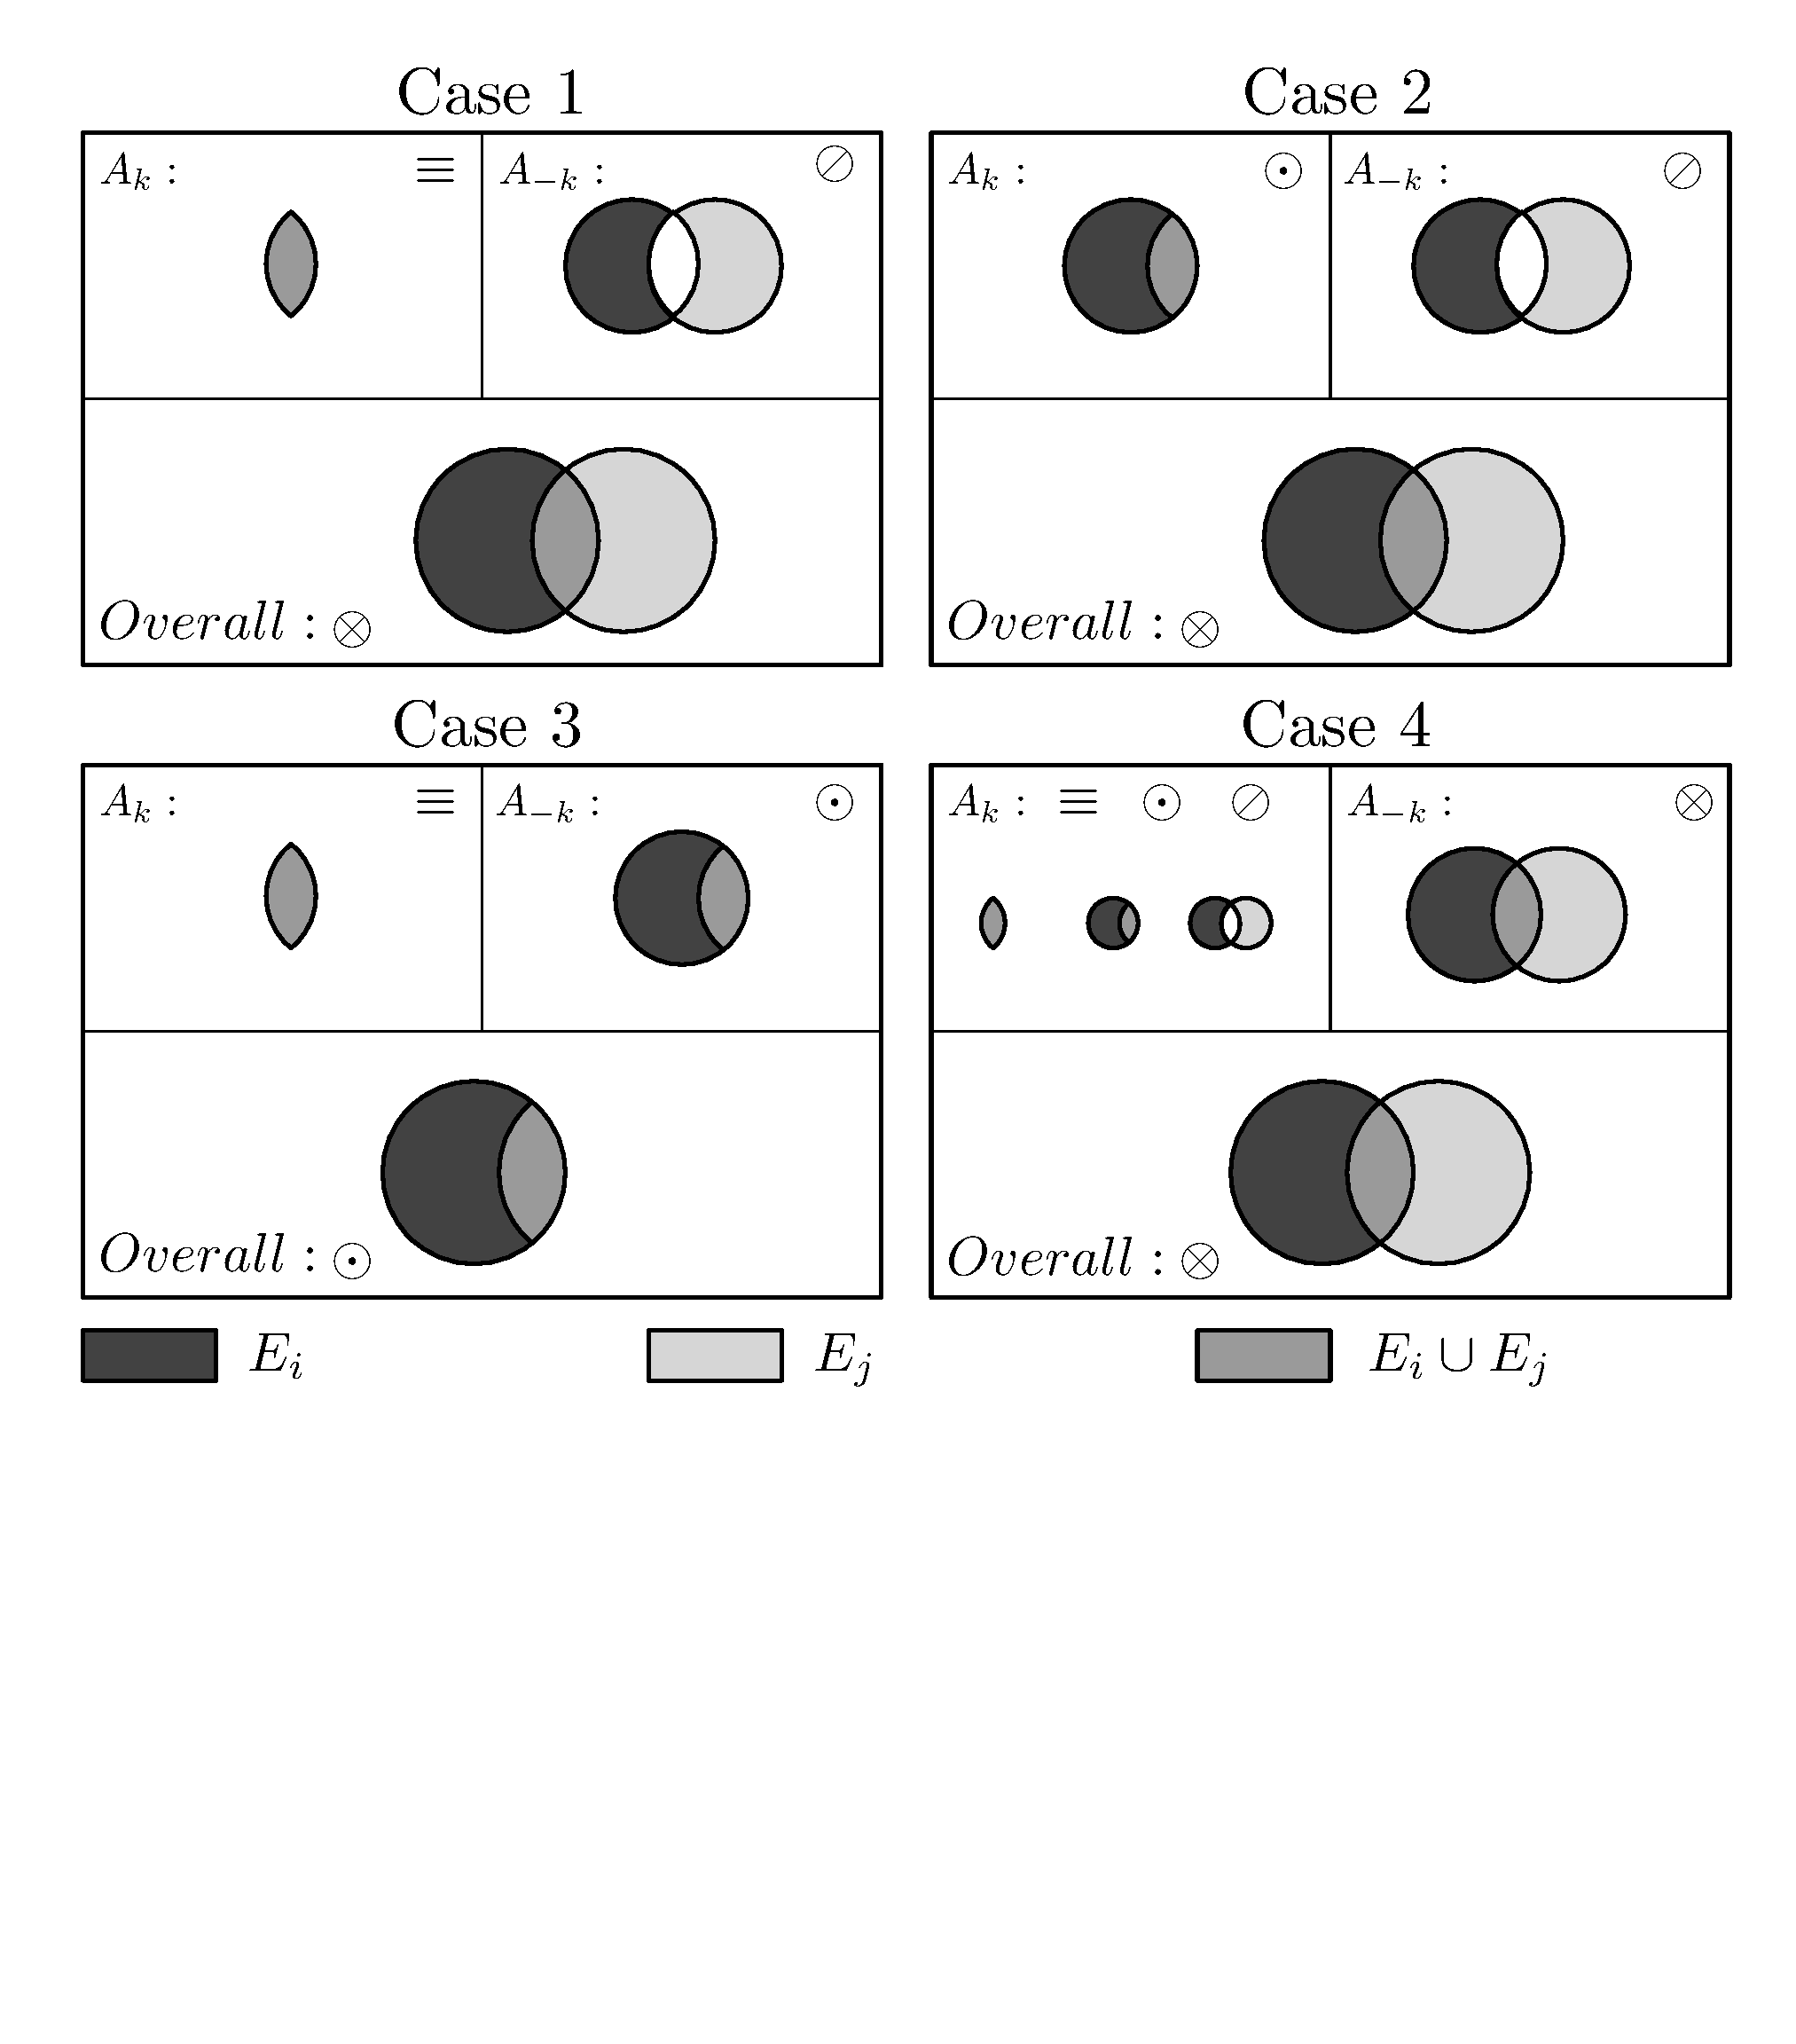
\includegraphics[scale=0.35]{figs/cases.pdf}
\caption{Venn diagrams illustrating of the four cases where it is possible to infer an overall relations' type from its two corresponding local relations' types.}
\end{figure}

\begin{restatable}[Overall Pairing Relation of Different Local Relations]{thm}{rOverall}
\label{thm:ROverall}

Let $A_{1}$ and $A_{2}$ be two agents, $A_{1}$ partitioning the context $U_{1}$ in the contrast set $K_{1} = \{ U_{1}, S_{1} \}$ and $A_{2}$ partitioning the context $U_{2}$ in the contrast set $K_{2} = \{ U_{2}, S_{2}\}$. Let $C_{i}$ and $C_{j}$ be two concepts such that $C_{i} \in S_{1}$ and $C_{j} \in S_{2}$. Let $C_{i} r_{U1} C_{j}$ be the local pairing relation of the agent $A_{1}$ and $C_{i} r_{U2} C_{j}$ the local pairing relation of the agent $A_{2}$, if $C_{i} r_{O} C_{j}$ is the overall pairing relation of $A_{1}$ and $A_{2}$ between $C_{i}$ and $C_{j}$, then the following holds:

\begin{enumerate}
\item if $C_{i} \equiv_{U1} C_{j}$ and $C_{i} \oslash_{U2} C_{j}$, then $C_{i} \otimes_{O} C_{j}$ %\textbf{(case 1)}.
\item if $C_{i} \odot_{U1} C_{j}$ and $C_{i} \oslash_{U2} C_{j}$, then $C_{i} \otimes_{O} C_{j}$ %\textbf{(case 2)}.
\item if $C_{i} \equiv_{U1} C_{j}$ and $C_{i} \odot_{U2} C_{j}$, then $C_{i} \odot_{O} C_{j}$ %\textbf{(case 3)}.
\item if $C_{i} \equiv_{U1} C_{j}$, $C_{i} \odot_{U2} C_{j}$ or $C_{i} \oslash_{U1} C_{j}$ and $C_{i} \otimes_{U2} C_{j}$, then $C_{i} \otimes_{O} C_{j}$ %\textbf{(case 4)}.
\end{enumerate}

\end{restatable}

\begin{proof}
See Appendix \ref{ap:3}
\end{proof}

At last, since the r-triplets of the pairing relations of equivalence, disjunction and overlap are symmetrical (let $R$ be a r-triplet that corresponds to a relation equivalence, disjunction or overlap. We can observe in Definition \ref{def:Relation} that in these three cases, $R = RJ$), if two local pairing relations are both equivalences, disjunctions or overlaps then the overall pairing relation will be from the same type. For the remaining cases, the agents have no choice but to exchange their local r-triplets instead of their local pairing relations in order to infer the overall pairing relation.

\section{Agreement and Disagreement}\label{sec:AgreeDisagree}

\subsection{Mutual Intelligibility and Monotonicity}\label{sec:MutInt}

The argumentation on meaning revolves around mutual intelligibility. Mutual intelligibility is context dependent, and refers to a state of the multi-agent system where both agents are able to name every example from a given context with the same sign. Since the agents are not meant to go through an extensive naming game over an entire context outside of the experimental context of our thesis, mutual intelligibility refers also to a state where both agents agree that there is no example from a given context that they would -- to their knowledge -- name differently than the other agent.

The notion of mutual intelligibility is attached to two properties. First, both agents should partition the context of their mutual intelligibility into the same segregates, at least theoretically. Then, both agents should map these segregates to the same signs. Having these two properties, equal partition and equal sign-mapping for both agents, guarantees the mutual intelligibility between the agents over a given context. This notion of mutual intelligibility is formalized in Definition \ref{def:MIntel}.

\begin{restatable}[Mutual Intelligibility]{df}{mIntel}\label{def:MIntel}
Let $A_{1}$ and $A_{2}$ be two agents that have for respective contrast sets $K_{1} = (U_{1},S_{1})$ and $K_{2} = (U_{2},S_{2})$.  $A_{1}$ and $A_{2}$ have reached mutual intelligibility under the limits of a context $U$ whenever $\forall e \in U$, $!\exists C_{i} \in S_{1}$ and  $!\exists C_{j} \in S_{2}$ such that $C_{i} \sqsubseteq e$ and $C_{j} \sqsubseteq e$ and $s(C_{i}) = s(C_{j})$. 
\end{restatable}

Now that we stated multiple times that the ultimate goal of our agents is to reach mutual intelligibility and that we have formally defined this mutual intelligibility, we need to address the question of the mutual intelligibility's context. Since the mutual intelligibility is context dependant, the agents need know over which context they are trying to reach it in order to coordinate. We will assume that this context has examples from both agents, that are however not in both current contrast sets' context, which is the most complex possible scenario. In this scenario, each agent $A_{k}$ could send to the other agent $A_{-k}$ the set of the examples from $U_{k}$ that are not in $U_{-k}$. However, this requires for each agent $A_{k}$ to know which are these examples and thus have knowledge over $U_{-k}$.

Another solution that does not necessitate for $A_{k}$ to have knowledge over $U_{-k}$ is to know the pairing relations between the concepts that have examples in the context $U$ over which the mutual intelligibility is wished. Theorem \ref{thm:RMIntel} draws a direct correspondence between the definition of a mutual intelligibility over the context $U$ and the pairing relations between concepts in $U$. 

\begin{restatable}[Constraints on Relations for Mutual Intelligibility]{thm}{RMIntel}
\label{thm:RMIntel}
Let $A_{1}$ and $A_{2}$ be two agents with contrast sets $K_{1} = (U_{1},S_{1})$ and $K_{2} = (U_{2},S_{2})$. Let $U$ be a context such that $U \subseteq U_{O}$. We say that $A_{1}$ and $A_{2}$ have reached mutual intelligibility within the context $U$ according to Definition \ref{def:MIntel} if for each concept $C_{i} \in S_{1}$ whenever either:

\begin{itemize}
    \item[a.] $\forall C_{j} \in S_{2}, C_{i} \circleddash_{U} C_{j}$ 
\end{itemize}

holds, or (\textbf{exclusive or}) all of the following holds:

\begin{itemize}
    \item[b.] $!\exists C_{k} \in S_{2}$ such that $C_{i} \equiv_{U} C_{k}$
    \item[c.] \textbf{and} $\forall C_{j} \in S_{2}$, one of the two following holds:
    \begin{itemize}
    \item[$c1$.] $C_{i} \equiv_{U} C_{j}$
    \item[$c2$.] $C_{i} \oslash_{U} C_{j}$
    \end{itemize}
    \item[d.] \textbf{and} $ \forall C_{j} \in S_{2}$:
    \begin{itemize}
        \item[$d1$.] if $C_{i} \equiv_{U} C_{j}$ then $s(C_{i}) = s(C_{j})$
        \item[$d2$.] if $C_{i} \oslash_{U} C_{j}$ then $s(C_{i}) \neq s(C_{j})$
    \end{itemize}
\end{itemize}

\end{restatable}

\begin{proof}

\end{proof}

With Theorem \ref{thm:RMIntel} the agents can now infer a mutual intelligibility over the context $U$ from the overall pairing relations of the concepts involved in the context $U$. The agents can figure the overall pairing relations between concepts by exchanging r-triplets as explained in Section \ref{sec:Overall}. Therefore, the agents do not need to exchange examples in order to know if they have reached a mutual intelligibility over a context -- even if examples of this context are not shared by both agents.

While we repeatedly asserted that the aim of the argumentation between our two agents is to reach mutual intelligibility, the mutual intelligibility itself cannot be the only goal. We can intuitively think of two unsatisfying solutions that always guarantee a mutual intelligibility; the first one is having both agents' current contrast sets $K_{1} = \{U_{1}, S_{1} \}$ and $K_{2} = \{U_{2}, S_{2} \}$ with $S_{1} = \{ C_{i} \}$ and $S_{2} = \{ C_{j} \}$ such that $C_{i}$ and $C_{j}$ both have the same sign $s_{all}$ and an intensional definition that subsumes all possible examples. In a such scenario, any example would be immediately be named $s_{all}$ by both agents which is, by definition, a mutual intelligibility. The second scenario would be one agent $A_{1}$ copying the current contrast set $K_{2} = \{U_{2}, S_{2} \}$ of the other agent $A_{2}$. In this situation, the agents have the same contrast set $(K_{1} = K_{2})$ and therefore have reached mutual intelligibility over any context that is a subset of $U_{2}$.

These in these two scenarios, mutual intelligibility has been reached over large contexts. However, if we assume that the initial contrast sets of the agents are a classification that had a purpose, we wish to have any current contrast set also able to fit this purpose no matter no matter what it is. For this reason, the agents only have current contrast sets that are \emph{refinement} of their initial contrast set. By making sure that its new contrast sets are refinements of its initial one, an agent has the guarantee that two examples initially classified in different concept remains labelled as belonging to different classes. This monotonic evolution of contrast sets is formalized in Definition \ref{def:SCon}. 

\begin{restatable}[Monotonicity]{df}{sCon}
\label{def:SCon}
Let $A$ be an agent that has an initial contrast set $K^{0} = \{U_{0}, S_{0} \}$. If $A$ creates a new contrast set $K_{1} = \{U_{1}, S_{1} \}$ as its current contrast set, $A$'s contrast sets are monotone if $U_{0} \subseteq U_{1}$, and if for all pairs of examples $e_{1},e_{2} \in U_{0}$ and for every concept $C_{1} \in S_{1}$, there exists $C_{0} \in S_{0}$:

\begin{center}
$e_{1},e_{2} \in E(C_{1}) \Rightarrow e_{1},e_{2} \in E(C_{0})$
\end{center}

\end{restatable}

\subsection{Agreement over Meaning}\label{sec:Agree}

The mutual intelligibility and the monotonicity are the formalizations of the agents goal during the argumentation. In order to reach this goal, the agents need to be able to evaluate them and identify any eventual problem that would prevent the goal's realisation.

\subsubsection{Synchronic Agreement}\label{sec:SynAg}

The synchronic agreement is a state of one agent where this agent cannot find any overall pairing relation that would contradict the mutual intelligibility as defined in Theorem \ref{thm:RMIntel}. When both agents are in a state of synchronic agreement, we say that the agents have reached mutual intelligibility.

Unlike the mutual intelligibility, the synchronic agreement can be unilateral. This occurs when one agent has access to more overall relations than the other. In this case, the former agent can know about the situation of a pair of concepts that does not satisfy the criteria listed in Definition \ref{def:MIntel} as presented in Theorem \ref{thm:RMIntel}, while the latter agent ignores the situation of this pair of concepts.

\subsubsection{Diachronic Agreement}\label{sec:DiaAg}

The diachronic agreement is a state of one agent where this agent current contrast set is a refinement of this agent initial contrast set as defined in Definition \ref{def:SCon}. Unlike the synchronic agreement, the diachronic agreement is always verified. Since the monotonicity is a constraint put on the creation of new contrast sets, no current contrast set can be created in a non-monotonic way.

\subsection{Types of Disagreements}\label{sec:Disagree} 

\subsubsection{Synchronic Disagreements}\label{sec:SynD}

The Theorem \ref{thm:RMIntel} gives, for a list of pairs of concepts and a context, the pairing relations and the relations between the signs that the two concept of each pair should observe in order to have a mutual intelligibility between the agents. If one pair of concept does not observe these properties in the context of the expected mutual intelligibility, the agents do not have the mutual intelligibility. We call such a pair a synchronic \emph{disagreement}. The notion of synchronic disagreement is defined below:

\begin{restatable}[Synchronic Disagreement]{df}{synDg}
\label{def:SynDg}
Let $A_{1}$ and $A_{2}$ be two agents that have for respective contrast sets $K_{1} = (U_{1},S_{1})$ and $K_{2} = (U_{2},S_{2})$. Let $U$ be a context such that $U \subseteq U_{1} \cup U_{2}$. Let $C_{1}$ and $C_{2}$ be two concepts such that $C_{1} \in S_{1}$ and $C_{2} \in S_{2}$. $A_{1}$ and $A_{2}$ have a synchronic disagreement over $C_{1}$ and $C_{2}$ within context $U$ whenever one of the following conditions holds:

\begin{enumerate}
\item $C_{i} \odot_{U} C_{j}$
\item $C_{i} \otimes_{U} C_{j}$
\item $C_{i} \dagger_{U} C_{j}$
\item $C_{i} \equiv_{U} C_{j}$ and $s_{i} \neq s_{j}$
\item $C_{i} \oslash_{U} C_{j}$ and $s_{i} = s_{j}$
\end{enumerate}

or if there exists a concept $C_{k} \in S_{k}$ while there is no concept $C_{-k} \in S_{-k}$ such that $C_{k} r_{U} C_{-k}$.

\end{restatable}


These six conditions give rise to 6 types of disagreement, defined as follows:

\paragraph{Hypo-hypernymy Disagreement} If $C_{i} \odot_{U} C_{j}$, then one concept is the  hyponym of the  other (and the second concept is the hypernym of the first). More specifically, if $r(C_{i},C_{j},U) = (1,1,0)$ then $C_{i}$ is the \emph{hypernym} of $C_{j}$, while if $r(C_{i},C_{j},U) = (0,1,1)$ $C_{i}$ is the \emph{hyponym} of $C_{j}$. A hypo-hypernymy disagreement is expressed as $(s_{i},s_{j},C_{i} \odot_{U} C_{j})$.

\paragraph{Overlap Disagreement} If $C_{i} \otimes_{U} C_{j}$, the two concepts are said to overlap. An overlap disagreement is expressed as $(s_{i},s_{j},C_{i} \otimes_{U} C_{j})$.

\paragraph{Synonymy Disagreement} If $C_{i} \equiv_{U} C_{j}$ and $s_{i} \neq s_{j}$, we have two concepts that are equivalent but their corresponding signs are different (therefore they are synonyms). A synonymy disagreement is expressed as $(s_{i},s_{j},C_{i} \equiv_{U} C_{j})$.

\paragraph{Homonymy Disagreement} If $C_{i} \oslash_{U} C_{j}$ and $s_{i} = s_{j}$,  we have two concepts that are disjoint  but their corresponding signs are equal (therefore they are homonyms). A homonymy disagreement is expressed as $(s_{i}, s_{j},C_{i} \oslash_{U} C_{j})$.

\paragraph{Untranslatability Disagreement} If $C_{i} \not \equiv_{U} \bullet$, we have a concept $C_{i}$ that cannot found a concept $C_{j}$ such that $C_{i} \equiv_{U} C_{j}$. The symbol ``$\not \equiv$'' does not refer to a paring relation here, but to the absence of a pairing relation of equivalence. Moreover, the symbol ``$\bullet$'' does not represent a specific concept, but any concept from $S_{2}$.

Each of the five first disagreement types can be represented as a triplet $(s_{1}, s_{2}, r_{U})$ where $s_{1}$ and $s_{2}$ are the signs of the first and second concepts, and where $r_{U}$ their relation in the context of the expected mutual intelligibility. Since one type of disagreement corresponds to exactly one type of pairing relation, $r$ qualifies the type of disagreement as it already qualifies the type of pairing relation. The untranslatability disagreement is a special case, noted $(s_{1}, \bullet, \not \equiv_{U})$.

\paragraph{Indistinguishable Disagreement} If $C_{i} \dagger_{U} C_{j}$, or if $C_{i}$ and $C_{j}$ do not have a pairing relation, the two concepts are said to be indistinguishable. While this disagreement cannot appear with regular (Boolean) r-triplets, it appears when we later assume a degree of error that requires integer r-triplets in Section \ref{sec:DoGGenIdea}.

\subsubsection{Classification of Synchronic Disagreements}\label{sec:SynDclass}

Other than according to their types, the synchronic disagreements can be regrouped by families. Synchronic disagreements are regrouped in main families that will later determine the approach that our agents will display to solve them. There are four families of synchronic disagreements: \emph{self}-disagreements, \emph{semantic} disagreement, \emph{lexical} disagreements and \emph{untranslatable} disagreements.

\paragraph{Semantic Disagreement} The semantic disagreements are hypo/hypernymy, overlap and indistinguishable disagreements involving two concepts from different agents, that require the refinement of one or two of the agents' concept(s) in order to be solved. Semantic disagreements require either a specific argumentation on meaning in order to create new concepts that are hyponyms of the older ones that cause the disagreement, or the deletion of one of the two concepts in the case of the indistinguishable type of disagreements.

\paragraph{Lexical Disagreement} The lexical disagreements are synonymy and homonymy disagreements involving two concepts from different agents, that require a sign change for one or more of the agents' concepts. Lexical disagreements are solved through the creation of new signs, without modifying any other type of semiotic elements.

\paragraph{Self-Disagreement} The self-disagreements can be any type of disagreements. However, unlike other families, the self-disagreements involve two concepts that are from the same agent. Due to the fact that the two concepts belong to the same initial contrast-set, which is a partition of the agent's context, a self-disagreement cannot be anything else than an overlap disagreement. Unlike overlaps that belong to the semantic disagreements, the self-disagreements are solved through a process named "border-alignment" instead of creating a new concept.

\paragraph{Untranslatable Disagreements} The untranslatable disagreements regroup the disagreements of the eponymous type. With the self-disagreement, this is the only family that does not involve two concepts from different agents, although it is because it only involves one concept. An untranslatable disagreement is solved by creating an equivalent concept to the one involve in the disagreement, and adding it to the contrast-set that misses it.


\subsubsection{Diachronic Disagreements}\label{sec:DiaD}

As explained in Section \ref{sec:DiaAg}, there is no diachronic disagreement. The fact that an agent $A$ has knowledge over its initial contrast set allows $A$ to create new concepts for its current contrast set that are not violating the diachronic agreement. The fact that the monotonicity is defined on the context of the initial contrast set, that does not change through the argumentation, ensures that no diachronic disagreement can appear following the addition of a new example to the current contrast set's context.

\subsection{Connected Sets of Disagreements}
\label{sec:SystemDisagreement}

Our approach is centered on the ability to simplify a communication issue between two agents, involving multiple concepts, into a list of smaller disagreements that each involves only two concepts. At an intermediary level between the interconnected graph of pairing relations and the pairs of disagreement, we have connected sets of disagreements.

\begin{restatable}[Connected Sets of Disagreements]{df}{ConnectedDisagreement}
\label{df:ConDisagreement}

Let $D = d_{1}, \ldots, d_{n}$ be a set of synchronic disagreements in a context $U$. Let $D_{1}$ be a set of disagreement such that $D_{1} \subseteq D$. $D_{1}$ is a connected set of disagreement from $D$ if:

\begin{itemize}
    \item $\forall d_{x} \in D_{1}$ such that $d_{x} = (s_{1}, s_{2},C_{1} r_{U} C_{2})$, $\exists d_{y} \in D_{1}$ such that $d_{y} = (s_{1}', s_{2}',C_{1}' r_{U} C_{2}')$ and $C_{1} = C_{1}'$, $C_{1} = C_{2}'$, $C_{2} = C_{1}'$ or $C_{2} = C_{2}'$
    \item $\forall d_{x} \in D_{1}$ such that $d_{x} = (s_{1}, s_{2},C_{1} r_{U} C_{2})$, $\nexists d_{z} \in \{D - D_{1}\}$ such that $d_{z}= (s_{1}'', s_{2}'',C_{1}'' r_{U} C_{2}'')$ and $C_{1} = C_{1}''$, $C_{1} = C_{2}''$, $C_{2} = C_{1}''$ or $C_{2} = C_{2}''$
\end{itemize}

\end{restatable}

Intuitively, connected sets of disagreements are disjoint subsets of a general set of disagreements -- usually the set of all the synchronic disagreements between two agents -- that are clustered according to the concepts that are causing the disagreements within them.

\section{Complement to the Notation}\label{sec:FormRemarks}

\subsection{On Concepts Sharing Signs}\label{sec:SharingSigns}
The protocol that we presented in the past sections has been tested in experimental scenarios of increasing complexity. All the scenarios are based on a data set that has been modified in order to create controlled instances of disagreements. Since sometimes the concepts $C_{i}^{k}$ from $A_{k}.K$ and $C_{j}^{-k}$ from $A_{-k}.K$ will be in a situation where $i = j$. In this situation, the concept $C_{i}$ from $A_{K}$ and the concept $C_{j}$ from $A_{k}.H$ can be both noted $C_{i}^{k}$ or $C_{j}^{k}$. In order to remove this ambiguity, we will note $C_{j'}^{k}$ the concept that belongs to $A_{k}.H$. This way, the apostrophe marks the belonging to a hypothesis. In the situation where $i \neq j$, the absence of ambiguity allows us to not put the apostrophe.

\subsection{On Hyponyms and Hypernyms}\label{sec:OnHypoHyper}
During the previous sections, four notions from linguistics (hyponymy, hypernymy, synonymy and homonymy) have been used  to characterize the relation between two concepts.  We add now a fifth notion, the co-hyponymy. A set of concepts $C_{h_{1}}, \ldots , C_{h_{n}}$ are co-hyponyms of a common hypernym $C_{H}$ if the co-hyponyms' extensional definitions $E_{h_{1}}, \ldots , E_{h_{n}}$ are a partition  of the hypernym's extensional definition $E_{H}$. The correct syntax to express co-hyponymy is: $C_{h_{1}}$ is co-hyponym \emph{of} $C_{H}$ \emph{with} $C_{h_{2}}, \ldots , C_{h_{n}}$.

\begin{restatable}[Co-Hyponyms]{df}{coHypo}
\label{def:CoHypo}
Let $C_{H}$ be a concept, $C_{1}, \ldots, C_{n}$ be $n$ concepts with $n > 2$, and $U$ a context such that:

\begin{enumerate}
    \item $\forall x \in \{1, \ldots, n\}, Adj(C_{x},U) \subset Adj(C_{H},U)$
    \item $\forall x,y \in \{1, \ldots, n\}, C_{x} \odot_{U} C_{y}$
    \item $Adj(C_{1},U) \cup \ldots \cup Adj(C_{n},U) = Adj(C_{H},U)$
\end{enumerate}

then $C_{1}, \ldots, C_{n}$ are co-hyponyms of $C_{H}$

\end{restatable}

\subsection{Computing Multiple R-Triplets and Pairing Relations}\label{sec:MultipleRelations}

When an agent computes multiple r-triplet or pairing relations, we simplify the notation of the set of elements computed. Given two sets of concepts $S_{1} = \{C_{1,1}, \ldots, C_{1,m} \}$ and $S_{2} = \{C_{2,1}, \ldots, C_{2,n} \}$, the set of R-Triplets $T(S_{1} \times S_{2}, U)$ is equal to:

\begin{center}
    $\{ r(C_{1,1}, C_{2,1}, U)$, $\ldots$, $r(C_{1,1}, C_{2,n}, U)$,\\
    $\ldots$\\
    $r(C_{1,m}, C_{2,1}, U)$, $\ldots$, $r(C_{1,m}, C_{2,n}, U) \}$
\end{center}


and the set of pairing relations $R(S_{1} \times S_{2}, U)$ is equal to:

\begin{center}
    $\{ C_{1,1} r_{u} C_{2,1}$, $\ldots$, $C_{1,1} r_{u} C_{2,n}$,\\
    $\ldots$\\
    $C_{1,m} r_{u} C_{2,1}$, $\ldots$, $C_{1,m} r_{u} C_{2,n} \}$
\end{center}

\subsection{R-Triplets and Associated Pairing Partial Sets}

The presentation of r-triplets in Section \ref{sec:Relations} introduced how each value of a r-triplet figures the state of emptiness of a particular pairing partial set. Let $C_{i}$ and $C_{j}$ be two concepts, $U$ a context and $U_{-1}, U_{0}$ and $U_{1}$ three partial sets such that:

\begin{itemize}
    \item $U_{-1} = U_{C_{i},\overbar{C_{j}}}$,
    \item $U_{0} = U_{C_{i},C_{j}}$ and 
    \item $U_{1} = U_{\overbar{C_{i}},C_{j}}$.
\end{itemize}

Let \emph{bool(p)} be a function that takes a proposition $p$ as a parameter and returns 1 if $p$ is true and 0 if $p$ is false. The r-triplet $r = r(C_{i}, C_{j}, U)$ is, according to \ref{def:RTriplet}, ($bool(|U_{-1}| \geq 0)$, $bool(|U_{0}| \geq 0)$, $bool(|U_{1}| \geq 0)$). We say that each element $b_{x} = bool(|U_{x}| \geq 0)$ of $r$ is the \emph{value} of $r$ of \emph{index} $x$, that is associated to $U_{x}$. Reciprocally, each pairing partial set $U_{x}$ is associated to the value $b_{x}$ of index $x$ in $r$. The value associated to a pairing partial set $U_{x}$ is noted $b(U_{x})$, and the pairing partial set associated to a value $b_{x}$ is noted $U(x)$.

\chapter{Argumentation Model}\label{ArgumentationModel}
\section{A Two Agents Model}\label{sec:AgentModel}

All the models and strategies that we explore later in the experiments show similar features. This is due to the fact that each of these models and strategies derives from a unique model that features two agents. These two agents are defined by a set of functions that they both share, by some knowledge that they only partially share and by a set of states which they can go in, each state deciding the agents' actions during the argumentation.

The different models of argumentation on the meaning varies by the error management of the model's machine learning component. On the other hand, the different strategies of argumentation on the meaning varies by the set of states in which the agents can go in.

We qualify our model as symmetrical, since for a given model and strategy the set of functions of the agents is identical, the set of states of the agents is identical, and the knowledge shared by one agent is also shared by the other.

\subsection{Agent Knowledge}

While we are in the position of an oracle and have access to the entire knowledge of both agents, each agent has itself limited knowledge over the elements that are belonging to the other agent.

In order to clarify to which knowledge which agent has access to, we are classifying the agents' knowledge in three categories: \emph{personal} knowledge, \emph{overall} knowledge and \emph{inferred} knowledge.

The personal knowledge is only accessible to one agent $A_{k}$. The overall knowledge is accessible to both agents $A_{k}$ and $A_{-k}$. The inferred knowledge is a knowledge accessible to $A_{k}$ that is mirroring, with a varying degree of accuracy, a knowledge either only accessible to $A_{-k}$ or a knowledge accessible neither to $A_{k}$ or $A_{-k}$.

\subsubsection{Personal Knowledge}

An agent $A_{k}$ has access to a contrast set, called the initial contrast set $K^{0}_{k}$, and all the elements from this contrast set -- the contrast set's concepts and the semiotic elements from these concepts. Agents can also create new contrast sets. If an agent comes to create a new contrast set, called the \emph{current} contrast set $K_{k}$ by opposition to the initial one, this agent has also access to this contrast set. When we mention a contrast set without precision on whether it is the initial or current contrast set, it is by default the current contrast set.

\subsubsection{Overall Knowledge}

The overall knowledge is the knowledge that one agent shares, at least partially, with the other agent. This category of knowledge can be divided in two categories: the \emph{shared} knowledge that is directly shared with the other agent through messages, and the \emph{inferred} knowledge that is deduced from the other agent's knowledge without being directly exchanged by messages.

\paragraph{Shared Knowledge}

The shared knowledge is transmitted through messages. Since a message can only contain either semiotic elements or triplets, the shared knowledge is limited to some semiotic elements from both agents and their relations. Since exchanging messages has a cost, the agents try to reduce the amount of shared knowledge during an argumentation. The examples that an agent has sent or received are recalled in a specific set, noted $U_{ex}$. This set of example helps the agent to not exchange an example twice, and is used to infer additional knowledge. The generalizations, always exchanged by sets corresponding to intensional definitions, can be stored in an agent $A_{k}$'s hypothesis $H_{k}$ when they are received. The intensional definitions are always received with an associated sign. While the hypothesis of an agent contains concepts and not intensional definitions alone, only the intensional definitions of the hypotheses' concepts and their signs are shared by both agents. The extensional definitions from the hypotheses' concepts are only inferred by the agent. The triplets received are used to infer overall triplets and overall pairing relations, which is discussed in the \emph{inferred knowledge} paragraph.

\paragraph{Inferred Knowledge}

From the intensional definitions received by an agent, the other agent can infer an approximation of the other agent's concept associated extensional definition (see Section \ref{sec:funCreaConI}) by using its own adjunct set instead. This allows the agent to create a new concept that can be stored in its hypothesis, which represents the agent's guess on the concepts of the other agent. An agent can infer the overall relation between one of its concept and one of the other agent's concept as described in Section \ref{sec:Overall}. Once an overall pairing relation has been inferred, this agent can identify if this pairing relation induces a disagreement. If the paring relation is causing a disagreement, this disagreement is formalized into a triplet (see Section \ref{sec:SynD}) and recalled in a set of active disagreements $D$.

The distinction between personal knowledge and inferred knowledge is perfectly illustrated in the Section \ref{sec:Knowledge} with the beliefs and arguments. While an e-argument represents a knowledge that is known as a fact by an agent, a belief represents a knowledge that the agent has inferred but is partially unsure of. Personal knowledge is exchanged by an agent to attack the inaccurate parts of the inferred knowledge of another agent. On the other hand, shared knowledge is supposed to be known by both agents and therefore should not be exchanged at all.

\subsection{Agent Modus Operandi}
\label{sec:ModusOperandi}

The argumentation takes place turn by turn, with one agent receiving a token at the beginning of the argumentation, taking a set of actions, then passing the token to the other agent. An agent can take actions only when it has the token, and the last action that it takes is always to pass the token to the other agent. The token is exchanged until termination is detected. The actions taken by an agent while it has the token are decided by the agent's inputs and its current state. The two variables that impact the behaviour of one agent at a given turn are the agent's state (a qualitative variable) and the messages that this agent has received from the other agent. Each agent has the same set of possible states, making our argumentation model \emph{symmetric}.

The argumentation model is also synchronized, meaning that if an agent $A_{1}$ is in a state \#1 during the turn $t$, the agent $A_{2}$ was either in the state \#1 during the previous turn $t_{-1}$ or will be in the state \#1 during the next turn $t_{+1}$.

\subsection{Agent Functions}

\subsubsection{Inductive Learning}

\label{sec:funIndLearn}
The agents are inductive learners. Being able to use inductive learning over a set of examples in order to obtain a set of generalizations that subsume these examples without subsuming the rest of the subset is the most fundamental function of our agents. Each agent use the ABUI algorithm in order to achieve inductive learning. An agent $A$ with a local context $U_{k}$ needs to split its context in two subsets $E$ and $E'$ such that $E \cup E' = U_{k}$ and $E \cap E' = \emptyset$. Once these two sets of examples have been created and passed as inputs of ABUI, ABUI returns an intensional definition $I = \{g_{1}, \ldots, g_{n}\}$ such that:

\begin{itemize}
\item $\forall e \in E, \exists g \in I$ such that $g \sqsubseteq e$
\item $\forall e \in E', \nexists g \in I$ such that $g \sqsubseteq e$
\end{itemize}

The ABUI algorithm cannot always guarantee that the intensional definition returned verifies these two properties, but it approaches them as much as it can by minimizing the number of examples from $E'$ that are subsumed by $I$, and the number of examples from $E$ that are not subsumed by $I$. While the rest of this section does not take into account these errors of first and second order, their impact is discussed later in Section \ref{sec:DoGGenIdea}.

\subsubsection{Naming Examples}
\label{sec:funName}

The agents can name the examples presented to them. When an agent names an example $e$, it always uses a left-path associations to find $e$'s associated sign. The container used by the agent to name $e$ is its current contrast set $K$, or the initial contrast set if no current contrast set had been created by the agent. When naming an example $e$ with its contrast set $K$, an agent returns the set of signs $\{s_{1},...,s_{n}\}$ such that $e \prescript{l}{K}{\mapsto} \{s_{1},...,s_{n}\}$.

\subsubsection{Sending and Receiving Messages}
\label{sec:funMessages}

An agent can send a message to another agent. A message has two parts: a performative and a content.
The performative of the message indicates to the other agent the intent of the message, while the content vehicles a knowledge that the sender has.
The different types of messages are presented in Appendix \ref{apx:Messages} along with their associated performatives and contents.

When an agent sends a message, it arrives in the mailbox of the other agent. The message stays in the mailbox until the other agent removes it. In Section \ref{sec:ModusOperandi}, we mentioned that agents were taking actions turn by turn. These actions are mostly determined by the state of an agent during its turn, but also by the messages that are in the mailbox. It can happen that a message from an agent $A_{1}$ is not supposed to be read by an agent $A_{2}$ before $A_{2}$ is a certain state. For this reason, each message is timed for a defined state noted \#State. The message will only be delivered to the other agent when this agent enters the timed state for the next time.

For instance, in our model, the agents $A_{1}$ and $A_{2}$ goes through two states \#1 and \#2 where they respectively evaluate the local r-triplets of each other, and the overall r-triplets of each other. Let's assume that $A_{1}$ enters State \#1 first. It is supposed to have received (local) r-triplets from \emph{Evaluation} messages sent by $A_{2}$, and to compare these r-triplets with its own local r-triplets. Doing so allows $A_{1}$ to find the overall r-triplets, as explained in \ref{sec:Overall}. After this, $A_{1}$ sends the overall r-triplets that it just found to $A_{2}$ with an \emph{Evaluation} message, and passes the token to $A_{2}$. Upon receiving the token, $A_{2}$ enters State \#1 and follows the same instructions as $A_{1}$ did during the previous turn. However, additionally to the \emph{Evaluation} messages containing the local r-triplets from $A_{1}$ that any agent is supposed to have received at the beginning of State \#1, $A_{2}$ has also received the overall r-triplets sent by $A_{1}$ during the previous turn, and that are not needed until State \#2. Since both sets of messages carry the same performative and the same type of content, $A_{2}$ does not know which r-triplet it is supposed to consider as local r-triplets to compute the overall r-triplets, and which r-triplets it is supposed to ignored. Timing the \emph{Evaluation} messages sent by $A_{1}$ during State \#1 in order for them to be received by $A_{2}$ only when $A_{2}$ enters State \#2 solves this issue.

The notation of a message is the following; a message with:

\begin{itemize}
    \item a performative \emph{Performative},
    \item a content $T = \{ T_{1}, \ldots, T_{}n \}$ were each $T_{i}$ is a different type of content, and
    \item timed for the agent state \#State
\end{itemize}

is noted \emph{Performative}\#State($T_{1}$, $\ldots$, $T_{n}$)

\subsubsection{Computing Adjunct Sets}
\label{sec:funCompAdj}

After naming examples, the most basic function that an agent should have is to compute adjunct sets of concepts. This function links the left-path and the right-path associations by retrieving the set of examples subsumed by the intensional definition of a concept. By default, the adjunct set is computed using the current contrast set of the agent. The notion of adjunct set is defined in Definition \ref{def:AdjC}. An agent $A_{k}$ computes the adjunct set of a concept $C = \langle s, I, E \rangle$ such that $I = \{g_{1}, \ldots, g_{n}\}$ by directly creating the set of examples $Adj(C,U_{k}) = \{ e \in U_{k} | \exists g \in I \wedge g \sqsubseteq e \}$.

\subsubsection{Computing Local R-Triplet and Pairing Relation}
\label{sec:funCompRT}

Using its adjunct sets, an agent $A_{k}$ can find the local pairing relation between two concepts $C_{i}$ and $C_{j}$ as explained in Section \ref{sec:Adj&Relations}. First, $A_{k}$ builds the local r-triplet $r(C_{i}, C_{j}, U_{k})$, and then computes the local pairing relation $r_{Uk}$ using Definition \ref{def:Relation}.

\subsubsection{Inferring Overall Pairing Relation from Received Triplets}
\label{sec:funInferOv}

Using the composition law presented in Theorem \ref{thm:Overall}, an agent can infer an overall pairing relation between two concepts $C_{i}$ and $C_{j}$ from a local pairing relation received from another agent and its own corresponding local pairing relation. However, the two agents need the intensional definitions of both $C_{i}$ and $C_{j}$ in order to compute their local r-triplets and infer the overall pairing relation. Once the overall relation of two concepts is obtained, the agents know if these two concepts are causing a semantic or lexical disagreement. 

In a model using Boolean r-triplets, having both local triplets is enough to find the overall relation between two concepts from different agents. However, in a model that admits a degree of error and uses integer r-triplets, the agents might need to exchange more knowledge. This problem is discussed in Section \ref{sec:DoGGenIdea}.

\subsubsection{Disagreement Listing}
\label{sec:funListD}

Finding and listing the disagreements in order to resolve them is one of the main functions of the agents. In order to resolve a disagreement, both agents should be aware of its existence and have characterized it: they should know which signs and pairing relation (or absence of relation) is behind it. That is why the disagreements are always characterized in the overall context. Before starting to resolve their disagreements, the agents should exchange enough knowledge to be certain of the nature of the eventual overall relations that cause these disagreements.

As soon as two local relations involving the two same concepts are exchanged, the agents can categorize and list the semantic, lexical or self disagreements depending on the inferred overall relation and origin of the two concepts. An untranslatable disagreement, on the other hand can only be listed to an extensive transfer of the agents' intensional definitions and the inference of all the overall pairing relations, as it is characterized by the \emph{absence} of a pairing relation.

In the case of the lazy strategy presented in Chapter \ref{LazyStrategy}, the agents do not exchange all their intensional definitions at the start of the argumentation, and therefore have to be vigilant on the fact that each concept belonging to a same system of disagreement should have an equivalent in another contrast-set.

\subsubsection{Creating New Signs}
\label{sec:funCreaSign}

Each agent can create a sign. The creation of a new sign is simple, as the signs are in an arbitrary relation with the two other semiotic elements. The created signs are ensured to be all different by keeping track of the previously created signs, and by choosing a specific structure for the new signs that differentiates them from the signs that are already existing in the agents' contrast sets. For instance, in our implementation, all the new signs start with the radical \emph{newSign\_}, followed by a unique number that is incremented each time that a sign is created.

The sign created by an agent can also be used by another agent, as long as this sign has been sent to the other agent along with the semiotic element to which it is associated.

\subsubsection{Creating New Concepts from Right-Path Associations}
\label{sec:funCreaConE}

\begin{figure}[t]
    \centering
    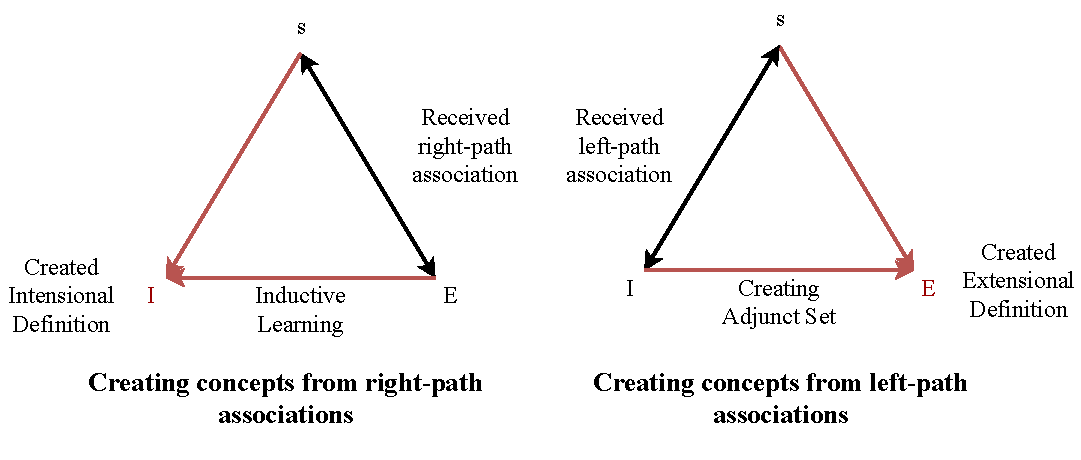
\includegraphics[width=\textwidth]{figs/ConceptCreation.pdf}
    \caption{The creation of a concept $C = \langle s,I,E \rangle$ from a right-path association (left) and a left-path association (right), by respectively retrieving the intensional definition through inductive learning and retrieving the extensional definition through the computation of the adjunct set.}
    \label{fig:ConCrea}
\end{figure}

An agent can learn a new concept if it received a set of examples associated to one sign. If the agent receives the class $U(\mapsto s)$, it can learn by inductive learning a new intensional definition $I = \{g_{1}, \ldots, g_{n}\}$ such that $I$ subsumes $U$. Other classes can be involved in the learning as negative examples: for instance, if an agent receives two classes $U_{+}(\mapsto +)$ and $U_{-}(\mapsto -)$ and wishes to create a concept that corresponds to the first class, it can learn an intensional definition $I_{+}$ that covers the examples $U_{+}$ without covering the examples $U_{-}$.

In our model, these intensional definitions are learned through inductive learning, using the ABUI algorithm. Any machine learning technique can be used to create a set of generalizations that respect these properties (only subsuming the examples from the designed class). However, in the case where an absolutely accurate learning is not guaranteed or possible, the model needs to be adapted to account a certain degree of error. The aforementioned adaptations are presented in Section \ref{sec:DoGGenIdea}.

Once the agent has created an intensional definition $I$, it creates the new concept $C = \langle s,I,U_{+} \rangle$ as the association of the three semiotic elements. Agents mostly create concepts in this fashion to create their initial contrast sets, when they receive their initial sets of right-path associations. They also use this method to generate new beliefs, when they need to cooperatively create new concepts with other agents without having an intensional definition upon which to base this creation. 

\subsubsection{Creating New Concepts from Left-Path Associations}
\label{sec:funCreaConI}

When an agent does not directly have access to the right-path associations, it can still create a concept from an intensional definition $I$ and a sign $s$ by creating the adjunct set of the concept from which $I$ and $s$ originates, as the adjunct set only requires an intensional definition to be computed. By doing so, the agent obtains a set of left-path associations. If an agent $A_{k}$ receives an association $I = \{g_{1}, \ldots, g_{n}\} \mapsto s$, it can directly create the concept $C = \langle s, I,  Adj(I,U_{k}) \rangle$.

\subsubsection{Creating New Concepts through Argumentation}
\label{sec:funCreaConA}

\begin{figure}[t]
    \centering
    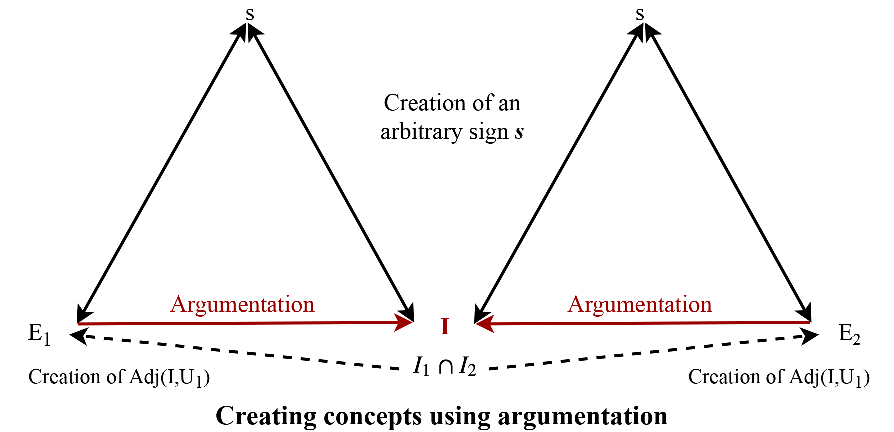
\includegraphics[width=0.78\textwidth]{figs/CoopConceptCreation.pdf}
    \caption{The creation of a new concept through the use of argumentation. The main steps are: determining an overall pairing partial sets from two intensional definitions, creating the corresponding local partial sets, arguing on the adequacy of proposed intensional definitions for the overall pairing partial set, and creating an arbitrary sign.}
    \label{fig:CoopConCrea}
\end{figure}

Creating a new concept $C_{n} = \langle s_{n}, I_{n}, E_{n} \rangle$ using either left or right-path associations requires for the agent to have at least two of $C_{n}$'s semiotic elements -- its sign and either its extensional or intensional definition. However, our model requires the agents to create new concepts which they have no semiotic element of, in order to resolve several types of disagreements. In situations like these, the agents can only create a new concept by arguing with each others.
% Define the extensional definition in the overall context

First, the two agents need to determine which subset of the overall context will be the extensional definition of a new concept. This set is noted $U_{n}^{+} = Adj(C_{n},U_{O})$, as the extensional definition of our new concept $C_{n}$ should ideally be $C_{n}$'s adjunct set according to Definition \ref{def:AdjC}.
% Cannot access the overall context, so need to decide using intensional definitions
In the context of a disagreement which involves two concepts $C_{1}$ and $C_{2}$, $U^{+}_{n}$ is determined to be one of the overall pairing partial sets $U_{O,1,\overbar{2}}, U_{O,1,2}, U_{O,\overbar{1},2}$ of $C_{1}$ and $C_{2}$. The choice of a particular set depends on the type disagreement that the agents are resolving, which we discuss later in Section \ref{sec:Resolution}.

% Positive and negative sets of examples are consistent
The relative complement of $U^{+}_{n}$ with respect to $U_{O}$ is noted $U^{-}_{n}$. Together, $U^{+}_{n}$ and $U^{-}_{n}$ partition the overall context $U_{O}$. Even if it has determined which overall pairing partial set of the pair of concept $C_{1},C_{2}$ is $U^{+}_{n}$, $A_{k}$ cannot directly access the sets $U^{+}_{n}$ and $U^{-}_{n}$ as it might contains examples from $U_{-k}$. $A_{k}$ can only access its local examples of $U^{+}_{n}$, the set $U^{+}_{n,k} = U^{+}_{n} \cap U_{k}$.

% Create a sign
The next step for the agents is to create an arbitrary sign $s_{n}$ that each agent $A_{k}$ will associate with its set of examples $U^{+}_{n,k}$. Since $s_{n}$ only has the requirement of not belonging to the agents' joint vocabulary, any agent can create $s_{n}$ and send it to the other agent. Once both agents have associated their sets of examples $U^{+}_{n,k}$ with the sign $s_{n}$, they each have a set of association $U^{+}_{n,k} \prescript{r}{k}{\mapsto} s_{n}$. One agent $A_{1}$ is then chosen to create a new intensional definition from this set of right-path associations, using the same method as for the creation of new concepts using right-path associations detailed in Section \ref{sec:funCreaConE}. $A_{1}$ is chosen accordingly to the type of disagreement that $C_{n}$ is supposed to help resolving, which we discuss later in Section \ref{sec:Resolution}.

% Change the intensional definition
Since $U^{+}_{n,1}$ is only a subset of $U^{+}_{n}$, there is an important risk that the intensional definition $I^{t1}_{1}$ which is
learned over $U^{+}_{n,1}$ subsumes examples subsumes examples that belong to the set $U^{-}_{n,2} = U^{-}_{n} \cap U_{2}$, or on the contrary does \emph{not} subsume examples from $U^{+}_{n,2}$. Since $U^{+}_{n,2}$ and $U^{-}_{n,2}$ are also subsets of respectively $U^{+}_{n}$ and $U^{-}_{n}$, a such scenario would imply that $I^{t}_{n}$ is not fit to be the extensional definition of $U^{+}_{n}$. In order to help $A_{1}$ to create a suitable intensional definition for $U^{+}_{n}$, the agent $A_{2}$ can argue about the fitness of $I^{t1}_{n}$ over $U^{+}_{n}$ so $A_{1}$ can create a more fitting intensional definition $I^{t2}_{n}$. This argumentation can be done over any intensional definition $I^{tx}_{n}$ until a final intensional definition $I^{tF}_{n}$ that is suitable for $U^{+}_{n}$ is found. The argumentation framework used to find $I^{tF}_{n}$ is discussed in Section \ref{sec:funLeadArg}.
% Creating the concept(s)
Once the intensional definition is found, each agent $A_{k}$ creates its own version of the new concept $C^{k}_{n} = \langle s_{n}, I^{tF}_{n}, U^{+}_{n,k} \rangle$. Then, $A_{1}$ adds $C^{1}_{n}$ to its contrast set while $A_{2}$ adds $C^{2}_{n}$ to its hypothesis.

\subsubsection{Managing the Creation of a New Intensional Definition}
\label{sec:funLeadArg}

As mentioned in the previous section, only one agent is in charge of a new concept's creation through argumentation while the other agent is helping by arguing over the correctness of the relation between the new concept's extensional and intensional definitions. When an agent learns that it will have to create a new concept through argumentation, it decides whether or not to take the lead according to the following rules. The agent decides to take the lead if:

\begin{enumerate}
    \item it is the only one to have examples from the positive set of examples in its context \textbf{or}
    \item it has not received a message from the other agent indicating that the other agent took the lead \textbf{and}
    \item it has examples from the positive set of examples \textbf{and}
    \item it has the right container, decided upon the type of disagreement leading to the creation of a new concept.
\end{enumerate}

When an agent takes the leadership in the creation of the new intensional definition, it immediately sends a message to the other agent indicating so.

\section{Argumentation in Concept Creation}
\label{sec:Knowledge}

\subsection{Arguments as Binary Classifications}

% Explain why we need an argumentation
Before arguing in the process of a new concept $C_{n}$'s creation, the agents have already determined the extensional definition and the sign of the new concept. The agents are however missing the intensional definition $I(C_{n})$k, and the argumentation is what will help them to find it. As we mentioned in Section \ref{sec:funCreaConA}, the main issue with finding $I(C_{n})$ is that the agents need to ensure that $I(C_{n})$ is subsuming every elements of $U^{+}_{n}$ without subsuming any element of $U^{-}_{n}$. This requires to test all the elements of the overall context, which cannot be done by one agent individually as none of the agents is supposed to have access to the overall context.

% Explain the binary classification
The agents can however overcome this issue by cooperating in the creation of $I(C_{n})$. In order to explain how, let's consider the creation of $I(C_{n})$ as a binary classification over $U_{O}$. The agents want $I(C_{n})$ to subsume the examples of the extensional definition $U^{+}_{n}$ without subsuming the other examples from $U_{O}$, $U^{+}_{n}$ is similar to a set of positive elements. Likewise, the set of examples $U^{-}_{n}$ is similar to a set of negative elements since it is the relative complement of $U^{+}_{n}$ with regard to the entire population of our test $U_{O}$. By subsuming or not the examples of $U_{O}$, $I(C_{n})$ creates another partition of $U_{O}$ into positive and negative assignments. The positive assignments of $I(C_{n})$ are the examples $\{e \in U_{O} | I(C_{n}) \sqsubseteq e \}$, which according to Definition \ref{def:AdjI} is the adjunct set of $I(C_{n})$. The set of negative assignments of $I(C_{n})$ is $\{e \in U_{O} | I(C_{n}) \not \sqsubseteq e \}$, equivalent $U_{O} - Adj(I(C_{n}),U_{O})$. In order to be an intensional definition for $C_{n}$.

% Can measure the adequateness of any intensional definition
According to Definition \ref{def:Con}, $I(C_{n})$'s set of positive assignments should be equivalent to the set of positive elements in order for $I(C_{n})$ to be an adequate intensional definition for $C_{n}$. Representing $I(C_{n})$ as a binary classification allows us to measure the adequacy of any intensional definition $I$ to the role of intensional definition of $C_{n}$ in terms of true positives, true negatives, false positives and false negatives. These four sets are defined as:

\begin{itemize}
    \item The set of true positives of $I$ is $TP(I) = \{ e \in U^{+}_{n} | I \sqsubseteq e \}$
    \item The set of true negatives of $I$ is $TN(I) = \{ e \in U^{-}_{n} | I \not \sqsubseteq e \}$
    \item The set of false positives of $I$ is $FP(I) = \{ e \in U^{-}_{n} | I \sqsubseteq e \}$
    \item The set of false negatives of $I$ is $FN(I) = \{ e \in U^{+}_{n} | I \not \sqsubseteq e \}$
\end{itemize}

% Why we need an argumentation framework
If the intensional definition has $I$ no false positives or false negatives, therefore the set of $I$'s positive assignments is equivalent to the set of positive elements and $I$ is suitable to be the intensional definition $I(C_{n})$ of the new concept $C_{n}$. Therefore, in order to be sure that $I = I(C_{n})$, the agents should agree that:

\begin{itemize}
    \item The set $FP(I) = \emptyset$
    \item The set $FN(I) = \emptyset$
\end{itemize}

As we mentioned, no agent has individually entirely access to $U^{+}_{n}$ or $U^{-}_{n}$. However, we know that the overall context is the union of the two local contexts, which means that:

\begin{itemize}
    \item $U^{+}_{n} = U^{+}_{n,1} \cup U^{+}_{n,2}$
    \item $U^{+}_{n} = U^{-}_{n,1} \cup U^{-}_{n,2}$
\end{itemize}

Therefore, the agents know that:

\begin{itemize}
    \item $U^{+}_{n,1} \cap U^{+}_{n,2} = \emptyset \Leftrightarrow U^{+}_{n} = \emptyset$
    \item $U^{-}_{n,1} \cap U^{-}_{n,2} = \emptyset \Leftrightarrow U^{-}_{n} = \emptyset$
\end{itemize}

While the agents cannot directly access $U^{+}_{n}$ and $U^{-}_{n}$, they can both locally verify that they have no knowledge of false positives or negatives and share this information in order to know if an intensional definition is suitable to be the intensional definition of $C_{n}$. Exchanging false positives and negatives is akin to an argumentation process.

% Basis of argumentation frameworks
An argumentation framework consists of a combination of a set of elements $A$ called \emph{arguments}, and a binary relation on $A$ called \emph{attack} relation. An argument $\gamma$ attacking another argument $\alpha$ is noted $\gamma \twoheadrightarrow \alpha$. An argument $\alpha$ represents a binary classification of the overall context $U_{0}$, partitioning $U_{O}$ into positive and negative assignments. Moreover, $\alpha$ should clarify which classification it intends to predict. The notion of argument is formally defined below in Definition \ref{def:Arg}:

\begin{restatable}[Argument]{df}{Argument}
\label{def:Arg}

Let $A_{1}$ and $A_{2}$ be two agents with an overall context $U_{O}$. The context $U_{O}$ is partitioned in two sets of examples $U^{a}$ and $U^{b}$. Let $a$ and $b$ be two signs such that $U^{a} \prescript{}{k}{\mapsto} a$ and $U^{b} \prescript{}{k}{\mapsto} b$ for all agents $A_{k}$. An argument $\alpha$ is a pair $(a,A_{k})$ that has an adjunct set $Adj(\alpha,U_{k}) = U^{a} \cap U_{k}$. Conceptually, the adjunct set of $\alpha$ is a binary classification function such that:

\begin{itemize}
    \item $U^{a}$ is the set of positive elements of $\alpha$
    \item $U^{b}$ is the set of negative elements of $\alpha$
    \item $Adj(\alpha,U_{O})$ is the set of positive assignments of $\alpha$
    \item $U_{O} - Adj(\alpha,U_{O})$ is the set of negative assignments of $\alpha$
\end{itemize}

and represents the fact that:

\begin{itemize}
    \item $A_{k}$ \textbf{knows} that $Adj(\alpha,U_{k}) = U^{a} \cap U_{k}$
    \item $A_{k}$ \textbf{expects} that $Adj(\alpha,U_{O}) = U^{a}$
\end{itemize}

\end{restatable}

During the process of creating a new concept, the aim of the argumentation between our agents is to generate an argument which extension is the set of examples $U^{+}_{n}$. A such argument proves that the agent that created it has enough knowledge over the overall context to generate an intensional definition suitable for the new concept.

\subsection{Evaluating Arguments}

In our argumentation framework, arguments are sorted into \emph{accepted} and \emph{rejected} arguments according to the following marking function:

\begin{itemize}
    \item an argument $\alpha$ is \emph{accepted} if none of the arguments attacking $\alpha$ is accepted, and
    \item an argument $\alpha$ \emph{rejected} if at least one of the arguments attacking $\alpha$ is accepted
\end{itemize}

Our argumentation framework is generative, meaning that instead of having a set of arguments and attacks before hand over which we apply a label function that determines which of these arguments are accepted, an agent $A_{k}$ can decide whether or not an argument $\alpha$ from the other agent should be acceptable in the first place. If $\alpha$ should not be acceptable and yet is accepted, $A_{k}$ can generate another argument $\gamma$ such that $\gamma \twoheadrightarrow \alpha$. The argument $\alpha$ being attacked makes it automatically defeated.

In order to determine whether or not an argument $\alpha$ is acceptable, an agent $A_{k}$ searches for false positives and negatives. According to Definition \ref{def:Arg}, we can write the false positives and false negatives of the argument $\alpha$ as follow:

\begin{itemize}
    \item \textbf{FP($\alpha$)} = $U^{b} \cap Adj(\alpha,U_{O})$
    \item \textbf{FN($\alpha$)} = $U^{a} \cap (U_{O} - Adj(\alpha,U_{O}))$
\end{itemize}

From the expression of false positives and negatives of $\alpha$, we can infer a group of properties that are useful to determine how the argument $\alpha$ should be considered as acceptable by $A_{k}$.

\begin{restatable}{pp}{FPalpha}
\label{pp:FPalpha}
Let $A_{1}$ and $A_{2}$ be two agents with an overall context $U_{O}$. Let $U_{O}$ be partitioned in two sets of examples $U^{a}$ and $U^{b}$, and let $\alpha = (a,A_{-k})$ be an argument of $A_{-k}$. The set of $\alpha$'s false positives in $U_{k}$ is empty if and only if FP($\alpha$) is empty.

\end{restatable}

\begin{restatable}{pp}{FNalpha}
\label{pp:FNalpha}
Let $A_{1}$ and $A_{2}$ be two agents that have their overall context $U_{O}$ partitioned in two sets of examples $U^{a}$ and $U^{b}$, and let $\alpha = (a,A_{-k})$ be an argument of $A_{-k}$. The set of $\alpha$'s false negatives in $U_{k}$ is empty if and only if FN($\alpha$) is empty.

\end{restatable}

\begin{restatable}{pp}{Adequacy}
\label{pp:FNFPaccept}

Let $A_{1}$ and $A_{2}$ be two agents that have their overall context $U_{O}$ partitioned in two sets of examples $U^{a}$ and $U^{b}$, and let $\alpha = (a,A_{-k})$ be an argument of $A_{-k}$. If the set of $\alpha$'s false positives and $\alpha$'s false negatives in $U_{k}$ are both empty, then $Adj(\alpha,U_{O}) = U^{a}$.

\end{restatable}

\subsubsection{Counter-Argument}

% If both FP(alpha) and FN(alpha) are empty, then expectations of A_{-k} were right and alpha should be accepted
Property \ref{pp:FNFPaccept} states that if both FP($\alpha$) and FN($\alpha$) are empty, then the expectations of $A_{-k}$ were right as $Adj(\alpha,U_{O}) = U^{a}$. This means that if $A_{k}$ does not find false positives or negatives of $\alpha$ in its local context, then $A_{k}$ should accept the argument $\alpha$.
% Otherwise, send an argument to A_{-k} to inform that there are true/false positives.
Otherwise, $A_{k}$ should generate another argument $\gamma$ for each set of $FP(\alpha), FN(\alpha)$ which is non empty, such that $\gamma \twoheadrightarrow \alpha$. We say that $\gamma$ is a counter-argument. The notion of counter argument is defined below in Definition \ref{def:CArg} :

\begin{restatable}[Counter-Argument]{df}{CArgument}
\label{def:CArg}

Let $A_{1}$ and $A_{2}$ be two agents that have their overall context $U_{O}$ partitioned in two sets of examples $U^{a}$ and $U^{b}$, and let $\alpha = (a,A_{-k})$ be an argument of $A_{-k}$. The argument $\gamma = (x,A_{k})$ of $A_{k}$ is a counter argument  such that $\gamma \twoheadrightarrow \alpha$ if:

\begin{itemize}
    \item $Adj(\gamma,U_{k}) = FN(\alpha)$, if $x = a$
    \item $Adj(\gamma,U_{k}) = FP(\alpha)$, if $x = b$
\end{itemize}

\end{restatable}

The definition of counter arguments makes them arguments, implying that counter arguments can be attacked by other counter arguments, building up a tree that we call the argumentation tree.

\subsubsection{Accepted vs. Agreed Upon}

Each argument in the argumentation tree is either accepted or rejected. The function that marks the arguments as accepted and rejected is called the marking function. Each time that a new argument appears in the argumentation tree, the marking of the arguments change. There is a difference between an argument $\alpha = (a,A_{k})$ that is accepted because $A_{-k}$ did not have the opportunity to generate an attack against $\alpha$ yet, and an argument $\alpha'$ that has been considered acceptable by $A_{-k}$. In the former case, the marking of $\alpha$ as accepted can be temporary, while an argument $\alpha' = (a,A_{k})$ that has been deemed acceptable by $A_{-k}$ will remained accepted. This difference is marked by the conceptual distinction between \emph{accepted} arguments, that are just temporary marked as accepted, and arguments \emph{agreed upon}, that are definitively marked as accepted.

\subsection{Root Arguments}

\begin{figure}[t]
    \centering
    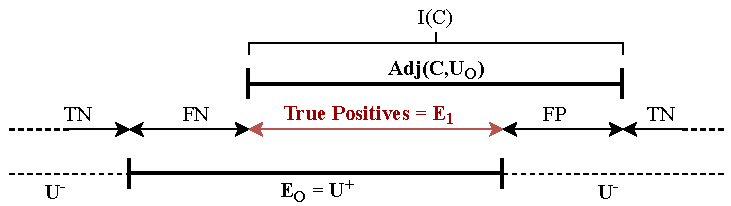
\includegraphics[width=\textwidth]{figs/Belief.pdf}
    \caption{The examples subsumed by an intensional definition $I(C)$ (top bracket) might be different from the examples that $I(C)$ is intended to subsume, especially if $I(C)$ was created without access to some of these examples. These differences are either false positives for the examples subsumed by $I(C)$ that were not intended to be, and false negative for the examples that are not subsumed by $I(C)$ but were intended to.}
    \label{fig:Belief}
\end{figure}

In order to find if an intensional definition $I$ is suitable to be the intensional definition of the new concept, $I$ will be transformed into an argument and the agents will be attacking it. In order to transform any intensional $I$ definition into an argument $\alpha$, $I$ needs to be associated to a sign $s \in \{+,-\}$. The sign $s$ determines which set from $U^{+}_{n}$ and $U^{-}_{n}$ should be the set of positive elements in the binary classification. If $I$ is a candidate for the intensional definition of $C_{n}$, then $s = +$. If this is the case, $I$ is said to be a \emph{root} argument. An argument is always associated to an agents $A_{k}$ that creates it. In the case of a root argument, this agent is the agent that leads the creation of the new concept. Root arguments are defined below in Definition \ref{def:RArg}:

\begin{restatable}[Root Argument]{df}{RArgument}
\label{def:RArg}

Let $A_{1}$ and $A_{2}$ be two agents, let $I = \{ g_{1}, ..., g_{m} \}$ be a set of generalizations and  $U_{O}$ the overall context of the agents, divided in two sets of examples $U^{+}$ and $U^{-}$ that partition the overall context. A root argument $\alpha = (+,I,A_{k})$ means that:

\begin{itemize}
    \item $A_{k}$ \textbf{knows} that $I \sqsubseteq U^{+}_{n,k}$ and $\nexists e \in U^{-}_{n,k}$ such that $I \sqsubseteq e$.
    \item $A_{k}$ \textbf{expects} that $I \sqsubseteq U^{+}_{n}$ while $\nexists e \in U^{-}_{n}$ such that $I \sqsubseteq e$.
\end{itemize}

\end{restatable}

\subsubsection{Generating Root Arguments}

The set of generalization $I$ of a root argument should subsume the examples of $U^{+}_{k}$ without subsuming the examples from $U^{-}_{k}$. The task of creating $I$ is given to the ABUI algorithm. The ABUI algorithm takes two classes, $U(\mapsto a)$ and $U(\mapsto b)$, and a sign $s \in \{a, b\}$. The ABUI algorithm returns a set of generalizations $I$ that subsumes all the examples from the class $U(\mapsto s)$ without subsuming any example from the other class $U(\mapsto S-s)$. In order to obtain $I$, the ABUI algorithm is given the two classes $U^{+}_{n,k}$ and $U^{-}_{n,k}$, with the sign $+$.

The ABUI can take an additional parameter, a set of generalization-sign associations $AA = G \mapsto S$, where $G$ is a set of generalizations $\{g_{1}, \ldots, g_{j} \}$ and $S$ is the lexicon $\{ a, b \}$. While looking for a suitable set of generalizations $I = g'_{1}, \ldots, g'_{p} $ that subsumes the examples of $U(\mapsto a)$ without subsuming the examples of $U(\mapsto b)$, ABUI ensures that:

\begin{itemize}
    \item for each generalization-sign association $g \mapsto a \in AA$, there exists another generalization $g' \in I$ such that $g' \sqsubseteq g$.
    \item for each generalization-sign association $g \mapsto b \in AA$, there are no generalization $g' \in I$ such that  $g' \sqsubseteq g$.
\end{itemize}

By adding generalizations that subsumes the false positives or negatives of different arguments in $AA$, the agents decrease the chances of having ABUI outputting a generalization that subsumes false positives, while increasing the chances of outputting a generalization that subsumes false negatives. The ABUI algorithm might not find a satisfying set of generalizations for a root argument each time. An unsuccessful root argument creation translates into an empty intensional definition for the new concept and the argumentation stops immediately.

\subsubsection{Agreed Upon Root Arguments}

If a root argument $\alpha = (+,I,A_{k})$ is agreed upon, then $I$ is considered as accepted as the intensional definition of the new concept $C_{n}$. The agents have determined the three semiotic elements of $C_{n}$, and the creation of $C_{n}$ can be achieved. The argumentation in the context of the creation of $C_{n}$ can therefore stop. This is one of the two stopping condition of the argumentation on the creation of $C_{n}$, along with the generation of a root-argument with an empty intensional definition. 
 
\subsubsection{Rejected Root Arguments}

If a root argument $\alpha = (+,I,A_{k})$ created by $A_{k}$ is rejected, $A_{k}$ has two options. The argument $\alpha$ being rejected means that there are one or several counter-arguments $CA = \{\gamma_{1}, \ldots, \gamma_{m}\}$ attacking $\alpha$ that are accepted. The first option of $A_{k}$ is to generate $m$ counter-arguments that will attack all the arguments from $CA$, since $\alpha$ is rejected only if there is at least an argument from $CA$ that is not rejected.

Of course, this option is only available to $A_{k}$ if the arguments from $CA$ are not acceptable. If at least one of the arguments from $CA$ is acceptable and has been agreed upon, then $A_{k}$ needs to create another root argument in order to continue the argumentation. The improvement of the new proposed intensional definition over the intensional definition that has been rejected as a root argument, is the result of the set of generalization-sign $AA$ that increases in size during the argumentation.

\subsection{G-Arguments}
\label{sec:GArg}

\begin{figure}
    \centering
    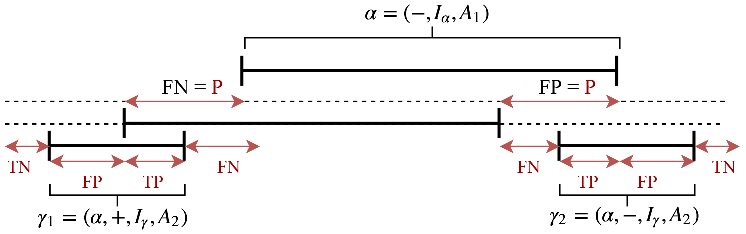
\includegraphics[width=\textwidth]{figs/Attack.pdf}
    \caption{As a belief, the intensional definition of a g-argument $\gamma$ intents to subsume the examples of a defined set (the false positives in the case of $\gamma_{1}$ or the false negatives in $\gamma_{2}$, of the belief $_{\alpha}$ that it attacks). Therefore, it also admits its own sets of false positives and false negatives, that can be attacked by other arguments themselves.}
    \label{fig:Attack}
\end{figure}

The root arguments are not the only class of arguments. The most similar class of argument to the root argument is the g-argument. Akin to the root arguments, the g-arguments are using an intensional definition to define their adjunct sets. However, since the g-arguments are not root arguments, they are always attacking another arguments and therefore are always counter arguments. The notion of g-argument is defined below in Definition \ref{def:GArg}:

\begin{restatable}[G-Argument]{df}{GArgument}
\label{def:GArg}

Let $A_{1}$ and $A_{2}$ be two agents that have their overall context $U_{O}$ partitioned in two sets of examples $U^{a}$ and $U^{b}$, and let $\alpha = (a,A_{-k})$ be an argument of $A_{-k}$. The g-argument $\gamma = (x,I,A_{k})$ is a counter argument of $A_{k}$ such that: 

\begin{itemize}
    \item for any context $U$, $Adj(\gamma,U) = Adj(I,U)$ and
    \item $Adj(I,U_{k}) = FN(\alpha)$, if $x = a$ or
    \item $Adj(I,U_{k}) = FP(\alpha)$, if $x = b$ or
\end{itemize}

\end{restatable}

\subsubsection{Accepted G-Arguments}

Every time that a g-argument gets accepted, the sets of accepted and rejected arguments of the argumentation tree are updated. If a g-argument $\gamma = (x,I,A_{k})$ stays accepted after the agent $A_{-k}$ had the opportunity to add a counter argument to the argumentation tree, the association $\gamma \mapsto x$ is added to the parameter $AA$ of the ABUI algorithm for the rest of the argumentation over the creation of $C_{n}$. 

\subsubsection{Rejected G-Arguments}

A rejected g-argument $\gamma$ stays in the argumentation tree. Every time that a g-argument gets rejected, the sets of accepted and rejected arguments of the argumentation tree are updated, as the argument $\alpha$ that $\gamma$ was attacking might now be accepted.

\subsection{E-Arguments}

The last class of arguments is the e-argument. An e-argument, unlike root arguments and g-arguments, does not use an intensional definition to define their adjunct sets, but rather uses directly a set of examples $E$. Since this set of example might not be a subset of the context of the agent that did not create the e-argument, the set of example $E$ is always set through an \emph{Examples} message along with the e-argument itself. Like to the g-arguments, e-arguments are counter arguments. The notion of e-argument is defined below in Definition \ref{def:EArg}:

\begin{restatable}[E-Argument]{df}{EArgument}
\label{def:EArg}

Let $A_{1}$ and $A_{2}$ be two agents that have their overall context $U_{O}$ partitioned in two sets of examples $U^{a}$ and $U^{b}$, and let $\alpha = (a,A_{-k})$ be an argument of $A_{-k}$. The g-argument $\gamma = (x,E,A_{k})$ is a counter argument of $A_{k}$ such that: 

\begin{itemize}
    \item for any context $U$, $Adj(\gamma,U) = E$ and
    \item $E = FN(\alpha)$, if $x = a$ or
    \item $E = FP(\alpha)$, if $x = b$ or
\end{itemize}

\end{restatable}

Since e-arguments require to exchange examples with other agents, they are not the privileged option during the generation of a counter argument and an agent that rejects an argument will always prefer to create an attack with a g-argument, in order to limit the example transfers between the agents.

\subsubsection{Accepted E-Arguments}

When an e-argument $\gamma = (x,E,A_{k})$ is accepted, its set of examples $E$ is added to the context of the agent $A_{-k}$. Since the acceptability of a g-argument and a root argument are always linked to the adjunct set and therefore to the context of an agent, changing the context of $A_{-k}$ always impact which arguments are deemed acceptable by $A_{-k}$. Moreover, every time that an e-argument gets accepted, the sets of accepted and rejected arguments of the argumentation tree are updated.

\subsubsection{Rejected E-Arguments}

An e-argument $\gamma = (x,E,A_{k})$ attacking an argument $\alpha = (a,A_{-k})$ cannot be attacked. Indeed, its adjunct set is its set of positive elements. Its adjunct set being its positive assignment, the set of positive assignments of $\gamma$ is therefore its set of positive elements and there cannot be false positives or negatives of $\gamma$. For this reason, e-arguments are always leaves on the argumentation tree.

\subsection{Argumentation Tree}

\begin{figure}
    \centering
    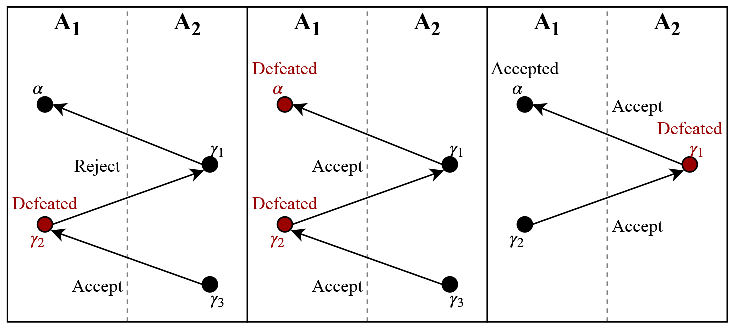
\includegraphics[width=\textwidth]{figs/Resolution.pdf}
    \caption{Once received, an argument is evaluated. If the argument is accepted, the three presented outcomes are possible. The leftmost figure represents the agent $A_{1}$ accepting the argument $\gamma_{3}$ of $A_{2}$: upon the removal of the defeated $\gamma_{2}$, $\gamma_{1}$ is re-evaluated but still rejected and therefore $A_{1}$ will build a new argument against it. The middle figure represents the agent $A_{1}$ accepting $\gamma_{3}$, and upon re-evaluating $\gamma_{1}$ accepts it as well, therefore removing the belief $\alpha$ and left with no other choice than creating a new belief. The rightmost figure represent the agent $A_{2}$ accepting the argument $\gamma_{2}$, removing the defeated argument $\gamma_{1}$ and therefore re-evaluating and then accepting the belief $\alpha$, ending the argumentation.}
    \label{fig:Resolution}
\end{figure}

The argumentation in concept creation takes place in the context of the global argumentation on meanings between the two agents, and therefore follow the same rules. The argumentation is turn by turn based, with each agent taking actions between the moment it receives the token and passes it to the other agent. The argumentation in concept creations involves arguments, and in our model these arguments are messages with specific performatives. The two performatives that are specific to the argumentation in concept creation are:

\begin{itemize}
    \item \textbf{Root-Argument, G-Argument, E-Argument}: the message is simply an argument. The type of argument decides which type of elements are contained in the message.
    \item \textbf{Accept-Argument}: the message does not have any content other than the identifier of the accepted argument.
\end{itemize}

\section{General Structure of Argumentation} 
\label{sec:ArgStruct}

\subsection{Argumentation Goal}
\label{sec:ArgumentationGoal}

When two agents meet, they are prepared to face a situation where they do not understand each other. In order to be ready for argumentation, they both create a copy of their initial contrast set. This copy of their initial contrast set becomes their \emph{current} contrast set. These current contrast sets might be modified later if the agents start an argumentation. The goal of an argumentation is always to make two agents reach mutual intelligibility without changing their contrast sets in a non-monotonic way. While the agents can chose different strategies to reach the mutual intelligibility with this constraint, all strategies have the same final goal and also share similar intermediary goals. 

While Section \ref{sec:AgreeDisagree} presents the characteristic of mutual intelligibility, this section will focus on its achievement from a point where our system of two agents is unable to guarantee it. In this section, we  stated that while the synchronic agreement was probably not initially reached by the agents, the diachronic agreement is initially always found. The diachronic agreement being always initially found is due to the fact that this agreement symbolize the similarity between the initial and the current contrast set. Since the current contrast set is initially a copy of the initial contrast set, there is initially no difference between the two contrast sets and therefore no diachronic disagreement.

\subsection{Argumentation Turns}
\label{sec:ArgTurns}

Our argumentation model is a turn-by-turn model, meaning that only one agent can take take actions at a given time. In order to synchronize the turns, the agents have a \emph{token}. When an agent gets the token, it takes as many actions as it needs to, and then passes the token to the other agent which does the same. The beginning of an argumentation on meaning always starts with the experimenter giving the token to a random agent. The duration which goes from an agent receiving the token and passing it is called the \emph{turn} of this agent.

A turn is always organized following the same structure: first the agent receives the token, then the agent reads its messages, then the agent updates its knowledge according to the new elements received in the messages, then the agent take the actions that are dictated by its current state and its current knowledge, then the agent eventually sends messages to the other agent, then the agent sets its next step, and finally the agent passes the token to the other agent.

\subsection{Argumentation Steps}
\label{sec:ArgSteps}

An argumentation between two agents is always cyclic. At each iteration of the cycle, the agents are closer from the mutual intelligibility than they were during the last iteration -- even if sometime they have more synchronic disagreements than during the last iteration. Each cycle of the argumentation can be divided in steps. In each step, the agents pass by a number of states that determine the agents' actions. Once an agent has taken all the actions that are determined by its current state, it might changes its state and let the other agent take actions. In order to keep track of which agent should take action, the agents have one token. An agent can act only if it has the token. The last action of an agent before an action of the other agent is always passing the token, and if an agent should change its state it always does so as the last action before passing the token.

Each argumentation strategy can be split into four main steps. The first step is to compute some overall pairing relations between concept(s) from different agents. The second step is to infer disagreements from the pairing relations computed during the first step, and to list them. The third step is to pick one disagreement to resolve, and the fourth step is to resolve the disagreement picked during the third step. Once the fourth step is over, the argumentation goes back to the first step in a new iteration of its cycle.

\section{Argumentation Strategies}

The different strategies on argumentation over the meaning diverge by their approach to disagreement identification. The first strategy, called the systematic strategy requires from the agents to exchange all of their intensional definitions when they meet each others. This ensures that two agents using the systematic strategy start their argumentation with knowledge over all the synchronic disagreements between the two agents' initial contrast sets.

The second approach is called the lazy approach. In this approach, the agents are starting their communication with a naming game: an example is presented to them and the agents name this examples. By comparing the sets of signs used by the agent to name the example, the two agents can infer if there is a synchronic disagreement between them.

\section{Resolution of Disagreements}
\label{sec:Resolution}

% Disagreements are resolved when at least one of the two concepts involved in them is removed from its contrast set.
A disagreement can involve a maximum of two concepts. A disagreement might be partially caused by the signs of these two concepts, as it is the case for the lexical disagreements, however all types of disagreements are based on the pairing relation between the two concepts. Since removing one of the concepts from its contrast set removes the pairing relation between them at the same time, removing a concept involved in a disagreement resolves the disagreement.

% The problem can therefore be expressed as replacing the concepts that are causing disagreements by concepts that are not causing disagreements
However, the examples that were covered by a concept that has been removed would not be covered anymore. For this reason, a concept that is removed in order to resolve a disagreement should be replaced by a set of concepts that are not causing synchronic or diachronic disagreements. These new concepts should, as much as they can, cover the examples that were covered by the concepts they are replacing. In this section, we present how our model replaces concepts in disagreements by concepts that are not.

\subsection{Resolving Lexical Disagreements}

\begin{figure}[t]
    \centering
    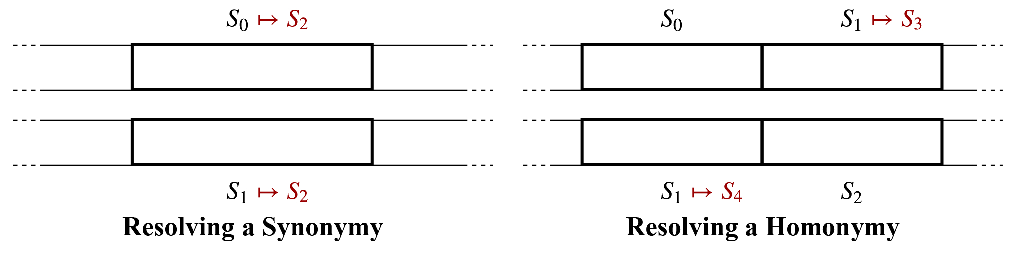
\includegraphics[width=\textwidth]{figs/Lexical.pdf}
    \caption{Caption}
    \label{fig:SolveLexical}
\end{figure}

% The partition is not at fault, the agents just need to change the signs
In the case of a lexical disagreement, the partition made by the two concepts involved in the disagreement are not at fault. The two concepts have a pairing relation of equivalence (homonymy) or are disjoint (synonymy), and the only thing leading them to cause a disagreement is their signs. Therefore, a concept involved in a lexical disagreement is replaced by a concept that share the same intensional and extensional definition, but that has a different sign.

\subsubsection{Resolving Synonymy Disagreements}

% Replace the two synonyms by concepts with a same signs, without touching the other elements
Let $C_{1}$ and $C_{2}$ be two concepts from two agents $A_{1}$ and $A_{2}$, such that their pairing relation in the overall context $U_{O}$ is $C_{i} \equiv_{UO} C_{j}$ and their signs are different: $s(C_{i}) \neq s(C_{j})$. According to Section \ref{sec:SynD}, $C_{i}$ and $C_{j}$ are causing a synonymy disagreement $d_{s}$.
In order to resolve $d_{s}$, each agent $A_{k}$ replaces its concept $C_{k} = \langle s_{k}, I_{k}, E_{k} \rangle$ by a new concept $C'_{k} = \langle s, I_{k}, E_{k} \rangle$. This process is represented in Figure \ref{fig:SolveLexical} (left), where two concepts having different signs $s_{0}$ and $s_{1}$ are replaced by two concepts having the same sign $s_{2}$.
The resulting concepts $C'_{1}$ and $C'_{2}$ are still in a relation of equivalence, since their intensional and extensional definitions remained the same as $C_{1}$ and $C_{2}$, and their signs are now the same. Therefore, according to Section \ref{sec:SynAg}, the pair of concepts $C'_{1}, C'_{2}$ is not causing a disagreement.
As mentioned in Section, \ref{sec:funCreaSign}, the new sign is different from the signs of the overall vocabulary. Therefore, the new concepts cannot cause a homonymy disagreement.

\subsubsection{Resolving Homonymy Disagreements}

% Replace the two homonyms by concepts with different signs, without touching the other elements
Let $C_{1}$ and $C_{2}$ be two concepts from two agents $A_{1}$ and $A_{2}$, such that their pairing relation in the overall context $U_{O}$ is $C_{i} \oslash_{UO} C_{j}$ and they share the same sign: $s(C_{i}) = s(C_{j})$. According to Section \ref{sec:SynD}, $C_{i}$ and $C_{j}$ are causing a homonymy disagreement $d_{s}$.
In order to resolve $d_{h}$, each agent $A_{k}$ replaces its concept $C_{k} = \langle s, I_{k}, E_{k} \rangle$ by a new concept $C'_{k} = \langle s_{k}, I_{k}, E_{k} \rangle$. This process is represented in Figure \ref{fig:SolveLexical} (right), where two concepts having the same sign $s_{1}$are replaced by two concepts having different signs $s_{3}$ and $s_{4}$.
The resulting concepts $C'_{1}$ and $C'_{2}$ are still in a relation of disjunction, since their intensional and extensional definitions remained the same as $C_{1}$ and $C_{2}$, and their signs are now different. Therefore, according to Section \ref{sec:SynAg}, the pair of concepts $C'_{1}, C'_{2}$ is not causing a disagreement.
As mentioned in Section, \ref{sec:funCreaSign}, the two new signs are different from the signs of the overall vocabulary. Therefore, the new concepts cannot cause a synonymy disagreement.

\subsection{Resolving Untranslatable Disagreements}

\begin{figure}[t]
    \centering
    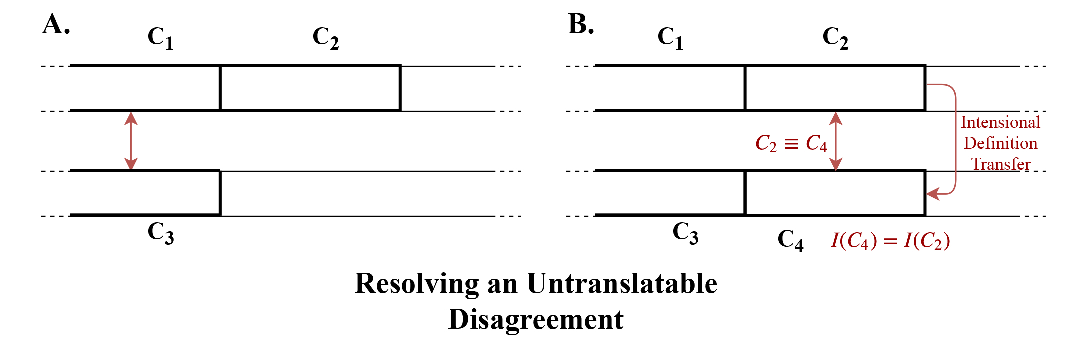
\includegraphics[width=\textwidth]{figs/Untranslatable.pdf}
    \caption{Caption}
    \label{fig:SolveUntrans}
\end{figure}

% One agent needs to create a new concept that is equivalent with the concept of the other agent that does not have an equivalent.
The untranslatable disagreements are a special scenario, as they are not involving two concepts, but one concept and the absence of its equivalent in the other contrast-set. Therefore, an untranslatable disagreement is not resolved by removing a concept but by creating a new one, equivalent to the concept that has no equivalent.
Let $C = \langle s, I, E \rangle$ a concept of the agent $A_{1}$, such that the agent $A_{2}$ has no concept $C'$ in its contrast set such that $C \equiv_{UO} C'$. According to Section \ref{sec:SynD}, this situation results in an untranslatable disagreement $d_{u}$.
In order to resolve $d_{u}$, the agent $A_{2}$ creates a new concept $C' = \langle s, I, Adj(I,U_{2}) \rangle$. Since the two concepts $C$ and $C'$ share their intensional definition -- and thus their adjunct set, they are equivalents according to Definition \ref{def:Relation}.
Now that there exists a concept $C'$ in the contrast-set of $A_{2}$ such that $C \equiv_{UO} C'$, the situation does not cause an untranslatable disagreement anymore.
Since the sign of the concepts $C$ and $C'$ are the same, the two equivalent concepts are not causing a synonymy disagreement.

\subsection{Resolving Self-Disagreements}

\begin{figure}[t]
    \centering
    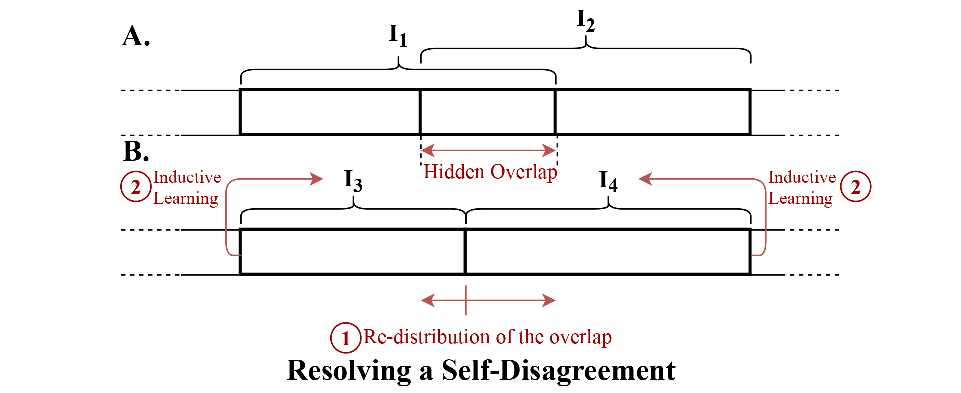
\includegraphics[width=\textwidth]{figs/SelfDisagreement.pdf}
    \caption{Caption}
    \label{fig:SolveSelf}
\end{figure}

% The two concepts are from the same contrast set, only option is that they are in an overall pairing relation of overlap
Let $C_{1}$ and $C_{2}$ two concepts from an agent $A_{1}$ such that $C_{1} \otimes_{UO} C_{2}$. It is important here to note a few things. First of all, since $C_{1}$ and $C_{2}$ belong to a same contrast set, the agent $A_{1}$ cannot see their local pairing relation as $C_{1} \otimes_{U1} C_{2}$, but only as $C_{1} \oslash_{U1} C_{2}$. This means that $A_{1}$ has interacted with another agent $A_{2}$, such that $A_{2}$ has in its local context $U_{2}$ some examples subsumed by both $I(C_{1})$ and $I(C_{2})$.
Moreover, the only pairing relation that can be involved in a self-disagreement is an overlap. Indeed, if $A_{1}$ sees the relation between its two concepts as $C_{1} \oslash_{U1} C_{2}$, this means that there are examples both subsumed by $I(C_{1})$ and not $I(C_{2})$, and examples subsumed by $I(C_{2})$ and not $I(C_{1})$ -- in the local and the overall context. Therefore, the overall pairing relation between $C_{1}$ and $C_{2}$ is either an overlap or a disjunction. Since the signs of the concepts from a same contrast set are all different, the only possible pairing relation causing a disagreement is the overlap. Therefore, a self-disagreement always involves two overlapping concepts.

% Since none of the agent cares to which one of the concept the examples in the overlap should belong to, the agents will use a semantic distance measure that is context independent in order to reassign them
An important specificity of the self-disagreement, is that the examples that are in the overlap of the two concepts have no particular reason to belong to one concept or another. Indeed, the agent $A_{1}$ does not know about these examples, therefore their classification cannot affect its synchronic or diachronic agreement. Moreover, while the agent $A_{2}$ might classify these examples in two or more different concepts, the resulting disagreements should be handled as separate semantic disagreements, not as self-disagreements. For this reason, the two concepts $C_{1}$ and $C_{2}$ should be replaced by a new pair of concepts $C'_{1}, C'_{2}$ such that $C'_{1} \odot_{UO} C'_{2}$ and $Adj(C'_{1},U_{O}) \cup Adj(C'_{2},U_{O}) = Adj(C_{1},U_{O}) \cup Adj(C_{2},U_{O})$.

% Create the new concepts by distributing the examples
The two new concepts will be created through argumentation, one after the other. But the first step for the two agents, is to decide of which sign should be associated to each of the elements from the intersection of $Adj(C_{1},U_{O})$ and $Adj(C_{2},U_{O})$. For now, these examples are associated to both $s(C_{1})$ and $s(C_{2})$, which prevents the creation of a new concept through argumentation. Each agent starts by creating the sets of examples:

\begin{itemize}
    \item $U_{k,C1,\overbar{C2}} = Adj(C_{1},U_{k}) - Adj(C_{2},U_{k})$
    \item $U_{k,C1,C2} = Adj(C_{1},U_{k}) \cap Adj(C_{2},U_{k})$
    \item $U_{k,\overbar{C1},C2} = Adj(C_{2},U_{k}) - Adj(C_{1},U_{k})$
\end{itemize}

% Distances to distribute them
In order to choose, for each example from $U_{1,2,k}$, which sign of $s(C_{1})$ or $s(C_{2})$ is better suited, each agent uses the AU similarity measure. The AU measure quantifies the similarity between an intensional definition $g$ and an example $e$, noted $dAU(g,e)$. Let $I_{1} = \{g_{1,1}, \ldots, g_{1,m}\}$ the intensional definition of $C_{1}$ and $I_{2} = \{g_{2,1}, \ldots, g_{2,n}\}$ the intensional definition of $C_{2}$; For each example $e \in U_{1,2,k}$, $A_{k}$ calculates the average similarities:

\[D_{1} = \frac{1}{|I_{1}|} \times \sum^{m}_{i=1} dAU(g_{1,i},e) \textrm{ and } D_{2} = \frac{1}{|I_{2}|} \times \sum^{n}_{i=1} dAU(g_{2,i},e) \]

% We get a coherent set of associations
Then, $A_{k}$ creates a set of examples $E_{1,k} = \{e \in U_{1,2,k} | D_{1} \geq D_{2} \}$ and a set of examples $E_{2,k} = \{e \in U_{1,2,k} | D_{2} > D_{1} \}$. $A_{k}$ then adds the examples from $U_{1,\overbar{2},k}$ to $E_{1,k}$ and the examples from $U_{\overbar{1},2,k}$ to $E_{2,k}$. Finally, $A_{k}$ associates all the examples of $E_{1,k}$ with $s(C_{1})$ and all the examples of $E_{2,k}$ with $s(C_{2})$. Since the examples of $U_{1,2,k}$ have been re-distributed, the set of associations $E_{1,k} \mapsto s(C_{1}) \cup E_{2,k} \mapsto s(C_{2})$ is coherent. Moreover, since the agents have both access to the intentional definitions $I_{1}$ and $I_{2}$, an example $e$ that is present in both $U_{1,2,1}$ and $U_{1,2,2}$ will have the same associated distances $D_{1}$ and $D_{2}$ independently of the agent that measures them. For this reason, if the example $e$ is put in the set $E_{1,x}$ by $A_{1}$, it will be put in the set $E_{2,x}$ by $A_{2}$ and therefore associated to a same sign. For this reason, the set of associations $E_{1,1} \mapsto s(C_{1}) \cup E_{1,2} \mapsto s(C_{1}) \cup E_{2,1} \mapsto s(C_{2}) \cup E_{2,2} \mapsto s(C_{2})$ is also coherent, authorizing the agents to learn new concepts through argumentation.

% Learning a belief, they arguing
The new concepts $C'_{1}$ and $C'_{2}$ are created through argumentation, sequentially. The agents will start by creating the new concept $C'_{1}$ that will replace $C_{1}$. Following the protocol described in Section \ref{sec:funLeadArg} will lead to the agent $A_{1}$ supervising the creation of $C'_{1}$. $A_{1}$ will therefore create a new belief $\alpha_{1}$ using the set of examples $E_{1,1}$ as a set of positive examples. $A_{2}$ will evaluate this belief using $E_{2,1}$ as the set of positive examples, and eventually argue with $A_{1}$ until it eventually accepts a belief $\alpha' = \langle +, I'_{1}, A_{1} \rangle$. Once the belief is accepted, $A_{1}$ creates the new concept $C'^{1}_{1} = \langle s(C_{1}), I'_{1}, E_{1,1} \rangle$ and replaces $C_{1}^{1}$ with it in its contrast set. Similarly, $A_{2}$ creates a new concept $C'^{2}_{1} = \langle s(C_{1}), I'_{1}, E_{2,1} \rangle$ and replace $C^{2}_{1}$ with it in its hypothesis. Adopting the same strategy for the creation of $C'_{2}$, the agent $A_{1}$ now has a pair of concepts $C'_{1}, C'_{2}$ that are not overlapping in its contrast set.

% They could use other techniques, like distributing every example randomly; making sure that the example has no duplicate in the others concept, but doing so would be an unnecessary cost of examples. Point is: we do not care in which concept they go as long as they stop being in both
Of course, the re-distribution of the examples that are belonging to both the adjunct set $Adj(C_{1},U_{O})$ and the adjunct set $Adj(C_{2},U_{O})$ could be different. Each example $e$ could be randomly assigned to one of the two new concepts $C'_{1}$ and $C'_{2}$, however this would force the agent $A_{k}$ associating $e$ with the sign $s(C_{k})$ to send the association $e \mapsto s(C_{k})$ to the other agent, thus increasing the number of examples exchanged. Without exchanging $e$, the two agents would risk that $A_{-k}$ also has the example $e$ in its contrast-set, and associates it with another sign $s(C_{-k})$. This would result into an non-consistent set of associations on which to build the new intensional definitions upon, which is not possible according to Section \ref{sec:funCreaConA}.

\subsection{Resolving Semantic Disagreements}
\label{sec:ResSemDis}

% Semiotic disagreements are solved through refinement. Concepts involved in semantic disagreements are replaced by their hyponyms
Semiotic disagreements are resolved through the refinement of pre-existing concepts, which means that the concepts involved in a semantic disagreements will either be removed from the contrast set or replaced by a set of co-hyponyms that are partitioning the examples of the concepts involved in the disagreement.

\subsubsection{Resolving Indistinguishable disagreements}

The indistinguishable disagreement is a particular type of example that can only appear if the model admits an error threshold $\tau_{E}$. The notion of error threshold is presented later in Chapter \ref{ErrorManagement}. An error threshold changes the pairing function of our model to neglect non-empty partial sets of comparatively small sizes during the computation of r-triplets. If two newly created concepts $C_{1}$ and $C_{2}$ both have adjunct sets such that $Adj(C_{1}, U_{O}) \geq \tau_{E}$ and $Adj(C_{2}), U_{O} \geq \tau_{E}$ but:

\begin{itemize}
    \item $U_{O,C_{1},C_{2}} < \tau_{E}$ and
    \item $U_{O,\overbar{C_{1}},C_{2}} < \tau_{E}$ and
    \item $U_{O,C_{1},\overbar{C_{2}}} < \tau_{E}$
\end{itemize}

then, the two concepts are considered to be too close from equivalence and one should be removed. The agents resolve the indistinguishable disagreement by removing the concept $C \in \{C_{1}, C_{2}\}$ with the smallest adjunct set $Adj(C, U_{O})$ from the concerned contrast sets. Since $C$ is removed from the argumentation, the disagreement caused by the relation between $C_{1}$ and $C_{2}$ is resolved. This resolution causes a loss in the example coverage of the final contrast set.

\begin{figure}[t]
    \centering
    \includegraphics[width=\textwidth]{figs/Semantic.pdf}
    \caption{Caption}
    \label{fig:SolveSemantic}
\end{figure}

\subsubsection{Resolving Hypo/Hypernymy disagreements}

Let $C_{1} \in S_{1}$ and $C_{2} \in S_{2}$ be two concepts from two agents $A_{1}$ and $A_{2}$, such that their pairing relation in the overall context $U_{O}$ is $C_{1} \odot_{UO} C_{2}$, and let $C_{1}$ be the hypernym of $C_{2}$. According to Section \ref{sec:SynD}, $C_{1}$ and $C_{2}$ are causing a hypo/hypernymy disagreement $d_{h}$.
% Splitting in two co-hyponyms.
In order to resolve $d_{h}$, $A_{1}$ will delete $C_{1}$ from $S_{1}$ and replace it by $C_{3}$, the co-hyponym of $C_{2}$ with regard to $C_{1}$. This process is represented in Figure \ref{fig:SolveSemantic}. The agents use argumentation in order to create $C_{3}$ such that $I(C_{3})$ is best to subsume $Adj(C_{3}, U_{O}) = U_{C1,\overbar{C2},O}$. Since $C_{1}$ is removed from $S_{1}$, the disagreement $d_{h}$ is resolved. However, the overall pairing relations between $C_{3}$ and others concept is unknown except for $C_{2}$.
% In Boolean model, fine because of property 3
If we do not admit an error threshold, we can prove through Property \ref{pp:} that the pairing relation between $C_{3}$ and any other concept is a disjunction, which can only lead to a lexical disagreement (homonymy). If an error threshold is present in the model, the creation of $C_{3}$ can cause further disagreements.

\subsubsection{Resolving Overlap disagreements}

Let $C_{1}$ and $C_{2}$ be two concepts from two agents $A_{1}$ and $A_{2}$, such that their pairing relation in the overall context $U_{O}$ is $C_{1} \otimes_{UO} C_{2}$. According to Section \ref{sec:SynD}, $C_{1}$ and $C_{2}$ are causing an overlap disagreement $d_{o}$.
% Creating a hyponym for the examples in the overlap, resulting in two hypo/hypernym disagreements.
In order to resolve $d_{o}$, $A_{1}$ and $A_{2}$ will both add a concept $C_{3}$ that is the hyponym of both $C_{1}$ and $C_{2}$ to their contrast sets. The agents use argumentation in order to create $C_{3}$ such that $I(C_{3})$ is best to subsume $Adj(C_{3}, U_{O}) = U_{C1,C2,UO}$. Since neither $C_{1}$ nor $C_{2}$ is removed from the agents contrast sets, the disagreement $d_{o}$ is \emph{not} resolved.

However, at least two new disagreements appeared. Since $C_{3}$ is a hyponym of both $C_{1}$ and $C_{2}$, we have $C_{1} \odot_{UO} C_{3}$ and $C_{2} \odot_{UO} C_{3}$. According to Section \ref{sec:SynD}, $C_{1} \odot_{UO} C_{3}$ causes a hypo/hypernymy disagreement $d_{h1}$ and $C_{2} \odot_{UO} C_{3}$ causes a hypo/hypernymy disagreement $d_{h2}$. Since resolving each disagreement $d_{hx}$ involves removing the concept $C_{x}$ as it is a hypernym, the disagreement $d_{o}$ will be resolved upon resolution of $d_{h1}$ and $d_{h2}$.

% In Boolean model, fine because of property 3

 

\chapter{Inductive Learning Error Management}\label{ErrorManagement}
\section{General Idea}
\label{sec:DoGGenIdea}

Among the three semiotic elements of the concept, the intensional definition stands aside. Unlike the two other semiotic elements -- the sign and the extensional definition -- the intensional definition is not initially  present in the data used by the agents to create concepts: it is the element that has to be learned. The intensional definition is created by the agent through inductive learning, which means that it can suffer from some of the limitations that are frequently encountered in machine learning. Each intensional definition is an attempt at a binary classification (see Section \ref{sec:funCreaConA}), and this classification suffers from two limitations associated with every machine learning classifiers:

\begin{enumerate}
    \item it requires a certain number of positive and negative examples to be able to learn, and
    \item it is likely to produce false positives and negatives
\end{enumerate}


More generally, we discussed in Section \ref{sec:funCreaConE} that when an agent creates a concept $C$ from right-path associations, it needs a class $U(\mapsto s)$ and its associated sign $s$. In order to be able to use inductive learning, the number of examples in the class $U(\mapsto s)$ should be above a certain threshold. We will call this threshold $\tau_{1}$. Upon learning the new concept $C$ from the right-path associations $U \mapsto s$, the set of examples $U(\mapsto s)$ should become the extensional definition of $C$, admitting that the classification ended with an accuracy of 1. Therefore, since $U(\mapsto s) \geq \tau_{1}$, the extensional definition $E(C)$ is expected to have at least $\tau_{1}$ examples. Therefore, during their argumentation, the agents should not consider possible to have concepts that are expected to have less than $\tau_{1}$ examples -- and moreover they should never try to create a such concept. This remark collides with the fact the until now, agents can consider pairing partial sets with a minimum of one example as non empty which can cause them to try to create concepts for these partial sets. This can for instance be the case during the resolution of a semantic disagreement, as we discussed in Section \ref{sec:Resolution}.

The situation described in the paragraph above assumes that the inductive learning can be achieved with an accuracy of 1, which is, as we mentioned earlier, unlikely to happen -- especially because one agent is expected to have access to only roughly half of the examples of the overall contrast set during the right-path association learning of one of its initial concepts, which cannot guarantee a good accuracy over the other half of the overall context. 

Let $A_{1}$ and $A_{2}$ be two agents. Each agent receives an equal and homogeneous partition of a set of left-path associations $U \mapsto S = \{s \ldots s_{n} \}$. Each agent $A_{k}$ tries to learn a new concept $C_{k} = \langle s, I_{k}, E_{k} \rangle$. The intensional definition $I_{1}$ learned by the agent $A_{1}$ is likely to either not subsume examples of $A_{2}$'s context that $A_{2}$ associates with $s$ (first-type error), or to subsume examples from $A_{2}$'s context that $A_{2}$ does not associate with $s$ (second-type error). That's why upon receiving $I_{1}$ and building a copy of $C_{1}$ in its hypothesis, $A_{2}$ cannot assume that the examples of $U_{2,C1,\overbar{C2}}$ and $U_{2,\overbar{C1},C2}$ are examples from a non-equivalent concept of $A_{1}$ as it should be the case with the pairing function presented in Section $\ref{sec:Relations}$. The agents need to decide of a threshold $\tau_{2}$ for the first-type error, and a threshold $\tau_{3}$ for the second-type error, under which the agents assume that the size of a pairing partial set is not indicative of any hidden concept, but of a lack of accuracy from the inductive learning instead.

Instead of having three different thresholds, we chose to regroup them in one error threshold since they all aim to change the same thing: the minimal amount of examples in a pairing partial set for it to not be considered as empty. This unique threshold $\tau_{E}$ is the highest from the expected $\tau_{1}$, $\tau_{2}$ and $\tau_{3}$. In our scenarios and experiments, this threshold $\tau$ is given as a parameter to both agents before the communication starts. While it is probably possible to grant the multi-agent system the ability to find the optimal value for $\tau$ by itself, this is not the object of this thesis and we will not discuss it. In the general case where concepts from a same contrast set have roughly the same number of examples, $\tau_{2}$ and $\tau_{3}$ are expected to be inferior to $\tau_{1}$ -- the size of a concept should be greater than the first-type and second-type errors, otherwise the classifier's performances are so poor that it should not be use in the first place -- and therefore $\tau = \tau_{1}$ in most practical cases.

There are two immediate points that can be noticed on the error threshold. The first is that the error threshold cannot be inferior to one, as an error threshold of zero or less would imply that pairing partial sets considered as empty have a negative cardinality, which is strictly impossible in our model. The second is that with an error threshold $\tau = 1$, our model remains as it was before the introduction of the error threshold. An empty set is a set with no example, an any number of example above one results in the set being considered as non-empty.

At this point, it is important to emphasis the fact that we consider the pairing partial sets to be empty if their cardinality is under the threshold $\tau$ purely from the point of view of our pairing function. The empty set $\emptyset$ still remains a set with a 0 cardinality. However, two concepts $C_{1}$ and $C_{2}$ such that:

\begin{itemize}
    \item $U_{O,C1,C2} < \tau$
    \item $U_{O,\overbar{C1},C2} < \tau$
    \item $U_{O,C1,\overbar{C2}} \geq \tau$
\end{itemize}

will now be considered as equivalent such that $C_{1} \equiv_{UO} C_{2}$, as if $U_{O,\overbar{C1},C2}$ and $U_{O,C1,\overbar{C2}}$ were empty while using our initial pairing function.

The introduction of the error threshold, and the evolution that it induces in the notion of equivalence between concepts, requires the modifications of several definitions. An implementation of our model with the definitions below and an error threshold $\tau > 1$ is referred as an integer-triplet model, since the r-triplets will now store the cardinality of the pairing partial sets instead of "0" for empty and "1" for non-empty. On the contrary, an implementation of our model with the definitions presented in Chapter \ref{Approach} is referred as a boolean-triplet model, since the r-triplets store "1" and "0" as boolean variables for the truthiness of the proposition: \emph{my corresponding pairing partial set is non-empty}.

\section{Effect on Semiotic Elements and Containers}
\label{sec:DoGEffectCon}

In Definition \ref{def:Con}, we stated that for any concept $C = \langle s, I, E \rangle$ we should have the equality $E = X$ where $X = \{ e \in U | I \sqsubseteq e \}$. If the concept $C$ has been created from left-path associations, this definition is not problematic as: 

\begin{itemize}
    \item $E \Leftrightarrow Adj(I,U)$
    \item $\Leftrightarrow \{ e \in U | I \sqsubseteq e \}$
    \item $\Leftrightarrow X$
\end{itemize}

The equality $E = X$ is maintained and our definition still stand. However, if the concept is created from right-path associations or through argumentation, the situation is different. In each of these two situations, the extensional definition $E$ of the created concept is the subset $U_{+} \subset U$ that served as the positive examples during the inductive learning. As we now admit a certain degree of error during our inductive learning, the introduction of $\tau$ should be reflected in the relation between $E$ and $U_{+}$ that should no longer have to be an equality.

A solution would be to modify the equality $E = X$ in the definition of concepts, but we prefer to actually modify the creation process of our concepts, in order to keep the equality $E = X$ and prioritize the left-path associations over the right-path associations in our model. If the model admits an error threshold $\tau > 1$, any concept created in a context $U$ should have its extensional definition $E$ be $E = Adj(C_{i}, U)$.

However, the decision to keep $E = X$ impacts directly the contrast sets, that cannot be longer strict partitions. Given the consistent set of right-path associations $U \mapsto S$, such that $S = \{s_{1}, \ldots, s_{n} \}$; if an agent $A$ learns a concept $C_{i}$ for each class $U(\mapsto s_{i})$ with $s_{i} \in S$, then we can now tolerate that 1) $I(C_{i})$ subsumes $\tau_{E}$ examples that are belonging to another class $U(\mapsto s_{j})$, and 2) not subsume $\tau$ examples that are belonging to $U(\mapsto s_{i})$. While the fact that $U \mapsto S$ is consistent means that $(U, \{ C(s_{i}) | s_{i} \in S \})$ should be a contrast set if the inductive learning takes place with a maximal accuracy during the creation of each $C_{i}$, this is not the case if the learning admits a degree of error $\tau_{E}$. Actually, if both $C_{i}$ and $C_{j}$ have bean created with a first-type error of $\tau$, the overlap $E_{i} \cap E_{j}$ can reach $2 \times \tau$. We will note $\tau_{E} = 2 \times \tau$. If we want $(U, \{ C(s_{i}) | s_{i} \in S \})$ to be a contrast set, we must change our definition of a contrast set such that:

\begin{itemize}
    \item regarding the first point, the intersection between two extensional definitions of two different concepts can be non-empty as long as it is not above the threshold $\tau_{E}$, and
    \item regarding the second point, we cannot longer guarantee that $E_{1} \cup \ldots \cup E_{n} = U$.
\end{itemize}

Taking these two limitations into account, we can now give a new definition to contrast sets, Definition \ref{def:CsetDoE}. This definition will replace Definition \ref{def:Cset} in implementations that use an integer-triplet model.

\begin{restatable}[Contrast Set With Degree of Error]{df}{contrastSetDoE}
\label{def:CsetDoE}
A contrast set $K = (U_{K}, S_{K} = \{ C_{1}, \ldots ,C_{n} \})$ is a container. For each pair of concepts $C_{i}, C_{j} \in S_{K}$, we should have the following property: $|E(C_{i}) \cap E(C_{j})| < \tau_{E}$. Moreover, the signs of the concepts must be different: $\forall C_{i},C_{j} \in K$, $i \neq j \Rightarrow s(C_{i}) \neq s(C_{j})$.
\end{restatable}

The other container, the hypothesis, does not tackle the issue of overlapping extensional definitions and never aimed to be a partition. Since no relation between sets of examples were required in the hypothesis, the modification to the definition of concept does not affect the definition of hypotheses.

\section{Effect on Relations Between Concepts}
\label{sec:DoGEffectRelation}

A field that is extensively affected by the introduction of an error degree is the relation between concepts. We will move from the idea that $\tau$ as an element of a binary classification to go back to the idea of an error tolerance in order for two concepts to remain equivalents in a context. We move from a model where the equivalence between two concepts $C_{1}$ and $C_{2}$ in a context $U$ is defined by $Adj(C_{1}, U) = Adj(C_{2}, U)$ and thus $| Adj(C_{1}, U) \triangle Adj(C_{2}, U)| = 0$, to a model where the equivalence between $A$ and $B$ is defined by $|Adj(C_{1}, U) \triangle Adj(C_{2}, U)| < \tau_{E}$.

\subsection{Assuming a Degree of Error in R-Triplets}
\label{sec:LPRassumingDoG}

The first step to evaluate the relation between two concepts $C_{i}$ and $C_{j}$ in a context $U$ was to find their pairing partial sets, as presented in Section \ref{sec:PPSet}. These pairing partial sets were allowing us to find the r-triplet of $C_{i}$ and $C_{j}$ in $U$, but the definition of r-triplets was based on whether or not the partial sets were empty. Replacing the notion of set emptiness with the notion of set cardinal inferior to a threshold, we substitute Definition \ref{sec:PPSet} by Definition \ref{def:RTripletDoG} below:

\begin{restatable}[R-Triplet Function with Degree of Error]{df}{rTripletDoG}
\label{def:RTripletDoG}
The function $r: \mathbb{X} \times \mathbb{X} \times \mathbb{U} \rightarrow  \mathbb{N}^{3}$, with $\mathbb{X}$ the domain of concepts and $\mathbb{U}$ the domain of all possible contexts, is a function that for each pair of concepts $C_{i}$,$C_{j}$ and for a given context $U$ yields a triplet $(b_{-1},b_{0},b_{1})$ called r-triplet accordingly to the definition below:

\begin{itemize}
\item $b_{-1} = \left\{
	\begin{array}{ll}
		0  & \mbox{if } |U_{C_i,\overbar{C}_j}| < \tau \\
		1 & \mbox{otherwise}
	\end{array}
\right.$
\item $b_{0} = \left\{
	\begin{array}{ll}
		0  & \mbox{if } |U_{C_i,C_j}| < \tau \\
		1 & \mbox{otherwise}
	\end{array}
\right.$
\item $b_{1} = \left\{
	\begin{array}{ll}
		0  & \mbox{if } |U_{\overbar{C}_i,C_j}| < \tau \\
		1 & \mbox{otherwise}
	\end{array}
\right.$
\end{itemize}
\end{restatable}

Using the r-triplet function defined in Definition \ref{def:RTripletDoG} with the Definition \ref{def:Relation} to find pairing relations between concepts results in more indulgent pairing relations. Small overlaps between concepts do not necessarily results into concepts not being equivalents. In this configuration, we say that our pairing relations are assuming a degree of error $\tau_{E}$. While a simple substitution of Definition \ref{def:RTriplet} by Definition \ref{def:RTripletDoG} can work as a simplified model, it is theoretically incorrect as we will now demonstrate.

\subsection{Problem with Inferring Overall R-Triplets}

Simply substituting Definition \ref{def:RTriplet} by Definition \ref{def:RTripletDoG} in our model is incorrect, since Theorem \ref{thm:Overall} does not held with r-triplets defined by Definition \ref{def:RTripletDoG} as stated in Proposition \ref{pp:ImpOverall}. This means that our changes to the definition of r-triplets are preventing the inference of overall r-triplets from local ones. The inference of overall r-triplets by local ones being a key function of our argumentation model, further modifications of the definition of r-triplets are required. These modifications should allow to both: assume a degree of error for our pairing relations, and infer overall triplets from the local ones.

\begin{restatable}[Impossibility to Infer Overall Pairing Relation]{prp}{ImpOverall}\label{pp:ImpOverall}
Let $A_{1}$ and $A_{2}$ be two  agents, $A_{1}$ partitioning the context $U_{1}$ in the contrast set $K_{1} = \{ U_{1}, S_{1} \}$ and $A_{2}$ partitioning the context $U_{2}$ in the contrast set $K_{2} = \{ U_{2}, S_{2}\}$. Let $C_{i} \in S_{1}$ and $C_{j} \in S_{2}$ be two concepts, and

\begin{itemize}
%\item the two local triplets:
%\begin{itemize}
\item let $r(C_{i},C_{j},U_{1}) = (b_{-1}, b_{0}, b_{1})$ be the local triplet of $A_{1}$
\item let $r(C_{i},C_{j},U_{2}) = (b'_{-1}, b'_{0}, b'_{1})$ be the local triplet of $A_{2}$
%\end{itemize}
\item  let $r(C_{i}, C_{j}, U_{O}) = (b''_{-1}, b''_{0}, b''_{1})$ be the overall triplet $A_{1}$ and $A_{2}$
\end{itemize}

While using Definition \ref{def:RTripletDoG} to define r-triplets instead of \ref{def:RTriplet} and for any $n \in \{-1, 0, 1\}$, the fact that $b_{n} = 0$ and $b_{n}' = 0$ does not necessarily mean that $b_{n}'' = 0$.
\end{restatable}

\begin{proof}
See Appendix \ref{ap:2}.
\end{proof}

\subsection{Finding Overall R-Triplets in Integer-Triplet Models}

In order to go through this issue, there is a necessity to differentiate the aim of \emph{local} r-triplets and \emph{overall} r-triplets. While computing pairing partial sets and r-triplets, the agents' final goal is to find the overall r-triplet of a pair of concepts that will give away the overall pairing relation between these two concepts. The local r-triplets are just a transitory step to help the agents finding the overall r-triplets without having to exchange their whole contexts.

When the model admits a degree of error, the agents will need more transitory steps to determine their overall pairing relations. This will be reflected by new types of r-triplet that represent new steps of the transition between local pairing partial sets and overall pairing relations. The last type of r-triplet should be the same as the input of the pairing function presented in \ref{sec:Relations}, that associates each possible triplet of booleans to a type of pairing relation.

\subsubsection{Local R-Triplets}

% local r-triplets
Let $A_{1}$ and $A_{2}$ be two  agents, $A_{1}$ partitioning the context $U_{1}$ in the contrast set $K_{1} = \{ U_{1}, S_{1} \}$ and $A_{2}$ partitioning the context $U_{2}$ in the contrast set $K_{2} = \{ U_{2}, S_{2}\}$. Let $C_{i} \in S_{1}$ and $C_{j} \in S_{2}$ be two concepts. In order to find the pairing relation between two concepts $C_{i}$ and $C_{j}$, the first step that the two agents can take is to find their local r-triplets. However, the local r-triplets need to carry more information than what is defined in Definition \ref{def:RTripletDoG}, as we have shown through Proposition \ref{pp:ImpOverall} that local boolean r-triplets were useless to infer overall the r-triplet. For this reason, the local r-triplets are now using integers. These integer values represent the size of their associated pairing partial sets, and will help the agents to determine the sizes of the different overall pairing partial sets. Once the sizes of the different overall pairing partial sets have been determined, the agents can find which overall pairing partial set contains $\tau$ examples or more, and therefore associate an overall pairing relation to $C_{i}$ and $C_{j}$ which acknowledge an error degree. These local r-triplets of our integer-triplet model are presented in Definition \ref{def:lRTriplet} below:

\begin{restatable}[Local R-Triplet]{df}{lRT}
\label{def:lRTriplet}
The function $r_{l}: \mathbb{X} \times \mathbb{X} \times \mathbb{U} \rightarrow  \mathbb{N}^{3}$, with $\mathbb{X}$ the domain of concepts and $\mathbb{U}$ the domain of all local contexts, is a function that for each pair of concepts $C_{i}$,$C_{j}$ and for a given context $U$ yields a triplet $(i_{-1},i_{0},i_{1})$ called local r-triplet accordingly to the definition below:

\begin{itemize}
\item $i_{-1} = \left\{
	\begin{array}{ll}
		|U_{C_i,\overbar{C}_j}|  & \mbox{if } |U_{C_i,\overbar{C}_j}| < \tau \\
		\tau & \mbox{otherwise}
	\end{array}
\right.$
\item $i_{0} = \left\{
	\begin{array}{ll}
		|U_{C_i,C_j}|  & \mbox{if } |U_{C_i,C_j}| < \tau \\
		\tau & \mbox{otherwise}
	\end{array}
\right.$
\item $i_{1} = \left\{
	\begin{array}{ll}
		|U_{\overbar{C}_i,C_j}|  & \mbox{if } |U_{\overbar{C}_i,C_j}| < \tau \\
		\tau & \mbox{otherwise}
	\end{array}
\right.$
\end{itemize}
\end{restatable}

\subsubsection{Loose R-Triplets}

% overall loose r-triplets
In the boolean-triplet model, the agents could combine their local r-triplets to find an overall r-triplet. From the overall r-triplet, the agents could know which overall pairing partial sets were empty and which were not. In a model that assumes a degree of error, the agents do not aim to find which overall pairing partial sets are empty but which overall pairing partial sets contain less than $\tau$ examples. From their two local r-triplets, the agents can infer some values of the overall r-triplet, but some other values will remain unknown for the moment. An overall r-triplet that contains unknown values is an overall \emph{loose} r-triplet. Loose r-triplets cannot be used to find the overall pairing relation between $C_{i}$ and $C_{j}$ directly, but remains a good starting point. The overall loose r-triplets of two local r-triplets is defined below in Definition \ref{def:olRTriplet}:

\begin{restatable}[Overall Loose R-Triplet]{df}{olRT}
\label{def:olRTriplet}
The function $r_{ol}: \mathbb{N}^{3} \times \mathbb{N}^{3} \rightarrow  \mathbb{N}^{3}$ is a function that for each pair of r-triplet $(i'_{-1}, i'_{0}, i'_{1})$, $(i''_{-1}, i''_{0}, i''_{1})$ yields a triplet $(i_{-1},i_{0},i_{1})$ called overall loose r-triplet accordingly to the definition below:

\begin{center}
    $i_{n} = \left\{
	\begin{array}{lll}
		\tau & \mbox{if } i'_{n} \geq \tau \mbox{ or } i''_{n} \geq \tau \\
		0    & \mbox{if } i'_{n} + i''_{n} < \tau \\
		? & \mbox{otherwise}
	\end{array}
\right.$
\end{center}

\end{restatable}

If loose r-triplets are a good intermediary step to find the overall r-triplet, it is because it already gives some partial information on which overall pairing partial sets contain more than $\tau$ examples. This property of the loose r-triplets is explained in Property \ref{pp:olUseful}.

\begin{restatable}[Loose R-Triplet Usefulness]{pp}{olUseful}
\label{pp:olUseful}
Let $A_{1}$ and $A_{2}$ be two  agents, $A_{1}$ partitioning the context $U_{1}$ in the contrast set $K_{1} = \{ U_{1}, S_{1} \}$ and $A_{2}$ partitioning the context $U_{2}$ in the contrast set $K_{2} = \{ U_{2}, S_{2}\}$. Let $C_{i} \in S_{1}$ and $C_{j} \in S_{2}$ be two concepts, and let $r_{1}$ and $r_{2}$ be two local r-triplets such that:

\begin{itemize}
    \item $r_{1} = r_{l}(C_{i}, C_{j}, U_{1})$, and
    \item $r_{2} = r_{l}(C_{i}, C_{j}, U_{2})$.
\end{itemize}

For each value $i_{n}$ from the triplet $r_{ol}(r_{1},r_{2})$, its associated pairing partial set $U_{O}(n)$ contains less than $\tau$ examples if an only if $i_{n} = 0$, and contains at least $\tau$ examples if and only if $i_{n} = \tau$.
\end{restatable}

\begin{proof}
See Appendix \ref{}.
\end{proof}

\subsubsection{Secured R-Triplets}

% overall secured r-triplets
Once the agents have computed the loose r-triplets, they need to attribute an integer to the elements of unknown values. The next step for the agent is to produce a r-triplet that implements Property \ref{pp:olUseful}, but without any unknown value. Since according to Property \ref{pp:olUseful} the unknown value $i_{n}$ of a loose triplet $r$ should be (1):

\begin{itemize}
    \item 0 if and only if $|U_{O}(n)| < 0$, and
    \item $\tau$ if and only if $|U_{O}(n)| \geq 0$,
\end{itemize}

then the agents can find each unknown value by $i_{n}$ accessing the corresponding pairing partial set $U_{O}(n)$. In Section \ref{sec:Overall}, we mentioned that the overall pairing partial set $U_{O}(n)$ is the union of the two local pairing partial sets $U_{1}(n)$ and $U_{2}(n)$. The issue is that each local pairing partial set $U_{k}(n)$ is a subset of the local context $U_{k}$ of the agent $A_{k}$, and is supposed to be accessed only by $U_{k}$. However, we saw in Section \ref{sec:funMessages} that an agent can choose to share examples with the other, by sending a message \emph{Examples()}. It is therefore possible for an agent $A_{k}$ to access an overall pairing partial set $U_{O}(n)$, as long as the other agent $A_{-k}$ sends the examples $U_{-k}(n)$ to $A_{k}$.

Upon accessing an overall pairing partial set $U_{O}(n)$ that is associated an to unknown value $i_{n}$ of a loose r-triplet, an agent can compute an overall \emph{secured} r-triplet of this loose r-triplet, where the unknown value $i_{n}$ is \emph{secured} -- replaced by a known value -- by adding information from an external set of examples $U^{*}$. The notion of secured r-triplet is defined below in Definition \ref{def:osRTriplet}.

\begin{restatable}[Overall Secured R-Triplet]{df}{osRT}\label{def:osRTriplet}

The function $r_{os}: \mathbb{N}^{3} \times \mathbb{U} \rightarrow  \mathbb{N}^{3}$, with $\mathbb{U}$ being the domain of all sets of examples, is a function that, for a loose r-triplet $(i'_{-1}, i'_{0}, i'_{1})$ and a given set of example $U*$, yields a triplet $(i_{-1},i_{0},i_{1})$ called overall secured r-triplet accordingly to the definition below:

\begin{center}
    $i_{n} = \left\{
	\begin{array}{lll}
		i'_{n} & \mbox{if } i'_{n} \mbox{ is known }  \\
		U^{*}(n) & \mbox{otherwise } \\
	\end{array}
\right.$
\end{center}

\end{restatable}

Secured r-triplets are useful for multiple reasons. Ultimately, they are the first presented r-triplets that can achieve the goal that we set: under the right conditions, they can indicate which overall pairing partial sets contain $\tau$ examples or more and which does not. As we mentioned at the beginning of this section, the function $r_{os}$ replaces an unknown value $i_{n}$ of a loose r-triplet $r = r_{ol}(C_{i}, C_{j}, U_{O})$ by a known value $i'_{n}$ that is equal to:

\begin{itemize}
    \item 0 if and only if $|U_{O}(n)| < 0$, and
    \item $\tau$ if and only if $|U_{O}(n)| \geq 0$,
\end{itemize}

as long as $r_{os}$ takes as input parameters the triplet $r$ and \emph{any} super-set of $U_{O}(n)$. This property is formalized below in Property \ref{pp:slUseful}.

\begin{restatable}[Secured R-Triplet Usefulness]{pp}{slUseful}
\label{pp:slUseful}

\end{restatable}

\begin{proof}
See Appendix \ref{}.
\end{proof}

This means that if a loose r-triplet $r$ contains two missing values $i_{m}$ and $i_{n}$, the secure r-triplet  $r_{os}(r,$ $U_{1}(m)$$\cup$$U_{1}(n)$$\cup$$U_{2}(m)$$\cup$$U_{2}(n))$ results in a triplet with no unknown value, and where each r

Moreover, secured r-triplets that have unknown values of different indexes can be combined to 

\subsubsection{Binarized R-Triplet}

% overall binarized r-triplets
Once an agent has found the overall secured r-triplet $r_{os}$ for the pair of concepts $C_{i}, C_{j}$, it still needs to transform this triplet of integers into a triplet of booleans. The triplet $r_{os}$ can only contain zeros and $\tau$s, therefore the agent replaces each value $i_{x}$ of $r_{os}$ that are equal to $\tau$ by 1 and obtain a triplet of booleans. We call this final triplet the overall \emph{binarized} r-triplet, noted $r_{ob}$. The binarized triplet can be used along with the pairing function presented in Definition \ref{def:Relation} to find the overall pairing relation between $C_{i}$ and $C_{j}$. Recall that since Theorem \ref{thm:ROverall} was deduced from Theorem \ref{thm:Overall}, and since Theorem \ref{thm:Overall} has been invalidated in the integer-triplet model, therefore Theorem \ref{thm:ROverall} is also invalidated. The definition of binarized r-triplet is presented below in Definition \ref{def:bRTriplet} is compliant with the definition of r-triplets given in Definition \ref{def:RTripletDoG}.

\begin{restatable}[Binarized Overall R-Triplet]{df}{bRT}\label{def:bRTriplet}

\end{restatable}

\subsubsection{Optimization}
% Case of same-size local pairing partial sets
If we follow the method described in the above paragraphs, an unknown value $i_{x}$ from the loose r-triplet $r_{ol}(C_{i},C_{j},U_{O})$ pushes each agent $A_{k}$ to send its pairing partial set $U_{k,x}$ to the other agent in the case where $|U_{1,x}| = |U_{2,x}|$. In this situation, we call the unknown value $i_{x}$ a \emph{draw} value. This increases the number of example exchanged when only one of these two pairing partial sets needs to be exchanged. Since the argumentation protocol is turn-based, the agents can bypass this issue by knowing if one of the two pairing partial sets $U_{1,x}$ or $U_{2,x}$ has already been exchanged when it is their turn to send one of them. If it is the case, the agent do not need to send a redundant information as one of the two pairing partial set will already already be accounted for in both semi-secured r-triplets.

\subsection{Example of Overall Pairing Relation Retrieving}

% Example
In order to illustrate how two agents can determine the overall pairing relation between two of their concepts, we propose the following scenario. Let $A_{1}$ and $A_{2}$ be two agents, with $A_{1}$ having a contrast set $K_{1} = \{S_{1}, U_{1} \}$ and $A_{2}$ having a contrast set $K_{2} = \{S_{2}, U_{2}\}$. Let $C_{1}$ and $C_{2}$ be two concepts such that $C_{1} \in S_{1}$ and $C_{2} \in S_{2}$. The agents are in an argumentation where they admit that a degree of error $\tau = 10$ is possible. Admitting that $A_{1}$ and $A_{2}$ have both access to $s(C_{1}),s(C_{2})$ and $I(C_{1}), I(C_{2})$, the agents compute their local r-triplets and:

\begin{itemize}
    \item $A_{1}$ finds that $r(C_{1},C_{2}, U_{1}) = (5,12,8)$
    \item $A_{2}$ finds that $r(C_{1},C_{2}, U_{2}) = (4,9,9)$
\end{itemize}

The agents compare each values $i_{k,x}$ of their local r-triplets that share a same index $x \in \{-1,0,1\}$. For $x = 0$, $i_{1,-1}$ is 5 and $i_{2,-1}$ is 4. Their sum is $9$, which is less than $\tau$. Therefore, the overall pairing partial set $U_{O}(i_{-1})$ cannot contain $\tau$ examples, even if $U_{1}(i_{-1}) \cap U_{2}(i_{-1}) = \emptyset$. For $x = 1$, $i_{1,0}$ is 12 and $i_{2,0}$ is 9. Here, the value of $i_{2,0}$ does not matter because the value of $i_{1,0}$ is already above $\tau$. Since:

\begin{itemize}
    \item $U_{1}(i_{0}) \geq \tau$
    \item $\Leftrightarrow U_{1}(i_{0}) \cup U_{2}(i_{0}) \geq \tau$
    \item $\Leftrightarrow U_{O}(i_{0}) \geq \tau$
\end{itemize}

the size of the overall pairing partial set associated to the index $1$ is above $\tau$, and its value should be $\tau$. For $x = 1$, the situation is more complex. Since $i_{1,1}$ is equal to 8 and $i_{2,1}$ is equal to 9, their sum is 17 which means that if $U_{1}(i_{1})$ and $U_{2}(i_{1})$ were disjoint, the overall pairing partial set $U_{O}(i_{1})$ would contain well above $\tau$ examples. However, in the case where $U_{1}(i_{1}) \subset U_{2}(i_{1})$, $U_{O}(i_{1})$ would only contain 9 examples. The agents cannot compare the two local pairing partial sets, as they only share the intensional definitions and signs of the concepts and do not have the same local contexts. The value of $i_{O,1}$ is left undefined in the overall r-triplet. At this point, the agents have computed that the overall r-triplet $r_{O}$ is equal to $(0,\tau,?)$.

In order for one of the two agents $A_{k}$ to compute the actual value of $i_{O,1}$, one of them needs to add the pairing partial set $U_{-k}(i_{1})$ to its context. Thanks to Property \ref{pp:CompUndefinedValue}, $A_{k}$ will be able to compute the value of $i_{O,1}$. Instead of having the two agents sending their examples, the agent that has the least examples in its pairing partial set can send them to the other agent, that will compute $i_{O,1}$ and then share it back. Doing so decreases the number of examples that need to be exchanged between the agents. In our scenario, $A_{1}$ sends the 8 examples of $U_{1}(i_{1})$ to $A_{2}$. Upon receiving them, $A_{2}$ adds $U_{1}(i_{1})$ to its context $U_{2}$. Then, $A_{2}$ observes that the new pairing partial set $U_{2}(i_{1})$ contains 10 elements. $A_{2}$ replaces the undefined value ``?'' in $r_{O}$ by $\tau$. Then, $A_{2}$ can share $r_{O} = (0, \tau, \tau)$ with $A_{1}$.


\section{Effect on the Transitivity of the Equivalence Pairing Relation}
\label{sec:TransitivityLoss}

A relation of equivalence is reflexive, symmetrical and transitive. Before the introduction of an error degree, the pairing relation of equivalence was verifying all of these properties. Indeed, for any concepts $C_{i}$, $C_{j}$ and $C_{k}$:

\begin{itemize}
    \item $C_{i} \equiv C_{i}$,
    \item if $C_{i} \equiv C_{j}$ then $C_{j} \equiv C_{i}$ and
    \item if $C_{i} \equiv C_{j}$ and $C_{j} \equiv C_{k}$, then $C_{i} \equiv C_{k}$.
\end{itemize}

\begin{proof}
See annex \ref{}.
\end{proof}

However, introducing a degree of error means that our relation of equivalence is not transitive anymore. Figure \ref{} illustrates a situation where $C_{1}$ and $C_{2}$ share more than $\tau$ examples, with $C_{1} - C_{2}$ and $C_{2} - C_{1}$ having both less than $\tau$ examples, meaning that $C_{1}$ and $C_{2}$ are equivalents in $U$. The remark is the same for $C_{2}$ and $C_{3}$. However, $C_{1}$ and $C_{3}$ share less than $\tau$ examples and therefore are not equivalents. This means that while $C_{1} \equiv C_{2}$ and $C_{2} \equiv C_{3}$, $C_{1} \not \equiv C_{3}$. The transitivity of our equivalence is lost.

However, the transitivity of the equivalence relation is needed in our model. For instance, two disjoint concepts $C_{1}$ and $C_{2}$ from a same contrast set that are both equivalent to a third concept $C_{3}$ from another contrast set can cause a dead loop in the argumentation. If $C_{1}$ and $C_{2}$ share the same sign, they are homonyms and cause a homonymy disagreement. If $C_{1}$ and $C_{2}$ have different signs, then at least one of them has a different sign than $C_{3}$ and therefore cause a synonymy disagreement. Therefore $C_{1}$ and $C_{2}$ would need to have the same sign and different signs at the same time, making the mutual intelligibility impossible to reach. The only solution to this problem is to have the transitivity of the equivalence relation enforced by the agents. When the agents detect two non-equivalent concepts that are both equivalent to a third concept, the agents remove one of the two non-equivalent concepts from the argumentation.

\chapter{Systematic Strategy}\label{SystematicStrategy}
\section{Introduction}

% First approach to mutual intelligibility, detecting and resolving all the synchronic disagreements without creating new diachronic disagreements
The systematic is our first approach to reach mutual intelligibility, using the model presented in the precedent chapters. The systematic strategy consists into systematically searching for synchronic disagreements between the two agents, and resolve these disagreements once they are all listed. The disagreements are resolved according to the methods presented in Section \ref{sec:Resolution} of Chapter \ref{ArgumentationModel}.
% Resolving might create new disagreements, some expected some not, thus need detecting after
As we mentioned in Section \ref{sec:Resolution}, resolving a semantic disagreement can sometimes create new synchronic disagreements. For this reason, the systematic strategy also look for new disagreements each time that a disagreement has been resolved.
% At the end, changing vocabulary to re-use signs from initial contrast sets
Once the systematic strategy has brought the agents into mutual intelligibility, the systematic strategy finishes by changing the vocabulary of the two agents, reusing the past vocabulary of their initial contrast sets. This additional but optional phase is cosmetic, allowing the new contrast sets to use real signs instead of generated ones.

\section{Structure of an Argumentation Adopting a Systematic Strategy}

The systematic strategy is characterized by its linear structure. While its structure includes a loop, the strategy has a clear beginning and an end point, which differs from the "on-demand" design of the lazy strategy. The argumentation strategy is structure in four main phases: \emph{Start}, \emph{Evaluation}, \emph{Resolve Disagreements} and the optional \emph{Update Vocabulary}. The agents follow these phases, cycling between Phase 2 and Phase 3 until reaching mutual intelligibility.  Each phase is divided into main steps. A step corresponds to a short term objective in term of argumentation for the agents. For instance, the Evaluation Phase contains the step \emph{Identify Pairing Relations}. Figure \ref{} represents the four different phases and their respective steps. Each step is also divided into \emph{states}. The states, already mentioned in Section \ref{sec:ModusOperandi}, are the different algorithms that an agent can follow during one of its turns. This algorithm always end by sending back the token to the other agent, so this action is not written in the state presentations listed in the sections below.

\section{Phase 1: Start}

The start of our argumentation strategy is an introduction of the agents in the cycle that will later take place between Phases 2 and 3. In this phase, the agents exchange all their intensional definitions and prepare for argumentation v. The State 1 \emph{Send Intensional Definition} is the initial state of the agents, and defines the first actions that the agents will take during their first turn. 

\subsection{Step 1: Exchange Intensional Definitions}

This step is the unique step of Phase 1. During its first state, the agents exchange all their intensional definitions. During the second state, each agent creates a hypothesis using the intensional definitions that it received from the other agent. At the end of this state, each agent has a hypothesis emulating all the concepts from their interlocutor's contrast set. They can start identifying disagreements.

\subsubsection{State 1: Send Intensional Definition}

\begin{itemize}
    \item \textbf{Input Messages:} Since the agent will only be in this state during its first turn, no message is expected at the beginning of this turn.
    \item \textbf{Output Messages:} \emph{Assert, Check-Self}
\end{itemize}
    
Upon receiving the token the agent $A_{k}$ creates a new contrast set $K = \{ S_{K,k}, U_{k} \}$, copy of $A_{k}$'s initial contrast set $K_{i}$. For each concept $C_{i} \in S_{K,k}$, $A_{k}$:

\begin{enumerate}
    \item adds $C_{i}$ to its list of newly created concepts $Add_{k}$,
    \item creates a message $m$ = \emph{Assert}\#2($s(C_{i})$, $i(C_{i})$, $I(C_{i})$),
    \item sends $m$ to the other agent
\end{enumerate}

Additionally, $A_{k}$ sends a \emph{Self-Check}\#3() message to $A_{-k}$ as a reminder that the first time the agents go through Phase 2 they should also evaluate the pairing relations $R(Add_{K} \times Add_{K}, U_{O})$ and $R(Add_{H} \times Add_{H}, U_{O})$, in order to look for Self-Disagreements.

\subsubsection{State 2: Receive Intensional Definition}

\begin{itemize}
    \item \textbf{Input Messages:} \emph{Assert}
    \item \textbf{Output Messages:} \emph{none}
\end{itemize}

The agent $A_{k}$ creates a new hypothesis $H = \{ S'_{H,k} = \empty, U_{k} \}$. For each message \emph{Assert}($s$, $i$, $I)$) in its mailbox, $A_{k}$ adds a new concept $C_{i}' = \langle s, I, Adj(I, U_{k}) \rangle$ to $S_{H,k}$ such that $i(C_{i}') = i$ and adds $C_{i}'$ to its list $Add_{H}$ of concepts that have been newly created by $A_{-k}$. Then, $A_{k}$ cleans its mailbox from all messages. 

\section{Phase 2: Evaluation}

During the last phase -- either phase 1 or 3, the contrast sets of the agents have been modified. Concepts might have been added or deleted. For this reason, the agents need to update their hypotheses and to (re-)evaluate the pairing relations between each of their concepts, then detect the eventual disagreements, and list these disagreements. Additionally, the agents need to check that the transitivity of the equivalence relation is still respected within both contrast sets, and take measures if this is not the case. Once the evaluations are done and the containers updated, the agents are ready to resolve a new disagreement if there is any left.

\subsection{Step 2: Identify Pairing Relations}

This step is the first of Phase 2. During this step, the agents determine the pairing relation between each of their concepts. Since we determined that the synchronic disagreements are caused by specific pairing relations in Section \ref{sec:SynD}, knowing the overall pairing relations of each pair of concepts allows the agent to list their disagreements. Without listing their disagreements, the agents logically cannot resolve them. Multiple things are listed during this step: overall r-triplets, overall pairing relations, and hierarchies (which concept from a hypo/hypernymy relation is the hyponym and which is the hypernym). If this is the first time that the agents enter Phase 2, all their concepts should be in there respective lists $Add_{K}$ and $Add_{H}$, allowing the agents to check all the initial pairing relations in the argumentation.

\subsubsection{State 3: Send Local R-Triplets}

\begin{itemize}
    \item \textbf{Input Messages:} \emph{Self-Check}
    \item \textbf{Output Messages:} \emph{Evaluation}
\end{itemize}

Upon receiving the token, $A_{k}$ checks weather or not it received a \emph{Self-Check} message. Then, $A_{k}$ computes the set of local r-triplets $T$ that is equal to:

\begin{itemize}
    \item $T(Add_{K} \times S_{H,k}, U_{k})$ $\cup$ $T(S_{K,k} \times Add_{H}, U_{k})$ $\cup$ $T(Add_{K} \times Add_{H}, U_{k})$,
    \item and additionally $T(Add_{K} \times Add_{K}$, $U_{k})$ $\cup$ $T(Add_{H} \times Add_{H}$, $U_{k})$ if a \emph{Self-Check} message has been received.
\end{itemize}

For each local r-triplet $r_{l} = r(C_{i}, C_{j}, U_{k}) \in T$, $A_{k}$ sends a message \emph{Evaluation}\#4($i(C_{i})$, $i(C_{j})$, $r_{l}$) to $A_{-k}$. $A_{k}$ cleans its mailbox from all messages. Then, $A_{k}$ adds to its containers the concepts that have been eventually created during the previous phase, and that are stored in the lists $Add_{K}$ and $Add_{H}$. For each concept $C$ in the list $Add_{K}$, $A_{k}$ adds $C$ to $S_{K,k}$. For each concept $C'$ in the list $Add_{H}$, $A_{k}$ adds $C'$ to $S_{H,k}$.

\subsubsection{State 4: Send Loose R-Triplets}

\begin{itemize}
    \item \textbf{Input Messages:} \emph{Evaluation, Seize}
    \item \textbf{Output Messages:} \emph{Evaluation, Examples}
\end{itemize}

The agent $A_{k}$ check if it has received a \emph{Seize} message, indicating that the other agent will be in charge of sending the pairing partial sets associated to unknown values in the loose r-triplets. Then, for each message \emph{Evaluation}($i(C_{i})$, $i(C_{j})$, $r$) in its mailbox, $A_{k}$ computes the overall pairing relation $r_{O} =  r(C_{i}, C_{j}, U_{O})$ using the method described in Section \ref{sec:funInferOv}. For each value $i_{n}$ of the r-triplet $r_{O}$, if $i_{n}$ is undefined and either:

\begin{enumerate}
    \item $|U_{1}(i_{n})| < |U_{2}(i_{n})|$, or
    \item $|U_{1}(i_{n})| = |U_{2}(i_{n})|$, without the other agent having seized the computation of the overall r-triplet yet.
\end{enumerate}

$A_{k}$ sends a set of examples $E$ of $\tau$ examples from $U_{k}(i_{n})$ to the other agent through a message \emph{Examples}\#5($E$). Moreover, if the pairing partial set $U_{k}(i_{n})$ was equal to  $U_{2}(i_{n})$, the agent $A_{k}$ also send a message \emph{Seize} to $A_{-k}$.

This method allows the agents to only exchange the smallest of their pairing partial sets, and to deal with situations where both pairing partial sets have the same size. Thanks to the integer-triplets, the agents can know how many examples there are in the other agent's pairing partial sets, as the undefined values can only appear if there are less than $\tau$ examples in both pairing partial sets. Exchanging these examples is necessary to compute the undefined values, as explained in Section \ref{sec:DoGEffectRelation}. After sending all the necessary examples, the agent $A_{k}$ sends an \emph{Evaluation}\#5($i(C_{i})$, $i(C_{j})$, $r_{O}$) to the other agent. Then, $A_{k}$ removes all the messages from its mailbox.

\subsubsection{State 5: Send Semi-Secured R-Triplets}

\begin{itemize}
    \item \textbf{Input Messages:} \emph{Evaluation, Examples}
    \item \textbf{Output Messages:} \emph{Evaluation}
\end{itemize}

The agent $A_{k}$ starts its turn by adding all the examples that it has received from the \emph{Example} messages in its mailbox, to all of its currents contexts -- which means both $U_{K,k}$ and $U_{H,k}$. Once the examples have been added, $A_{k}$ computes the local pairing relation $r_{l} = r(C_{i}, C_{j}, U_{k})$ for each message \emph{Evaluation}($i(C_{i})$, $i(C_{j})$, $r$) that it has received in its mailbox.

This time, the values from the r-triplet $r_{l}$ that shared their index with undefined values from the triplet $r_{O} = r(C_{i}, C_{j}, U_{O})$ computed during the precedent turn, will be the defined value at $r_{O}$'s same index since $r_{l}$ has been computed with the local pairing partial sets of $A_{2}$ added to the local context.

$A_{k}$ sends each r-triplet $r_{l}$ to $A_{-k}$ through a message \emph{Evaluation}\#6($i(C_{i})$, $i(C_{j})$, $r_{l}$). Then, $A_{k}$ removes all messages from its mailbox. 

\subsubsection{State 6: Compute Secured R-Triplets}

\begin{itemize}
    \item \textbf{Input Messages:} \emph{Evaluation}
    \item \textbf{Output Messages:} \emph{Evaluation}
\end{itemize}

for each message \emph{Evaluation}($i(C_{i})$, $i(C_{j})$, $r$) in its mailbox, the agent $A_{k}$ computes the overall r-triplet $r_{O} =  r(C_{i}, C_{j}, U_{O})$ using the method described in Section \ref{sec:funInferOv}. This overall r-triplet might still have undefined values. This time, however, $A_{k}$ knows that each undefined value $i_{n}$ of the overall r-triplet $r_{0}$ is the $n^{th}$ value of either $A_{k}$ or $A_{-k}$'s local r-triplet as one of the agent added the other's local pairing partial set to its context. $A_{k}$ also knows that this value is the maximum of the two local r-triplets' $n^{th}$ values, as this r-triplet logically belongs to the agent who has the most information on the related overall pairing partial set. For this reason, $A_{k}$ can replace the undefined value $i_{n}$ by the maximum of the two local r-triplets' $n^{th}$ values. The overall r-triplet is then kept in memory in the list $RT$ of $A_{k}$.

For each r-triplet $r = r(C_{i}, C_{j}, U_{O}$ added to $RT$, $A_{k}$ computes the overall pairing relation using the method explained in \ref{sec:DoGEffectRelation}. If the overall pairing relation is a hypo/hyperonymy, $A_{k}$ keeps in memory which concept is the hyponym and which is the hypernym, in the list $Hh$. Then, $A_{k}$ sends a message \emph{Relation}\#7($i(C_{i})$,$i(C_{j})$,$C_{i} r_{UO} C_{j}$) to $A_{-k}$, so $A_{-k}$ can list the disagreements during the next turn. Then, $A_{k}$ removes all the messages from its mailbox.

\subsection{Step 3: Search for Disagreements}

The third step of Phase 2 has only one state. After having determined the overall r-triplets and overall pairing relations between all the concepts newly involved in the argumentation, the agents can check whether each overall pairing relation is causing a disagreement. Such overall pairing relations need to be listed in order for their associated synchronic disagreements to be resolved later during the third Phase.

\subsubsection{State 7: Find Disagreements}

\begin{itemize}
    \item \textbf{Input Messages:} \emph{Relation}
    \item \textbf{Output Messages:} \emph{none}
\end{itemize}

For each message \emph{Relation}($i(C_{i})$,$i(C_{j})$,$C_{i} r_{UO} C_{j}$) in its mailbox, the agent $A_{k}$ check whether are not the relation $r = C_{i} r_{UO} C_{j}$ is causing a synchronic disagreement, as explained in Section \ref{sec:SynD}. If the relation is causing a disagreement, $A_{k}$ stores the disagreement $d = (s_{i}, s_{j}, r)$ in the list $D$. At this point, however, Untranslatability disagreements cannot be listed as they are not the result of a pairing relation between two concepts, but rather due to an absence of pairing relation. $A_{k}$ ends its turn by removing all the messages from its mailbox. 

\subsection{Step 4: Search for Equivalences}

At this point of Phase 2, both agents have a good representation of the relations between every concepts involved in the argumentation. However, before starting to resolve the disagreements, the agents need to fix one last issue: ensuring that there are no two equivalent concepts in their contrast sets. First, the agents need to verify if one of the concepts that they recently added is a synonym of an already existing concept of their contrast set. If this is the case, the newest concept comes to replace the oldest one. Moreover, we mentioned in Section \ref{sec:TransitivityLoss} that the agents need to ensure that no triadic relation comes as an infringement of the transitivity of our equivalence pairing relation. For these two reasons, the agents inspect closely the equivalence relations among their concepts before leaving Phase 2.

\subsubsection{State 8: Send Own Local Internal Equivalences}

\begin{itemize}
    \item \textbf{Input Messages:} \emph{none}
    \item \textbf{Output Messages:} \emph{Evaluation}
\end{itemize}

For each concept $C_{i} \in S_{K,k}$ and $C_{j} \in Add_{K}$ such that $C_{i} \neq C_{j}$, $A_{k}$ computes the local pairing relation between $C_{i}$ and $C_{j}$ to check if:

\begin{itemize}
    \item $C_{i} \equiv_{k} C_{j}$, or
    \item $C_{i} \dagger_{k} C_{j}$, or
    \item $C_{i} \circleddash_{k} C_{j}$.
\end{itemize}

If this is the case, $A_{k}$ might have to get rid of the old concept $C_{i}$, that is either redundant with $C_{j}$ or even makes $C_{j}$ indistinguishable as a concept (see indistinguishable disagreement in Section \ref{sec:Disagree}). In order to be sure, $A_{k}$ will compute the overall pairing relation between $C_{i}$ and $C_{j}$ with the help of $A_{-k}$. This will be done similarly to how $A_{k}$ and $A_{-k}$ determined the overall pairing relations in Step 3. This means that $A_{k}$ starts by sending the local r-triplet $r = (C_{i}, C_{j}, U_{k})$ to $A_{-k}$ with a message \emph{Evaluation}\#9($i(C_{i})$, $i(C_{j})$, $r$).

\subsubsection{State 9: Verify Other's Local Internal Equivalences}

\begin{itemize}
    \item \textbf{Input Messages:} \emph{Evaluation}
    \item \textbf{Output Messages:} \emph{Evaluation, Examples}
\end{itemize}

During this state, $A_{k}$ will help $A_{-k}$ to ensure that $A_{-k}$'s old concepts that $A_{-k}$ suspects to be either in a pairing relation of equivalence, one-sided or in no pairing relation with a new concept are indeed in that situation and need to be removed.

For each message \emph{Evaluation}($i(C_{i})$, $i(C_{j})$, $r$) in its mailbox, $A_{k}$ computes the overall pairing relation $r_{O} =  r(C_{i}, C_{j}, U_{O})$ using the method described in Section \ref{sec:funInferOv}. $A_{k}$ then sends a message \emph{Evaluation}\#10($i(C_{i})$, $i(C_{j})$, $r_{O}$). For each value $i_{n}$ of the r-triplet $r_{O}$, if $i_{n}$ is undefined and $|U_{1}(i_{n})| \leq |U_{2}(i_{n})|$, $A_{k}$ sends a set of examples $E$ of $\tau$ examples from $U_{k}(i_{n})$ to the other agent through a message \emph{Examples}\#10($E$). This time, there is no need for any agent to seize the argumentation, as an extra state will be used to determine the overall pairing relation between the two concepts.


\subsubsection{State 10: Verify Own Overall Internal Equivalences}

\begin{itemize}
    \item \textbf{Input Messages:} \emph{Evaluation, Examples}
    \item \textbf{Output Messages:} \emph{Remove}
\end{itemize}



\subsubsection{State 11: Valid Other's Overall Internal Equivalences}

\subsubsection{State 12: Send External Equivalences}

\subsection{Step 5: Update Containers}

\subsubsection{State 13: Update Contrast Set}

\subsubsection{State 14: Update Hypothesis}

\section{Phase 3: Resolve Disagreements}

\subsection{Step 6: Choose Disagreement}

\subsubsection{State 15: Choose Disagreement}

\subsection{Step 7: Build Extensional Definition}

\subsubsection{State 16: Fix Boundaries}

\subsubsection{State 17: Build Extensional Definition}

\subsubsection{State 18: Check Extensional Definition}

\subsection{Step 8: Build Intensional Definition}

\subsubsection{State 19: Build Intensional Definition}

\subsection{Step 9: Build New Concept}

\subsubsection{State 20: Build Sign}

\subsubsection{State 21: Build Concept identifier}

\subsubsection{State 22: Check Concept identifier}

\subsubsection{State 23: Build Concept}

\subsection{Step 10: Delete Concept}

\subsubsection{State 24: Delete Unachieved Concept}

\subsubsection{State 25: Delete Blinding Concepts}

\subsection{Step 11: Change Signs}

\subsubsection{State 26: Update Sign(s)}

\section{Phase 4 (Optional): Update Vocabulary}

\subsection{Step 12: Update Vocabulary}

\subsubsection{State 27: Vote for Signs}

\subsubsection{State 28: Elect Signs}

\chapter{Lazy Strategy}\label{LazyStrategy}
\section{Introduction}

\section{Specificity of the Model}

\section{Argumentation Protocol for a Lazy Approach on Argumentation on Meaning}

\subsection{Argumentation Protocol}

\subsection{Agent States during Argumentation}

\chapter{Examples}\label{Examples}
\section{General}

I put here a little resume of what's going on at the moment with the examples and the evaluations. This informal text goes on until the \textbf{Data Sets} section. First of all, we differentiate two things: \emph{examples} and \emph{evaluations}. While both are an analysis of several iterations of our model over data sets, examples and evaluations do not run over the same data sets and do not have the same scope. While the evaluations run on the most complex data sets with randomly generated disagreements between the agents, the examples use simple data sets with determined disagreements. The examples test the theoretical foundations of our model by evaluating each disagreement resolution separately in a controlled set of data. On the opposite, the evaluations evaluate the performances of our model over challenging data and unexpected combinations of disagreements.

We work on a total of four data sets: two simple and two complex. The two simple are on the \emph{seat} domain and the \emph{animal} domain, while the two complex are on the \emph{sponge} domain and the \emph{soy bean disease} domain. I will present them better later, but the important numbers are:

\paragraph{Seat:} the instances are created by procedural generation to secure consistency. We initially have three classes on which inductive learners can easily generalize. We can generate as much instances as we want, but I usually work with 50 for each class. This data set is used for the examples of overlap and hypo/hypernymy resolutions that do not have second order disagreements.

\paragraph{Animal:} the instances are animal species dispatched in 7 classes. The description of each specie is an array of bits, each bit coding for the absence or presence of a feature (ex: feather, egg). Only three of the classes have enough instances to be manipulated in order to create custom disagreements. This data set is used for the examples of second order disagreements of interest that we listed.

\paragraph{Sponges:} the instances are sponges of different species (3 classes). Their description is complex and the generalization hard. There is a total of 120 instances in the data set, evenly distributed among the classes. This data set is used to evaluate one overlap or one hypo/hypernymy resolution randomly generated.

\paragraph{Soy Bean Disease:} the instances are ill soy beans classified by probable disease they suffer from (14 classes). While still being complex, the generalization over these classes remains easier than over the sponges. Among the 14 classes, only 6 have enough instances to be manipulated in order to create custom disagreements. This data set is used to evaluate multiple disagreements randomly generated and combined.

By \emph{randomly generated}, I mean that after distributing evenly each instance of each class between the two agents, some of these classes are combined under a same label in order to create a disagreement between the two agents once they learned their initial contrast sets. I will not enter into details now, but an overlap requires three classes (two different pairs of class are combined for each agent), a hypo/hypernymy requires the same pair of classes for each agent (one agent combine it the other don't), a homonymy one different class for each agent (a new label is attributed to both classes) and a synonymy the same class for each agent (a new label is attributed to one of them). Note that an overlap creates two hypo/hypernymy, and a homonymy creates two synonymy.

The method described in the previous paragraph creates first order disagreements when using simple data sets, and frequently second order disagreements when using more complex data sets. In order to create second order disagreements in simple data sets, we have to use a different technique that follows the same logic as for first order disagreements, except that once the initial contrast set is learned we delete some parts of the concept's extensional definition.

Each kind of example / evaluation is tested with both extensive and lazy agents.

The things I evaluate at the moment:

\begin{enumerate}
\item the initial and final precision of the agents
\item the gain of precision after argumentation
\item the number of messages exchanged
\item the number of example exchanged
\item the number of generalization exchanged
\end{enumerate}

I'm planning to add more, after discussion. An important definition: the precision is the number of examples from the overall context (examples from $A_{1}$ $\cup$ examples from $A_{2}$) that are subsumed by one concept for each agent, and for which these two concepts have the same sign.

\subsection{Representing the Containers}

% Introducing the two types of representations for contrast set
A challenge that must be faced when illustrating our experiments, is the representation of the agents' containers in a way that makes apparent the relations between the different concepts. While the pairing relation between two concepts can easily be represented through a Venn diagram, keeping readability on a Venn diagram representing 6 concepts (three being the minimal number of class in the data sets that we use, times two contrast sets) is highly hazardous. Keeping readability on a Venn diagram representing the two time seven classes of the Zoology data set is impossible, not mentioning the two time fourteen classes of the Soybean data set.

% Representing the containers with a table of Venn diagrams
\subsubsection{Table of Venn Diagrams}
The most direct approach to represent the pairing relations between two sets of concepts is the table of Venn diagrams. 

% How we represent the contrast sets
In the present issue, we represent the contrast sets as the schema shown in figure \ref{normalcset}. The bar represents a set of examples. The vertical lines that partition the bar marks the different concepts to which the examples belong, delimiting the extensional definitions. The brackets mark the coverage of the different intensional definitions. By default, these brackets should match the vertical lines of their corresponding extensional definitions. Finally, at the top or the bottom of the bracket, the sign of the concept is indicated. When two contrast sets are represented side-by-side, one of them is represented upside down with regard to the presentation in figure \ref{csetcomparison}. Moreover, a third bar representing the overall context is inserted between the two contrast sets' bars. While this bar does not have signs or intensional definition, it is partitioned accordingly to the categories of the initial data set -- in our case, it represents the seven categories of animal in the zoo data set.

\begin{figure}[t]
\centering
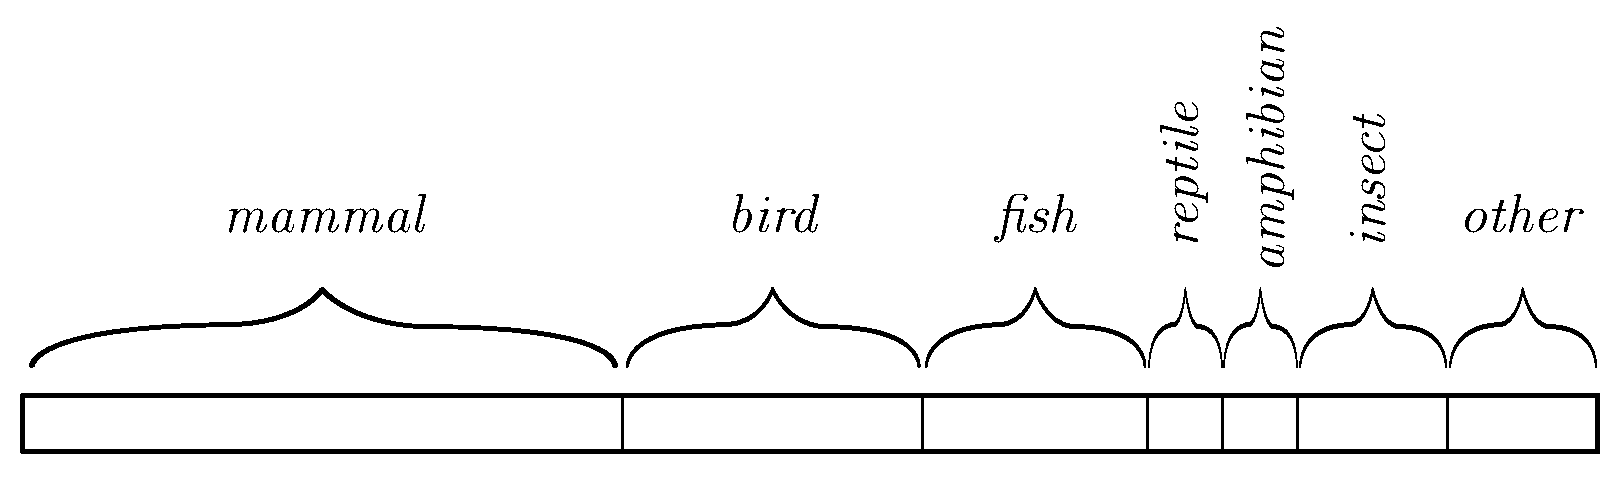
\includegraphics[scale = 0.3]{figs/baceCset.pdf}
\caption{\label{normalcset} Example of contrast set over the zoo data set. The extensional definitions are represented by the partition of the bar, the brackets are symbolizing their respective intensional definitions and their coverage, and finally their signs is written above them.}
\end{figure}

\begin{figure}[t]
\centering
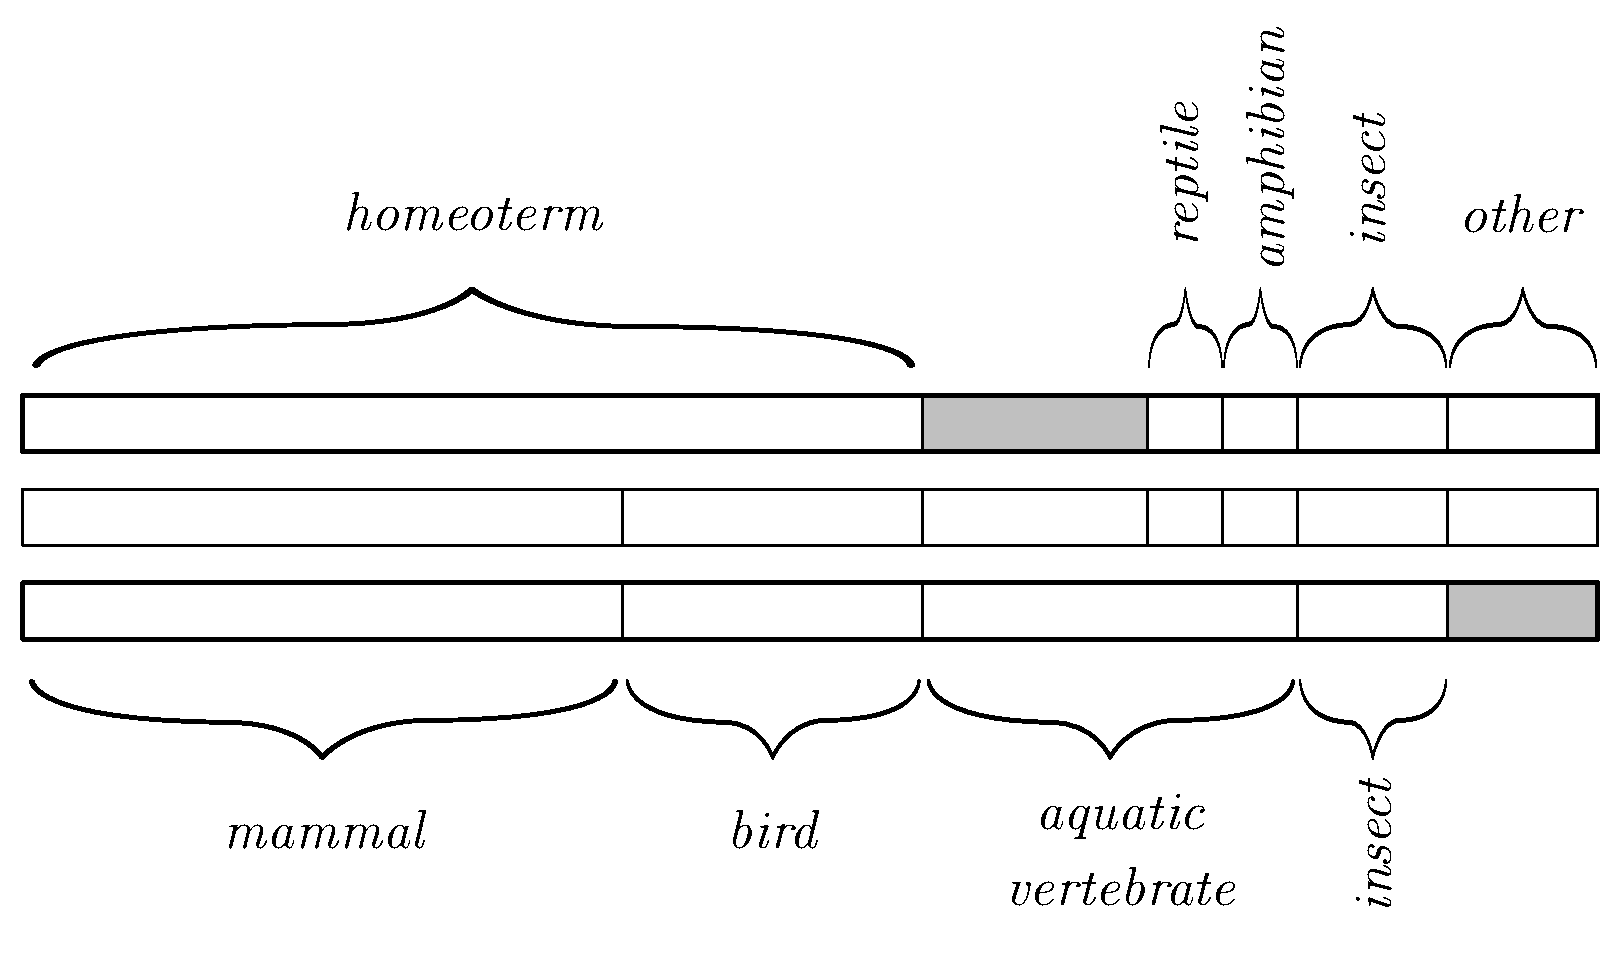
\includegraphics[scale = 0.3]{figs/exampleCsets.pdf}
\caption{\label{csetcomparison} Comparison of two contrast sets. The initial partition of the examples as found in the data set is represented between them. The gray part is representing missing examples from the overall context}.
\end{figure}

\section{Examples of First Order Disagreements}

\subsection{Data and Methodology}

The data set used for experiments on first order disagreements is the \emph{seat} data set, that has been created for the purpose of the present thesis. This data set is automatically generated by a procedural model, and consists of 150 entries divided into 3 categories of 50 instances each: \emph{chair}, \emph{armchair} and \emph{stool}. Each instance has a solution which is the name of a category, and a description. The description is a feature term $X_{i}$ with two main features: \emph{$X_{i}$.back-type} and \emph{$X_{i}$.arm-type}. The instances are generates such that:

\begin{itemize}
\item if the solution is \emph{armchair}, \emph{$X_{i}$.back-type $\doteq$ back} and \emph{$X_{i}$.arm-type $\doteq$ arms}
\item if the solution is \emph{chair}, \emph{$X_{i}$.back-type $\doteq$ back} and \emph{$X_{i}$.arm-type $\doteq$ no-arms}
\item if the solution is \emph{stool}, \emph{$X_{i}$.back-type $\doteq$ no-back} and \emph{$X_{i}$.arm-type $\doteq$ no-arms}
\end{itemize}

The rest of the features are filled with random values. Since they are not linked to the classification of the instances, these additional features should not appear in the generalizations of the agents and are just present as control features.

The data set \emph{seat} is used as a test data set $E_{test}$. Two additional data sets are created in order to be used as learning data sets, one for each agent. The first data set, $E_{t1}$, has 20 generated instances of chair, 20 generated instances of armchair and  10 generated instances of stool. However, the solution of the instances of stool are changed for \emph{chair} without modifying their descriptions. The second data set, $E_{t2}$, has 20 generated instances of chair, 20 generated instances of stool and  10 generated instances of armchair. Again, the solution of the instances of armchair are changed for \emph{chair}. These modifications, illustrated in figure \ref{}, lead to an overlap between the two sets of instances that have now \emph{chair} for solution.

Prior to the argumentation, two semiotic agents $A_{k}$ and $A_{-k}$ learn their initial contrast sets $A_{k}.K_{i}$ and $A_{-k}.K_{i}$ by using \textbf{ABUI} over respectively $E_{t1}$ and $E_{t2}$ as described in section \ref{}. This results in the situation shown in figure \ref{}, where the two concepts $C_{chair}^{k}$ and $C_{chair}^{-k}$ are in a relation of type overlap in the overall context. Since both agents have examples of instances from the three generated categories, this situation does not generate any second order disagreements: $A_{k}$ and $A_{-k}$ will always compute the two same local relations for a given pair of concepts. Once the agents have created their contrast set, they set their state to \emph{Initializing Argumentation}. Then, a token is randomly given to  one of the agent. The agents argue until their list of disagreement has become empty while they are in the \emph{Choosing a Disagreement} state.

\subsection{Exemplifying  Hypo/Hypernymy Disagreement}

In this exemplification, the classes \emph{chair} and \emph{armchair} are merged under the label \emph{chair} in the initial data set dealt to $A_{1}$. Therefore, we have $A_{1}$ that has an initial contrast set containing two concepts \emph{chair} and \emph{stool}, while $A_{2}$ has the standard initial contrast set containing \emph{chair}, \emph{armchair} and \emph{stool}. The initial setup guarantees that the concept \emph{chair} from $A_{2}$ is a hypernym of the concepts \emph{chair} and \emph{armchair} from $A_{2}$: $A_{1}$ learns that a seat is a chair if \emph{$X_{i}$.back-type $\doteq$ back} and a stool if \emph{$X_{i}$.back-type $\doteq$ no-back} and \emph{$X_{i}$.arm-type $\doteq$ no-arms} while $A_{2}$ retrieves correctly the generation rules of \emph{chair}, \emph{armchair} and \emph{stool} presented in the section above. Since the \emph{seat} data set does not pose any problem for inductive learning, the degree of error tolerated by the agents will only be $\tau_{E} = 1$ which is the smallest possible value.

In order to initiate the communication between the agent, the token is dealt to a random agent: let it be $A_{1}$. $A_{1}$ starts in the state 1, and send the intensional definitions $I(Chair^{1})$ and $I(Stool^{1})$ to $A_{2}$. Then $A_{1}$ passes the token to $A_{2}$, which also starts in the state 1, and $A_{2}$ sends the three intensional definitions $I(Armchair^{2})$, $I(Chair^{2})$ and $I(Stool^{2})$ to $A_{1}$. Then $A_{2}$ passes the token to $A_{1}$.

$A_{1}$ receives the token while being in the state 2. $A_{1}$ creates a hypothesis $H_{1}$ with the intensional definitions $I(Armchair^{2})$, $I(Chair^{2})$ and $I(Stool^{2})$ received from $A_{2}$ through the messages \emph{Assert}. Since the examples from the data set seat has been homogeneously distributed among the agents, $A_{1}$ evaluates correctly the relations $Chair^{1} \odot Armchair^{2}$, $Chair^{1} \odot Chair^{2}$ and $Stool^{1} \equiv Stool^{2}$ as its local relations. $A_{1}$ then sends all the r-triplets of its local relations through six messages:

\begin{multicols}{2}
\begin{enumerate}
    \item \emph{evaluation}($Chair^{1}, Armchair^{2}, (1,1,0)$)
    \item \emph{evaluation}($Chair^{1}, Chair^{2}, (1,1,0)$)
    \item \emph{evaluation}($Chair^{1}, Stool^{2}, (1,0,1)$)
    \item \emph{evaluation}($Stool^{1}, Armchair^{2}, (1,0,1)$)
    \item \emph{evaluation}($Stool^{1}, Chair^{2}, (1,0,1)$)
    \item \emph{evaluation}($Stool^{1}, Stool^{2}, (0,1,0)$)
\end{enumerate}
\end{multicols}

Then $A_{1}$ passes the token to $A_{2}$, which is now in state 2 and creates its own hypothesis $H_{2}$ with the intensional definitions $I(Armchair^{1})$ and $I(Chair^{1})$ received from $A_{1}$. As we mentioned in the paragraph above, the homogeneous distribution of the examples allow the agents to find the same relations between the concepts (the local relations are already the same as the overall relations), which means that $A_{2}$ sends the same evaluations to $A_{1}$:

\begin{multicols}{2}
\begin{enumerate}
    \item \emph{evaluation}($Armchair^{2}, Chair^{1}, (0,1,1)$)
    \item \emph{evaluation}($Armchair^{2}, Stool^{1}, (0,1,1)$)
    \item \emph{evaluation}($Chair^{2}, Chair^{1}, (1,0,1)$)
    \item \emph{evaluation}($Chair^{2}, Stool^{1}, (1,0,1)$)
    \item \emph{evaluation}($Stool^{2}, Chair^{1}, (1,0,1)$)
    \item \emph{evaluation}($Stool^{2}, Stool^{1}, (0,1,0)$)
\end{enumerate}
\end{multicols}

When $A_{1}$ receives the token from $A_{2}$, $A_{1}$ is in state 3. $A_{1}$ uses the local r-triplets that it computed in the precedent state along with the r-triplets that it received from $A_{2}$ through the \emph{evaluation} messages, and concludes that the overall relations are the same as its local relations. Therefore, $A_{1}$ does not send any example to $A_{2}$. Finally, $A_{1}$ creates a list $D_{1}$ with the observed disagreements. $A_{1}$ passes the token to $A_{2}$ that accomplishes its turn in state 3, compute the overall relations and draw the same conclusions as $A_{1}$, creates the list $D_{2}$ and passes back the token to $A_{1}$. At this point, after both agents have been thought the third state, the lists of disagreements are:

\begin{itemize}
    \item $D_{1} = [(Chair^{1}, Armchair^{2}, (1,1,0))$, $(Chair^{1}, Chair^{2}, (1,1,0))]$
    \item $D_{2}= [(Armchair^{2}, Chair^{1}, (0,1,1)), (Chair^{2}, Chair^{1}, (0,1,1))]$
\end{itemize}

$A_{1}$ receives the token. Since $A_{1}$ is now in the state 4 and has not received any message \emph{address} from $A_{2}$, $A_{1}$ chooses $Chair^{1}, Armchair^{2}, (1,1,0)$ as a random disagreement from $D_{1}$ and send a message \emph{address}($Chair^{1}, Armchair^{2}$) to $A_{2}$. Since $Chair^{1} \odot Armchair^{2}$, the next state of $A_{1}$ will be the state 5. $A_{1}$ passes the token to $A_{2}$, and $A_{2}$ receives the message \emph{address}($Chair^{1}, Armchair^{2}$). Since $Armchair^{2} \odot Chair^{1}$, the next state of $A_{2}$ will be the state 5.

At the beginning of its turn, $A_{1}$ creates the extensional definition of the concept $new_1$ that $A_{1}$ and $A_{2}$ will create to resolve the disagreement $Chair^{1}, Armchair^{2}, (1,1,0)$. This new concept will be the co-hyponym of $Chair^{1}$ with $Armchair^{2}$. Consequently, $A_{1}$ builds the set of positive examples $E^{1}_{+} = E(Chair^{1}) - E(Armchair^{2'})$ and the set of negative examples $E^{1}_{-} = E_{K1} - E^{1}_{+}$. Then, $A_{1}$ passes the token to $A_{2}$ which creates the sets $E^{2}_{+} = E(Chair^{1'}) - E(Armchair^{2})$ and $E^{2}_{-} = E_{K2} - E^{2}_{+}$. Due to the experimental setup of this example, each set $E^{x}_{+}$ will contain the examples with the features \emph{$X_{i}$.back-type $\doteq$ back} and \emph{$X_{i}$.arm-type $\doteq$ no-arms} of the context $E_{Kx}$.

The agents $A_{1}$ and $A_{2}$ will now enter in a loop from which they will exit only once they have each found an intensional definition, $I^{1}_{+}$ and $I^{2}_{2}$, that can be the intensional definition of  \emph{both} $E^{1}_{+}$ and $E^{2}_{+}$. When $A_{1}$ starts in state 6, it creates an intensional definition $I^{1}_{+}$ and sends it to $A_{2}$ with a message \emph{Assert}($new_1$, $I^{1}_{+}$). After receiving the token, $A_{2}$ creates its intensional definition  $I^{2}_{+}$ and sends a message \emph{Assert}($new_1$, $I^{2}_{+}$) to $A_{1}$. Additionally, $A_{2}$ evaluates the intensional definition $I^{1}_{+}$ that it received. Since $I^{1}_{+}$ subsumes all the examples from $E^{2}_{+}$ without subsuming any examples from $E^{2}_{-}$, $A_{2}$ also send a message \emph{accept}($new_1$, $I^{1}_{+}$) to $A_{1}$. When $A_{1}$ receives the token, $A_{1}$ acknowledges that $A_{2}$ agreed upon the intensional definition $I^{1}_{+}$ through a message \emph{agree}. Then, $A_{1}$ evaluates the intensional definition $I^{2}_{+}$ that it received and notices that $I^{2}_{+}$ subsumes all the examples from $E^{1}_{+}$ without subsuming any example from $E^{1}_{-}$. Therefore, $A_{1}$ sends a message \emph{agree}($new_1, I^{2}_{+}$) to $A_{2}$. Now that $A_{1}$ has agreed upon the intensional definition of $A_{2}$ and knows that $A_{2}$ agreed upon its intensional definition, $A_{1}$ is ready to move to the state 7. When $A_{2}$ gets the token, it is notified by $A_{1}$ that $I^{2}_{+}$ has been agreen upon. $A_{2}$ is now also ready to move to the state 7.

At the end of the state 6, both agents have found in parallel a similar intensional definition:

\begin{itemize}
    \item $I^{1}_{+}$ = \emph{$X_{i}$.back-type $\doteq$ back} and \emph{$X_{i}$.arm-type $\doteq$ no-arms}
    \item $I^{2}_{+}$ = \emph{$X_{i}$.back-type $\doteq$ back} and \emph{$X_{i}$.arm-type $\doteq$ no-arms}
\end{itemize}

$A_{1}$ is now in state 7 and creates a new concept $new_1^{1}$. Since the current disagreement ($Chair^{1}$, $Armchair^{2}$, $(1,1,0)$) is a hypo/hypernymy disagreement, and since $Armchair^{2}$ belongs to $A_{2}$'s contrast set, $A_{1}$ also create a concept $new_2^{1}$ and remove $Armchair^{2'}$ from $H_{1}$. When $A_{2}$ gets the token, it creates the concept $new_1^{2}$. Since $Armchair^{2}$ belongs to $K_{2}$, $A_{2}$ removes $Armchair^{2}$ from $K_{2}$ and creates a new concept $new_2^{2}$. The composition of the new concepts are the following:

\begin{itemize}
    \item $new_1^{1} = (new_1, I^{1}_{+}, E^{1}_{+})$
    \item $new_2^{1} = (new_2, I(Armchair^{2}), E(Armchair^{2'}))$
    \item $new_1^{2} = (new_1, I^{2}_{+}, E^{2}_{+})$
    \item $new_2^{2} = (new_2, I(Armchair^{2}), E(Armchair^{2}))$
\end{itemize}

Since the current disagreement is a hypo/hypernymy disagreement, the next state of $A_{1}$ and $A_{2}$ is the state 8. $A_{1}$ deletes the hypernym $Chair^{1}$ from $K_{1}$, then passes the token to $A_{2}$ that deletes $Chair^{1'}$ from $H_{2}$. Moving to the state 9, $A_{1}$ evaluates the relations between $new_1^{1}$, $new_2{1}$ and the concepts from $K_{2}$ and sends them to $A_{2}$ through \emph{evaluation} messages:

\begin{multicols}{2}
\begin{enumerate}
    \item \emph{evaluation}($new_1^{1}, Chair^{2}, (0,1,0)$)
    \item \emph{evaluation}($new_1^{1}, Stool^{2}, (1,0,1)$)
    \item \emph{evaluation}($new_2^{1}, Chair^{2}, (1,0,1)$)
    \item \emph{evaluation}($new_2^{1}, Stool^{2}, (1,0,1)$)
\end{enumerate}
\end{multicols}

Then $A_{1}$ passes the token to $A_{2}$ which does the same and sends to $A_{1}$:

\begin{multicols}{2}
\begin{enumerate}
    \item \emph{evaluation}($new_1^{2}, Stool^{1}, (1,0,1)$)
    \item \emph{evaluation}($new_2^{2}, Stool^{1}, (1,0,1)$)
\end{enumerate}
\end{multicols}

$A_{1}$ receives the token and goes through the state 10, where $A_{1}$ computes the overall relations between the new concepts and the old ones by adding $new_1^{1}$ and $new_2^{1}$ to both $K_{1}$ and $H_{1}$. Then, $A_{1}$ observes that $new_1^{1} \equiv Chair^{2}$ and deletes $Chair^{2}$ from $H_{1}$. $A_{1}$ finishes its turn by updating the list of disagreement $D_{1}$, that becomes empty.

When $A_{2}$ receives the token, it computes the overall relations and add $new_1^{2}$ and $new_2^{2}$ to both $K_{2}$ and $H_{2}$. Since $new_1^{1} \equiv Chair^{2}$, $A_{2}$ deletes $Chair^{2}$ from $K_{2}$. $A_{2}$ finishes its turn by updating the list of disagreement $D_{2}$, that also becomes empty.

Going back to state 4, $A_{1}$ finds $D_{1}$ empty, which means that its next state will be the state 12. When $A_{2}$ receives the token, it finds $D_{2}$ empty: its next state will also be 12.



\section{Examples of Second Order Disagreements}

The following section will present four examples of argumentation in the situation where semiotic agents have to face second order disagreements, corresponding to the four cases of second order disagreement highlighted in the figure \ref{}. The examples will use the data set \emph{zoology}, which is more diverse than \emph{seat} with seven classes. However, the ontological structure of \emph{zoology} is more simple than \emph{seat} with a depth of one, making it similar to description logic as the examples are represented as vectors of features' values.

This data set is perfect to test the argumentation involving second order disagreements. On the contrary to the section \ref{} where each agent had distinct contexts, the experiments on second order disagreements involve two agents sharing almost all of the examples from their context. The only examples that are present in only one context are selected to cause the second order disagreements, enabling one agent to see a relation between to concepts with more accuracy than an other. 

\subsection{Data and Methodology}

% Presentation of the Zoology Data Set
The data set used for experiments on second order disagreements is the \emph{zoology} data set from the UCI Machine Learning Repository\footnote{http://archive.ics.uci.edu/ml/datasets/zoo}.
%% Presentation of the different categories
The data set contains animal species as instances, clustered into seven distinct categories. The label of these categories will be listed, followed by their corresponding number of instances between parentheses: \emph{mammal}(41), \emph{bird}(20), \emph{reptile}(5), \emph{fish}(13), \emph{amphibian}(4), \emph{insect}(8) and \emph{other}(10). There is a total of 101 instances in the data set. During the rest of the section, regarding the notation $C_{i}^{k}$, the following abbreviations will be used instead of the full sign \emph{i}: \emph{mammal} = \emph{mam}, \emph{reptile} = \emph{rep}, \emph{amphibian} = \emph{amph} and \emph{insect} = \emph{ins}.
%% Presentation of the different attributes (features)
Each instance has a \emph{sort} (see $\psi$-term formalism) with two main features: a solution (the label of the instance's category) and a description. The description is an array of 17 attributes that can have either a boolean or a numeric value: for instance, the number of legs of the specie or 0 and 1 if the feature is boolean, such as \emph{lactation}.

\subsubsection{Setting Up Contrast Sets for the Examples}

% Creating the contrast sets
Contrast sets learned over the same data sets are remarkably consistent: two contrast sets created over the same data set are usually in synchronic agreement even with a value of $t = 1$. This is at least the case for simple contrast sets like \emph{seat} and \emph{zoology}. In order to prove this, we have evaluated the measures $m_{1}$, $m_{2}$ and $m_{3}$ over 100 creations of contrast sets $A_{k}.K$ and $A_{-k}.K$ using \emph{zoology}. In all the hundred of trials, $A_{k}.K$ and $A_{-k}.K$ were always satisfying contrast sets without any synchronic disagreements ($m_{1}$, $m_{2}$ and $m_{3}$ = 0). Measuring $m_{4}$ to evaluate the diachronic agreement was meaningless since no argumentation held place, thus $A_{k}.K = A_{k}.K_{i}$. Consequently to the absence of disagreement between two agents having this version of the contrast set, any arising disagreement in our scenario can only be caused by the experimental setup that we will introduce.

There are two possible modifications of the contrast sets that can provoke a situation of synchronic disagreement. The first modification consists in changing the label of some instances in the data set, as instances of stools and armchairs have been relabeled as \emph{chair} in the section \ref{}. However, it is impossible to create second order disagreements with such modifications as it does not alter the examples of the contrast sets' context. The only way to create second order disagreement is by deleting some instances from the data set, in order to introduce differences between the contrast sets' context.

\subsubsection{Setting Up the First Case of Second Order Disagreement}

The first case of second order disagreement is due to an overall relation of type overlap. In order to create this overlap, we changing the labels \emph{mammal} and \emph{fish} to $s_{1}$ in $E_{l1}$ and the labels of \emph{fish} and \emph{bird} to $s_{2}$ in $E_{l2}$. This way, the relation $ov.r(C_{1}^{1}, C_{2}^{2})$ is of type overlap. At this point, the local relations $r(C_{1}^{1},C_{2}^{1},A_{1}.E_{K})$ and $r(C_{2}^{2},C_{1}^{2},A_{2}.E_{K})$ will also be of type overlap since they can partition the overall context.

In the first case of second order disagreement, $A_{1}$'s local relation is of type equivalence, which means that $E_{1}^{1}$ and $E_{2}^{1}$ should contain the same examples. For this reason, once the contrast set has been learned, we delete the examples of $E_{mam}$ and $E_{bird}$ from $A_{1}.E_{K}$, leaving only the examples of $E_{fish}$ to be subsumed by both $I_{1}^{1}$ and $I_{2}^{1}$. $A_{1}$ now sees its local relation $r(C_{1}^{1},C_{2}^{1},A_{1}.E_{K})$ as of the equivalence type. Since $I_{mam}^{1}$ is not covering any example anymore, $C_{mam}^{1}$ is deleted from $A_{1}.K$.

In the first case of second order disagreement, $A_{2}$'s local relation is of disjunction type, which means that $E_{1}^{2}$ and $E_{2}^{2}$ should not have any example in common. For this reason, once the contrast set has been learning, we delete the examples of $E_{fish}$ from $A_{2}.E_{K}$, leaving no example to be subsumed by both $I_{1}^{2}$ and $I_{2}^{2}$. $A_{2}$ now sees its local relation $r(C_{2}^{2},C_{1}^{2},A_{2}.E_{K})$ as of the disjunction type.

\subsubsection{Setting Up the Second Case of Second Order Disagreement}

This is similar to first case of second order disagreement, but EXPLAIN HERE DIFFERENCE the second case of second order disagreement is due to an overall relation of type overlap. In order to create this overlap, we proceed as in section \ref{} by changing the labels \emph{mammal} and \emph{fish} to $s_{1}$ in $E_{l1}$ and the labels of \emph{fish} and \emph{bird} to $s_{2}$ in $E_{l2}$. The relation $ov.r(C_{1}^{1}, C_{2}^{2})$ and the local relations $r(C_{1}^{1},C_{2}^{1},A_{1}.E_{K})$ and $r(C_{2}^{2},C_{1}^{2},A_{2}.E_{K})$ are of type overlap again.

In the second case of second order disagreement, $A_{1}'s$ local relation is of type inclusion. One of the sets $E_{1}^{1}$ and $E_{2}^{1}$ should be a subset of the other. For this reason, once the contrast set has been learned, we delete the examples of $E_{mam}$ from $A_{1}.E_{K}$, leaving only the examples of $E_{fish}$ to be subsumed by $I_{1}^{1}$ but both the examples of $E_{fish}$ and $E_{bird}$ to be subsumed by $I_{2}^{1}$. $A_{1}$ now sees its local relation $r(C_{1}^{1},C_{2}^{1},A_{1}.E_{K})$ as of the inclusion type, with $h(C_{1}^{1},C_{2}^{1}, \subset)$.

Similarly to the first case of second order disagreement, in the second case of second order disagreement $A_{2}$'s local relation is of type disjunction. For this reason, we proceed as in the first case of second order disagreement and once the contrast set has been learning, we delete the examples of $E_{fish}$ from $A_{2}.E_{K}$, leaving no example to be subsumed by both $I_{1}^{2}$ and $I_{2}^{2}$. $A_{2}$ now sees its local relation $r(C_{2}^{2},C_{1}^{2},A_{2}.E_{K})$ as of the disjunction type.
 
\subsubsection{Setting Up the Third Case of Second Order Disagreement}

The third case of second order disagreement is due to an overall relation of type inclusion. In order to create this inclusion, we change the label \emph{mammal} to $s_{1}$ in $E_{L1}$ and the labels  \emph{mammal} and \emph{fish} to $s_{2}$ in $E_{l2}$. The relation $ov.r(C_{1}^{1}, C_{2}^{2})$ and the local relations $r(C_{1}^{1},C_{2}^{1},A_{1}.E_{K})$ and $A_{2}$ are of type inclusion, with $h(C_{1}^{1},C_{2}^{1}, \subset)$.

In the third case of second order disagreement, $A_{1}'s$ local relation is of type equivalence, which means that $E_{1}^{1}$ and $E_{2}^{1}$ should contain the same examples. For this reason, once the contrast set has been learned, we delete the examples from  $E_{fish}$ from $A_{1}.K$. This leaves only the examples from $E_{mam}$ to be subsumed by both $I_{1}^{1}$ and $I_{2}^{1}$. $A_{1}$ now sees its local relation $r(C_{1}^{1},C_{2}^{1},A_{1}.E_{K})$ as of the equivalence type. Since $I_{fish}^{1}$ is not covering any example anymore, $C_{fish}^{1}$ is deleted from $A_{1}.K$.

There is no need to change anything from $A_{2}$'s contrast set, since $A_{2}$ already sees its local relation $r(C_{2}^{2},C_{1}^{2},A_{2}.E_{K})$ as of the inclusion type.

\subsubsection{Setting Up the Fourth Case of Second Order Disagreement}

The fourth case of second order disagreement is due to an overall relation of type overlap but is better described as consisting of 
 three sub-cases $c_{1}$, $c_{2}$ and $c_{3}$. In order to create this overlap, we proceed as for setting up the first and second cases of second order disagreement: by changing the labels \emph{mammal} and \emph{fish} to $s_{1}$ in $E_{l1}$ and the labels of \emph{fish} and \emph{bird} to $s_{2}$ in $E_{l2}$. The relation $ov.r(C_{1}^{1}, C_{2}^{2})$ and the local relations $r(C_{1}^{1},C_{2}^{1},A_{1}.E_{K})$ and $r(C_{2}^{2},C_{1}^{2},A_{2}.E_{K})$ are of type overlap.

The particularity of all the cases regrouped as the fourth case of second order disagreement is that $A_{2}$'s local relation $r(C_{2}^{2},C_{1}^{2},A_{2}.E_{K})$ is of type overlap, which means that we do not change anything to $A_{2}$'s contrast set.

However, the local relations of $A_{1}$ in $c_{1}$, $c_{2}$ and $c_{3}$ are respectively of type equivalence, inclusion and disjunction (see figure \ref{fig:VennCases}). For this reason, in $c_{1}$ we will modify the contrast set $A_{1}.K$ as in the set up of the first case of second order disagreement. We delete the examples of $E_{mam}$ and $E_{bird}$ from $A_{1}.E_{K}$ such that $A_{1}$ now sees its local relation $r(C_{1}^{1},C_{2}^{1},A_{1}.E_{K})$ as of the equivalence type.

In $c_{3}$, $A_{1}.K$ is modified as in the set up of the second case of second order disagreement by deleting the examples of $E_{mam}$ from $A_{1}.E_{K}$ such that $A_{1}$ now sees its local relation $r(C_{1}^{1},C_{2}^{1},A_{1}.E_{K})$ as of the disjunction type.

Finally, in $c_{2}$, the examples from $E_{mam}$ are removed from $A_{1}.E_{K}$, leaving only the examples of $E_{fish}$ to be subsumed by $I_{1}^{1}$ but both the examples of $E_{fish}$ and $E_{bird}$ to be subsumed by $I_{2}^{1}$. This causes $A_{1}$ to see its local relation $r(C_{1}^{1},C_{2}^{1},A_{1}.E_{K})$ as of the inclusion type, with $h(C_{1}^{1},C_{2}^{1}, \subset)$.

\section{Evaluation of the Systematic Approach}

\section{Evaluation of the Lazy Approach}

\chapter{Evaluations}\label{Evaluations}
%%% Presentation
\section{Presentation of the Experiments}

%% Subsection Parameters
\subsection{Parameters}
Before introducing the variables (dependent and independent) of our experiments, we will discuss its parameters. The parameters are not tested individually for each scenario, instead they are pre-selected. There are three parameters in our model:

\begin{enumerate}
    \item the error threshold $\tau_{E}$
    \item the argument acceptability $aa$ of the ABUI algorithm that generates the generalizations
    \item the redundancy $r$ between the two initial contexts of the agents.
\end{enumerate}

\paragraph{Error threshold:} the error threshold is the parameter $\tau_{E}$ already presented in Section \ref{sec:DegOfErr}. Referred as ``the degree of error tolerated'' in the figures, it gives the number of examples that is required by the agents for overall pairing partial sets to be taken into account in the definition of overall pairing relations. A different error threshold is linked to every data set, as the value of the error threshold affects the number of classes available to set up disagreements.

\paragraph{Argument Acceptability:} the argument acceptability is a parameter of the ABUI algorithm that determines weather or not a generalization generated by ABUI is considered satisfying with regard to the constraints that the model was extensionally requiring of it. For instance, during the construction of a counter-argument $\alpha$, an agent builds a set of positive and negative examples that $\alpha$ should and should not cover. In this situation, the argument acceptability is the accuracy of $\alpha$ over the sets of positive and negative examples above which the ABUI algorithm considers that $\alpha$ is satisfying enough to endorse the role of a counter-argument. By default, the argument acceptability is 0.75 in our experiments, as it is the default value used in the AMAIL argumentation framework.

\paragraph{Redundancy:} the redundancy is the percentage of each agent's initial context that is shared among them. If the agents receive 60 labeled examples at the beginning of the experiment, 30 of which are in both initial context, the redundancy is $50 \%$. If the same 60 examples are the initial contexts of both agents, the redundancy is $100 \%$. The redundancy is defined by the ratio of shared examples, the label of these examples are not taken into account and two agents might have $r=100 \%$ although they do not share a single right-path association. By default, the redundancy is zero in our experiments, as it is the most complex scenario four our agents to reach mutual intelligibility over. Indeed, a redundancy of 0 indicates that no information is initially shared by the agents in the form of examples.

%% Subsection
\subsection{Variables}
\label{sec:variables}

This section presents the variables that will be found in our experiments. They are presented in two distinct categories: independent variables (IV) and dependent variables (DV).
% IV
We have four independent variables: \emph{domain}, \emph{strategy}, \emph{setup disagreements} and \emph{number of initial concepts}.
% DV
There is a total of four dependent variables: the \emph{Synchronic Agreement Ratio}(SAR), the \emph{Diachronic Agreement Ratio}(DAR), the \emph{Exchanged Examples Ratio}(EER), the \emph{Number of Expected Concepts}(NEC) and the \emph{Number of Final Concepts} (NFC).

% VI
\subsubsection{Independent Variables (IV)}

\paragraph{Domain}
% The already presented data-sets
Each domain corresponds to a different data-set. The first two domains correspond to two of the three data-sets already presented in Chapter \ref{Examples}: \emph{Zoology} and \emph{Sponges}.
% We add Soybean minus the four small classes
The remaining domain \emph{Soybean} correspond to the eponymous data-set. The Soybean data-set has 307 instances of soybean observations spread among 19 classes of soybean diseases. There are 35 categorical attributes, some nominal and some ordered.
% Domains come with a set of parameters
While the experiments always use a redundancy of $0\%$ and an argument acceptability of $0.75$, each domain has its associated error threshold.


\paragraph{Strategy}
% The two strategies
Our model is divided in two strategies: the systematic and the lazy.
% Systematic
The systematic strategy is presented in Chapter \ref{SystematicStrategy} and is a strategy that focuses on preventing any disagreement that could occur on the overall context of the two agents.
% Lazy
The lazy strategy is presented in Chapter \ref{LazyStrategy} and unlike the systematic strategy, it focuses on solving disagreements on connected sets of disagreements once the agents encounter an error in their naming game.

\paragraph{Setup Disagreements (SDC)}
While the actual number of disagreements that the two agents will encounter depends on the learning of their initial contrast sets, the disagreements that we expect the agents to solve are experimentally set up. The set up of these disagreements has already been discussed in Chapter \ref{Examples}. This set up takes two parameters: the type of disagreements (overlap, hypo/hypernymy, synonymy or homonymy) that are set up, and for each type, the number of these disagreements.

\paragraph{Number of Initial Concepts (OCC)}
The number of initial concepts is the number of categories that are present in the data-set related to the experiment's domain. For the lowest possible error threshold, one, we have 3 concepts in the \emph{Sponges} domain, 7 concepts in the \emph{Zoology} domain, and 19 concepts in the \emph{Soybean} domain. However, increasing the error threshold $\tau_{E}$ decreases the number of initial concepts that can be used, as the initial concepts should contain at least $\tau_{E}$ examples.

% VD
\subsubsection{Dependent Variables (DV)}

\paragraph{Count of Disagreements(C:type,context)} The first measure of an experiment success is the count of each type of disagreements that exist between the two agent at the beginning and at the end of an argumentation. We therefore have an initial and a final count of disagreements, for each type of disagreements: self-disagreements, overlap disagreements, hypo/hypernymy disagreements, synonymy disagreements, homonymy disagreements, indistinguishable disagreements and untranslatable disagreements. Since there is a distinction between the local and the overall disagreements, the count can be local (as one agent sees it) or overall (as the experimenter sees it). Our model stops when there is no overall disagreement detected by the agents anymore, and by extension no local disagreement either. For this reason, we always expect the final count, either local or global and for each type of disagreement, to be equal to zero. Other variables will give a more nuanced measure of our model success.

\paragraph{Synchronic Agreement Ratio (SAR)} The Synchronic Agreement Ration, or SAR, is the ratio between the of examples from the overall context that are named through a left path association with the same unique sign by both agents when presented to them, over the total number of examples in the overall context. The SAR measures how well the agents have reached mutual intelligibility. %The RSA is defined in Definition \ref{def:SAR}.

\begin{restatable}[SAR]{df}{SAR}
\label{def:SAR}
Let $A_{1}$ and $A_{2}$ be two agents, and $K1$ and $K2$ be their contrast sets. The Synchronic Agreement Ratio of the two agents is:

\[
SAR(A_{1},A_{2}) = \frac{|\{ e \in U_{O} | e \prescript{l}{K1}{\mapsto} s \wedge  e \prescript{l}{K2}{\mapsto} s \}|}{|U_{O}|} 
\]

\end{restatable}

\paragraph{Diachronic Agreement Ratio (DAR)} The Diachronic Agreement Ratio in an agent is the additive inverse of the ratio between (1) the number of pairs of examples from an agent's initial context that were in two different concepts in the initial contrast set that later are in the same concept in the final contrast set, and (2) the number of pairs of examples that were in two different concepts in the initial contrast set. The DAR is a measure of refinement that shows how well the monotonic evolution of the contrast sets have been respected through the argumentation. % The DAR is defined in Definition \ref{def:DAR}:

\begin{restatable}[DAR]{df}{DAR}
\label{def:DAR}
Let $A$ be an agent that has $K = (U,Q)$ for initial contrast set and $K' = (U',Q')$ for final contrast set. The Diachronic Agreement Ratio of $A$ is:

\[
DAR(A) = 1 - \frac{| \{e_{1},e_{2} \in U | e_{1} \prescript{l}{K}{\mapsto} s \wedge e_{2} \prescript{l}{K}{\mapsto} s  \wedge e_{1} \prescript{l}{K'}{\mapsto} s \wedge e_{2} \prescript{l}{K'}{\mapsto} s' \wedge s \neq s' \} |}{| \{e_{1},e_{2} \in U | e_{1} \prescript{l}{K'}{\mapsto} s \wedge e_{2} \prescript{l}{K'}{\mapsto} s' \wedge s \neq s' \} |}
\]

\end{restatable}

\paragraph{Exchanged Examples Ratios (EER)} The exchanged examples ratio (EER) corresponds to the number of examples that have been sent from one agent to the other through messages, divided by the number of examples in the overall context.

\paragraph{Coverage Ratio (CR)} The coverage ratio (CR) corresponds to the number of examples from the overall context that can be associated with a sign by an agent through left-path associations, divided by the number of examples in the overall context.

\paragraph{Observed Disagreements Count (ODC)} Unlike the set-up disagreements (SD), the observed disagreements (OD) are disagreements \emph{stricto-sensus}. They are the disagreements that are observed between the agents after they learned their initial contrast sets. Similarly to the set-up disagreements, we measure their types and number. The setup disagreements are unlikely to be the only disagreements found between our two agents once they learn they initial contrast sets, as they built their knowledge upon partial information on the overall context. ODs can be counted before or after the argumentation, and using either the local context of one agent or the overall context.

\paragraph{Final Disagreements Count (FDC)} The final disagreements are the disagreements found at the end of the argumentation. While their count is interesting, a number of final disagreement equals to zero is synonymous of full synchronic agreement between the agents only in scenarios where we are not accounting a degree of error. When accounting a degree of error, there can be no disagreement between the agents while the agents still associate some examples with different signs (in a proportion indexed on the error threshold that is therefore fixed).

\paragraph{Number of Expected Concepts (NEC)} The number of expected concepts represents the total number of concepts that should be expected in a contrast set that has a concept for each polylexematic class in the combined left-path associations of both agents -- which corresponds to the result of a brute force approach to the problem addressed in this thesis. Given two agents $A_{1}$ and $A_{2}$ that have respectively $m$ and $n$ concepts in their contrast sets, their maximum number of expected concept is $2^{m+n} - 1$ concepts, which corresponds to the number of possible combinations between the agents' adjunct sets minus the empty set.

\paragraph{Number of Final Concepts (NFC)} The number of final concepts, or NFC, is the number of concepts in the final contrast set of one agent. For an agent $A$ with a final contrast set $K = (U,Q)$, the NFC is equal to $|Q|$. The NFC can be measured in any of the two agents, as our protocol ensures that both agents end the argumentation with the same number of concepts in their contrast sets.

%% Elements tested
\subsection{Tested Properties}

Our model is evaluated through an array of hypotheses that are tested. There is a total of seven tested hypotheses, each one corresponding to different combinations of experiments and testing a specific trait of our model.

\begin{enumerate}
    \item \textbf{H1: Generality} Our model allows two agents to reach mutual intelligibility without creating diachronic disagreements regardless of the type or combinations of types of disagreements between these two agents.
    \item \textbf{H2: Domain Independence}: Our model allows two agents to reach mutual intelligibility without creating diachronic disagreements regardless of the domain of their overall context.
    \item \textbf{H3: Coverage Preservation} Our model allows two agents to reach mutual intelligibility without restraining the context of the agents, as the overall context of the agents should not lose examples through the argumentation.
    \item \textbf{H4: Efficiency} Our model allows two agents to reach mutual intelligibility without exchanging any significant portion of their contexts.
    \item \textbf{H5: Scalability} A linear increase of size of the overall context does not exponentially increase the number of generalizations that need to be exchanged in order for the agent to reach mutual intelligibility.
    \item \textbf{H6: Simplicity} The number of concepts in each contrast-set after that the agents have reached mutual intelligibility is the number of expected concepts NEC that can be computed before the argumentation.
    \item \textbf{H7: Paradigm Shift} The SAR and the DAR achieved by an AMAIL argumentation after an argumentation using our model is better than the SAR and DAR achieved by an AMAIL argumentation alone, while the total computation time of our model plus an AMAIL run is lesser than an AMAIL run alone.
\end{enumerate}

%%% GENERALITY
\section{Generality}

%% We test generality on different tasks over the same domain (soybean)
The hypothesis of generality postulates that both approaches of our model can resolve each possible combination of disagreements between two agents' contrast sets, increasing their SAR while keeping their perspective DAR at one. In order to test this hypothesis, we used the Soybean data set to setup variable disagreements between two agents. We counted the number of disagreements before and after argumentation, along with the SAR and the DAR. In order to evaluate this hypothesis on a great number of disagreements and combinations of disagreements, we have repeated this experiment 200 times.

% Order the types
Four types of disagreements are being setup in each experiment: overlap, hypo/hypernymies, synonymies and homonymies. These four types are randomly ordered for each experiment, and a random number of each disagreement type is selected and then setup, one type after the other. For instance, if the overlap type has been ordered first, we select a random number between 0 and the number of classes of Soybean with more than $\tau_{E}$ examples divided by three (the number of classes required to setup an overlap disagreement) and we merge as many time three random classes in order to obtain as many overlap disagreements. For each of the 200 runs of the experiment, we setup a new random arrangement of disagreements.

% The VI are the disagreements that we set up
The independent variables of this experiment are the types of disagreements that have been setup and their number (SDC). The experiment is always using the Soybean data set, an error threshold of $\tau_{E} = 5$ and an argument acceptability of $0.75$.
% The VD are the MSA, the MDA, the SC and the EEC
The main dependent variables are the SAR and the DAR, in order to measure to which extend our model reached a mutual intelligibility in a monotonic way. These variables are completed by the different example counts (ODC, FDC) and the coverage ratio (CR).

The setup disagreements are unlikely to be the only disagreements found between our two agents once they learn they initial contrast sets, as they built their knowledge upon partial information on the overall context. For this reason, we also count the number of observed disagreements. The number of observed disagreements can be counted before or after the argumentation, and using either the local context of one agent or the overall context. The number of observed disagreements is an additional dependent variable.

\subsection{Systematic Strategy}

The results of this experiment are shown in Figures \ref{fig:gen_count}, \ref{fig:gen_intro} and \ref{fig:gen_local} below. Figure \ref{fig:gen_count} displays the count of disagreements in our experiment. The left figure represents the global counts, while the right picture separates the counts for each different type of disagreement. The counts are done at three different moments of the argumentation: the set up disagreements are counted \emph{before} the argumentation, as they are the arguments that we set up in the agents learning data sets prior to the construction of their initial contrast sets. The observed disagreements are counted \emph{at the beginning} of the argumentation, once the initial contrast sets have been learned. The final disagreements are counted \emph{after} the argumentation, and should therefore always be equal to 0.

\begin{figure}
    \centering
    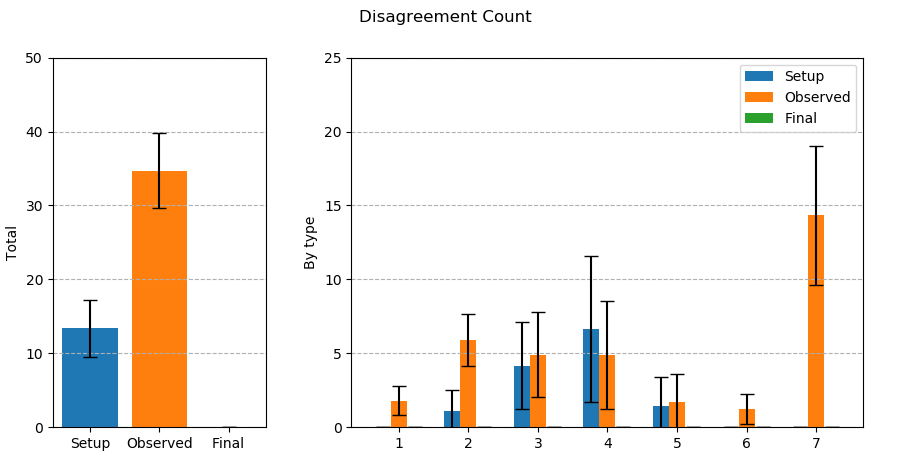
\includegraphics[width=\textwidth]{results/Figure_3_resized.png}
    \caption{The left plot presents the total count of disagreements, for all their types. On the right plot, the y-axis shows the  disagreement count for the types of disagreement displayed in the x-axis: 1.Self-Disagreement, 2.Overlap, 3. Hypo/hypernym, 4. Synonym, 5.Homonym, 6.Indistinguishable disagreement, 7.Untranslatable disagreement.}
    \label{fig:gen_count}
\end{figure}

In the left part of Figure \ref{fig:gen_count}, we can observe that the number of observed disagreements is more than twice the number of disagreements that have been set up. While disagreements spontaneously arise between two agents once they learned their first contrast sets over two different contexts, setting up disagreements increases the heterogeneity between the two agents' representations and causes a higher number of disagreements. The set up disagreements can be seen as ``stems'' for the observed disagreements. The final number of disagreements, which is counted after each argumentation, is always zero. This is not surprising, as an absence of disagreement is not necessarily equivalent to a full mutual agreement if the model admits a positive error threshold. The absence of overall disagreements is in fact the condition that tests the end of the argumentation between the agents in the systematic strategy, and therefore an equal-to-zero number of disagreements after the argumentation was expected.

The right part of Figure \ref{fig:gen_count} breaks down the count of disagreements for each different types of disagreements. As mentioned before, the only set up disagreement types that have a positive count are following: overlap,  hypo/hypernym,  synonym and the homonym. The distribution of the set up disagreements is directed by the cost of setting up each type: for instance, setting up an overlap requires three classes from the initial data set. On the other hand, setting up a synonymy only requires one class. Moreover, certain disagreements are causing other type of disagreements: for instance, setting up an overlap also sets up two hypo/hypernym disagreements.

The distribution of the observed disagreements is very different from the distribution of the setup disagreements. For instance, the most observed type of disagreement from the four types that are setup is the overlap disagreement, which was also the least set up type of disagreement. Indeed, since setting up an overlap requires to use 3 classes versus two at most for the other three types, they are expected to be less. The high incidence of overlap disagreements in the observed disagreements is an indicator that the overlap disagreement is the most likely to appear spontaneously when two agents learn their concepts over different contexts. Moreover, we can see that the most observed type of disagreements is the untranslatable disagreement. Since our error threshold is low ($\tau_{E} = 5)$, and since the Soybean data set has many small classes having about this number of examples, this is due to the agents over-fitting their intensional definitions because of the scarcity of examples in their initial data sets.


\begin{figure}
        \centering
        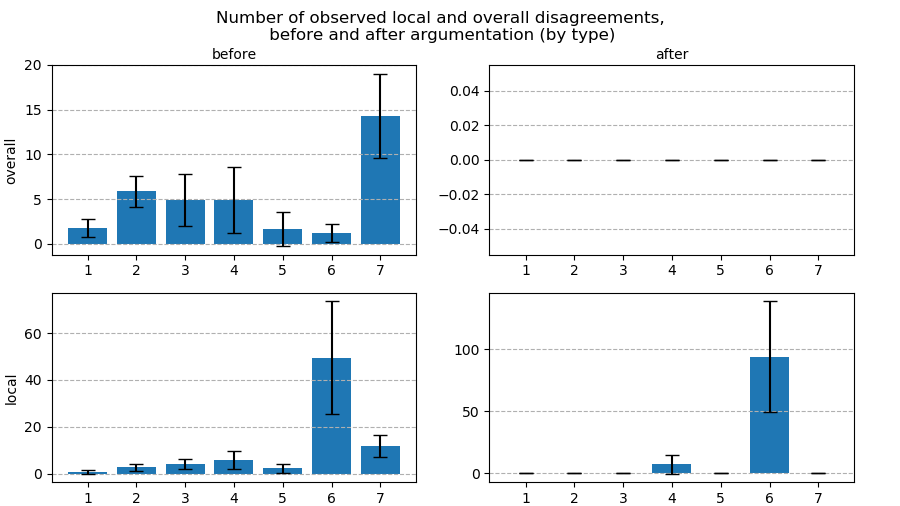
\includegraphics[width=\textwidth]{results/Figure_2_resized.png}
        \caption{The y-axis displays the count of each of the types of disagreement displayed in the x-axis: 1.Self-Disagreements, 2.Overlaps, 3. Hypo/hypernymies, 4. Synonymies, 5.Homonymies, 6.Indistinguishable disagreements, 7.Untranslatable disagreements}
        \label{fig:gen_local}
\end{figure}

Figure \ref{fig:gen_local} shows the count of each type of disagreements before and after the argumentation. The top figures represent the overall disagreements, while the bottom figures represent the local disagreements of one of the agent. Since the argumentation model is symmetrical and the disagreements are set up randomly, the other agent's counts follow a similar profile. On horizontal axis, the leftmost figures display the ODC, the disagreement count at the beginning of the argumentation, while the rightmost figures display the FDC, the disagreement count at the end of the argumentation. We can observe that while their are never overall disagreements after an argumentation, there are still local disagreements. While or model focuses on resolving every overall disagreements, it does not aim to resolve the local disagreements. Indeed, local disagreements do not necessarily stop the mutual intelligibility between the agents. Moreover, once there are no more overall disagreement between the agents anymore, eliminating the remaining local disagreements would require to exchange examples. While this would give more information to the agents, allowing them to observe directly that they have reached mutual intelligibility with their contexts, it would also go against our goal to keep the transfer of examples between the agents at the lowest possible amount.

\begin{figure}
    \centering
    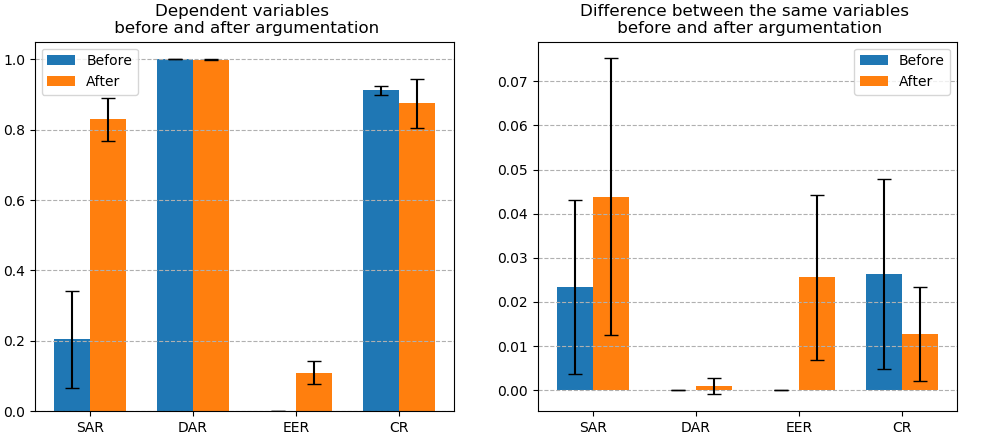
\includegraphics[width=\textwidth]{results/Figure_1_resized.png}
    \caption{}
    \label{fig:gen_intro}
\end{figure}

Figure \ref{fig:gen_intro} presents all the ratio that have been measured, before and after the argumentation. The most important are the SAR and the DAR, as the EER and the CR will be explored with more details in  future hypothesis tests. The leftmost figure presents the overall measures. The DAR, that is in essence a local measure which compares two contrast sets of a same agent, is here presented as the average of two DARs of the agents, averaged again over the 200 experiments. The rightmost figure presents the average difference between the local measures of a same experiment. Since the SAR, EER and CR are global measures, we propose a formulation for their local counterparts. The local SAR of an agent $A$ is computed by using the local context of $A$ instead of the overall context as the denominator of the ratio. The local EER of $A$ is computed by using the number of examples sent by $A$ as the numerator of the ratio, instead of using the number of examples exchanged by the two agents which would also include the number of examples received by $A$. Finally, the local CR of $A$ is computed by dividing the number of examples from $A$'s context that are covered by one of its current contrast set's concept, by the number of examples in $A$'s context.

We can see on the leftmost figure that the DAR of both agents is one both before and after the argumentation, meaning that the agents refined their respective contrast sets in a monotonic way, without compromising their original classifications. Moreover, the SAR significantly increases after the argumentation. The agents are therefore able to reach mutual intelligibility while refining their contrast sets in a monotonic way with our model. The EER stays around 0.1 with a low variance, meaning that the agents do not need to exchange more than $10\%$ of their examples to reach mutual intelligibility for any type of disagreement combination encountered. The CR decreases after the argumentation, meaning that less examples are covered after the argumentation. This is coherent with the fact that our model has been design to chose refinement over coverage. However, the difference between the CR before and after the argumentation is small, with a CR after argumentation well above 0.5, which indicates that the refinement does not cause an over-fitting.

The scale on the rightmost figure ranges from 0 to 0.08. This means that the difference between the local measures on the two agents ranges on a tenth of the global measures. From this, we can conclude that there is no asymmetry between the knowledge of our agents before or after the argumentation.

\subsection{Lazy Strategy}

%%% DOMAIN INDEPENDENCE
\section{Domain Independence}

The domain independence hypothesis postulates that both approaches of our model can resolve a disagreement between two agents that occurs on any domain, increasing the SAR of the agents while keeping their respective DAR at one. In order to test this hypothesis, we used with four different domains, and set up exactly \emph{one} overlap disagreement between two agents on each of them. Moreover, the examples that have not been used in the set up of the overlap are removed from the data set of the agents before the beginning of the argumentation, in order to ensure that we do not have more concepts that are not used in a set up in some domains than in others. We tested this experiment 100 times on and averaged the measures in order to present the results below. 

In each of the 100 experiments, the SAR, DAR, EEC and CR of the agents are measured in each of the four argumentation occurring on the different domains. The four domains are the independent variables our our experiment, while the SAR, DAR, EEC and CR are the dependent variables. The argument acceptability is 0.75, its standard value, and the redundancy is set at $0\%$ as usual. However, the error threshold is different for each data set. The error threshold is set in order to ensure that at least 3 classes from a set of classes of comparable sizes are available to set up the overlap in each data set. We decided on $\tau_{E} = 1$ for the Seat domain, $\tau_{E} = 6$ for the Zoology domain, $\tau_{E} = 10$ for the Sponges domain and $\tau_{E} = 11$ on the Soybean domain.

\subsection{Systematic Strategy}

\begin{figure}
    \centering
    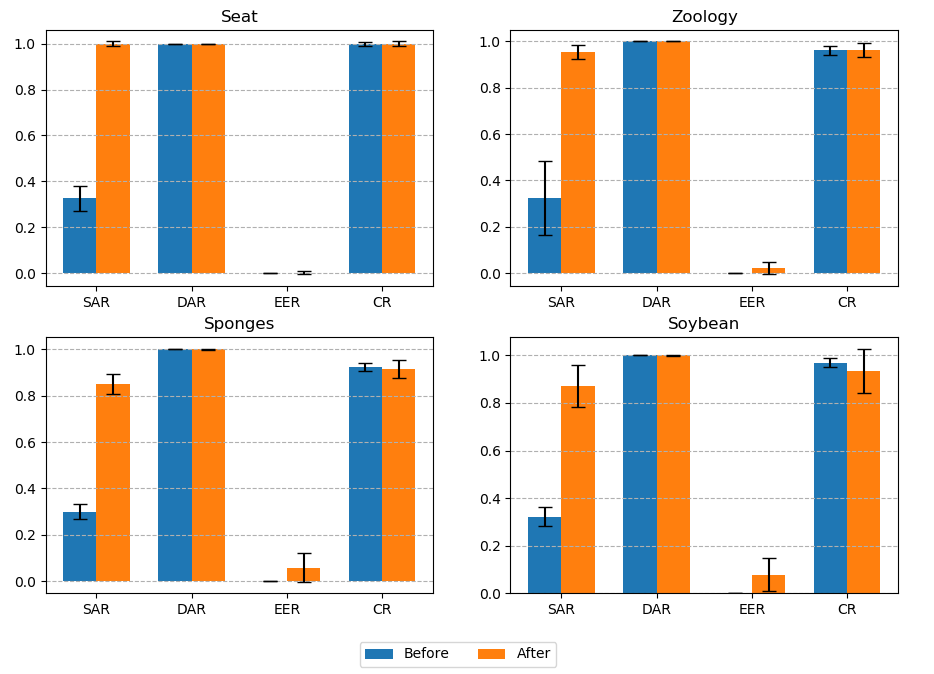
\includegraphics[width=\textwidth]{results/Figure_4_resized.png}
    \caption{Ratios measured before and after an argumentation, over the four different domains \emph{Seat}, \emph{Zoology}, \emph{Sponges} and \emph{Soybean}.}
    \label{fig:ind_intro}
\end{figure}

The results of this experiment are shown in Figure \ref{fig:ind_intro}. Each of the four sub-figures represents the four ratios measured on a specific domain, before and after the argumentation.
% SAR
We can observe a generalized increase of the SAR for all domains. The SAR before argumentation is on average at a predictable 0.33 for all domains, with a low variability except for the Zoology domain which is the domain where the distribution of the examples among the classes over $2 \times \tau_{E}$ elements is the most irregular. The average SAR after argumentation can vary from 0.83 to 1.0, depending on the domain. The systematic strategy achieves the highest increase of the SAR, with a final SAR of 1.0, meaning that the synchronic agreement is fully reached. The systematic strategy obtains a final SAR of 0.95 on average on the Zoology domain, and around 0.85 on the Sponges (0.85) and Soybean (0.87) domains. These results correlate with the complexity, in terms of different attributes, of the different domains.
% DAR
The DAR is maintained at 1 in every domain, with a standard deviation always close to 0. There is always a full diachronic agreement for both agents.

% EER
There are logically no example exchanged before the argumentation. The augmentations on the Seat domain are done without example exchanges, as the EER stays at 0 with a low standard deviation. On the other domains, the EER increases with the complexity of the domain expressed in terms of different attributes. Zoology accounts for the lowest non-zero EER, followed by Sponges and finally Soybean. The EER evolution is evaluated more in detail with the test of the preservation hypothesis.

% CR
The CRs before argumentation correlates on the complexity of the domain. The Seat domain has a CR at 1 with low standard deviation before the argumentation, the Zoology domain has a CR at 0.96, the Sponges has a CR at 0.92 and the Soybean has a CR at 0.97. The CR stays constant for the Seat and the Zoology domain. However, it decreases significantly for the Sponges add the Soybean domains, the decrease being more pronounced in the case of the Soybean domain. The decreases are again correlated to the complexity of the domains, however the final CR always stay close to the value it had before the argumentation. Even after the argumentation, every CR stays above 0.9, leaving the agents with less than $10\%$ of their overall context unclassified on average.

Overall, the performances of our model are high for every domain. The SAR is the most impacted measure by increments in the domain's complexity, with a lowest final SAR at 0.85 in the case of the Sponges domain and a highest final SAR at 1. The average final SAR being at 0.87 for the Soybean domain in this experiment, while it was at 0.83 in the last experiment, leads us to think that the average SAR measured in a situation of set up overlap is a good indicator of the SAR that should be expected for a combination of set up disagreements. The DAR remains at 1, proving once again to be the most stable measure.

\subsection{Lazy Strategy}

\section{Coverage Preservation}

The preservation hypothesis postulates that most of the examples that were covered by a concept continue to be covered by another concept in the refined contrast set. While a diachronic agreement ensures that no pair of examples from the same extensional definition \emph{of the new context} was separated in the initial contrast set, the diachronic agreement does not constraint the new context to be a super-set of the initial context. Therefore, as our model often refines concepts, we can expect that a context after an argumentation is a subset of itself before the argumentation. In this sense, the hypothesis of preservation complements the respect of the diachronic agreement in making sure that after an argumentation, an agent can make equivalent classifications as before \emph{over the same context}.

The preservation hypothesis has already been partially explored during the experiments over the Generality and Domain Independence hypotheses. However, the measures were approximated. Indeed, the overall CR computed was each time obtained as the average between both local CRs. This approximation is only accurate if one local set of covered examples is a subset of the other. In this section, the preservation hypothesis will be correctly investigated by searching for the subset of examples from the overall context that are not covered by \emph{both} agents. In order to evaluate this hypothesis over different contexts, we repeated this experiment 100 times on each domain over which we observed a final CR inferior to 1 during the test of the domain independence hypothesis: Zoology, Sponges and Soybean.

% VI & VD
The independent variables of each experiment and their overall set up are similar to the independent variables and set up of the domain independence hypothesis test. One argumentation is set up using three random classes of the selected domain. The domain is the only independent variable. The parameters are the same as for the domain independence hypothesis test. The dependent variables are however different: the overall CR is the only dependent variable observed, and it is this the ratio of the examples from the overall context subsumed by the intensional definition of at least one concept of each agent, by the size of the overall context.

\subsection{Systematic Strategy}

\subsection{Lazy Strategy}

\section{Efficiency}

In order to reach an agreement, the agents could transfer their entire contexts to each others. The issues of finding the overall pairing relations from the local ones and of creating new concepts through argumentation would disappear. The remaining tasks for our agents would only be to define new extensional definitions, learn satisfying intensional definitions for them and elect at new lexicon for the resulting contrast set. An important part of our model is dedicated to circumvent the problems arising when they cannot transfer these examples. The efficiency hypothesis proposes that the mutual intelligibility is not reached by the agents exchanging such extensively their contexts. In order to test this hypothesis over different contexts, we repeated this experiment 100 times on each domain over which we observed a non-zero EER during the test of the domain independence hypothesis: Zoology, Sponges and Soybean. 

% VI and VD
The independent variables of this experiment, its overall set up and its parameters are the same as for the test of the domain independence hypothesis. The dependent variables measured are the final overall EER, the difference between the two final local EERs, and the ratio of the final EER, by the SAR.

\subsection{Systematic Strategy}

\subsection{Lazy Strategy}

\section{Scalability}

The efficiency hypothesis questioned the ability of our model to reach mutual intelligibility while exchanging a reasonable amount of examples. The scalability hypothesis is its counterpart with generalizations. While we expect our model to exchange a number of generalizations significantly higher than the number of examples exchanged, the efficiency hypothesis investigates the correlation between the number of generalizations exchanged and the size of the overall context. Our hypothesis is that if the number of generalizations exchanged increases polynomially with the size of the overall context, therefore our model should be computally efficient once the size of the overall context reaches a certain threshold.

In order to test this hypothesis, we tested our argumentation with overall contexts of increasing sizes over the Sponge data set. The Sponge data set offers the advantage to have a larger version which enumerates 280 sponges, classified in the same three different orders ranging from 68 to 117 sponges. Our agents have an argumentation over a selected proportion of these 280 sponges ranging from 120 to 280, with the class distribution remaining the same for each proportion. This experiment is repeated 100 in order to present average results.

% VI & VD

\subsection{Systematic Strategy}

\subsection{Lazy Strategy}

\section{Simplicity}

In the introduction, we explained the difficulty to differentiate between hidden overlapping concepts that should be created, and small overlaps due to the agent's underfitting initial learning. However, while setting up the experiments, the number of concepts in the initial data set is known with certitude. Comparing this initial number with the final number of concepts present in the contrast sets \emph{after} the argumentation on meaning allows us to see how many excessive concepts have been created during the argumentation. However, this measure would be imperfect in the sense that it would penalize our model for something it is not directly aiming to solve: the precision of the agent's initial learning. As the argumentation on meaning takes place after the initial learning, the measure of simplicity should take into account \emph{all} the overlaps between the two contrast sets' concepts, which corresponds to the polylexematic classes of the union of the two agents' left-paths associations. By counting these polylexematic classes that contain more examples than the error threshold, we obtain the number of expected concepts (NEC). Comparing the NEC with the NFC (number of final concepts) gives us a measure of the simplicity of our model.

Our hypothesis of simplicity is that the average difference between the NEC and the NFC is close to 0. A difference above 0 would mean that our model converges by creating more concepts than necessary, which should increase the costs of our argumentation model in term of example and generalization exchanges. A difference below 0 would mean that our model creates less concepts than necessary, which should decrease either the synchronic agreement ratio or the coverage ratio. In order to evaluate this hypothesis over different contexts, we repeated the Domain Independence experiment 100 times on each domain over which we observed a final CR inferior to 1 during the test of the domain independence hypothesis: Zoology, Sponges and Soybean. Each time, we calculated the NEC and the NFC, subtracting the former to the latter. 

\subsection{Systematic Strategy}

\subsection{Lazy Strategy}

\section{Paradigm Shift}

We rationally demonstrated in the introduction that our model operates in a different paradigm than the AMAIL algorithm it was initially based on. This hypothesis of a paradigm shift in our argumentation model is also tested empirically. In order to evaluate this hypothesis, we test our model 100 times in the same conditions as we did for the Generality hypothesis, but this time running the AMAIL algorithm using the set of left-path associations of the agents before and after an argumentation with our model. We then compare the SAR, DAR and CR obtains at the two different times for each run. If there is indeed a paradigm shift, we should observe either a poor SAR, DAR, CR or no termination of the AMAIL algorithm at all before our argumentation, and an improved SAR but decreased DAR after our argumentation. 

\subsection{Systematic Strategy}

%% We compare the number of concepts in the original data set with the expected concepts at the creation of the contrast sets and the number of of concepts in output

% The VI are the domain, the number of concepts in the original data-set and the error threshold

% The VD are the the expected concepts at the creation of the contrast sets and the number of of concepts in output

% We do the same with the lazy strategy
\subsection{Lazy Strategy}

\chapter{Discussion}\label{Discussion}
% Idea of discussion about the application of our PhD in a multi-level ontology
The main limitation of the thesis is that it does not present any grounding to the symbols: an argumentation to reach a mutual intelligibility over a given contrast set requires a prior agreement over the formulation language of our logical propositions that represent our examples and our generalizations (here, the feature term formalism).

% Problem with the recursivity of meaning
Each sort of this formalism can be seen as a particular contrast set, therefore we just moved the alignment problem one level lower in our ontology. Even by changing our formalism, we wouldn't be able to get rid of that problem -- because as long as we consider the language as a closed system of signs we encounter the "Wittgenstein" problem that everything is just a language game between our agents and there is no fix point, no base contrast set, that we can align without the a-priori of another contrast set alignment. This is the grounding problem.

% The meaning not as a classification but as a causation
However, it is possible to bypass this problem if we consider that what grounds the meaning is not a classification that should be shared by all agents (we would still fall in a recursive approach that leads to a dead end), but a measure of causation instead.

\chapter{Conclusion}\label{Conclusion}
\input{Chapters/Conclusion.tex}


\begin{appendices}
\chapter{Proofs}\label{Proofs}
\section{Proof of Theorem \ref{thm:Overall}}\label{proof:ThmOverall}
Given two concepts $C_{i}$ and $C_{j}$ that have for intensional definitions respectively $I_{i}$ and $I_{j}$, and two contexts $U_{1}$ and $U_{2}$, we are having the four adjunct sets: $Adj(I_{i},U_{1})$, $Adj(I_{i},U_{2})$, $Adj(I_{j},U_{1})$ and $Adj(I_{j},U_{2})$. Given an overall context $U_{O} = U_{1} \cup U_{2}$, we have also the two adjunct sets: $Adj(I_{i},U_{O})$ and $Adj(I_{j},U_{O})$. We will prove the validity of the \cref{thm:Overall}.

Let $A_{1}$ and $A_{2}$ be two semiotic agents, $A_{1}$ partitioning the context $U_{1}$ in the contrast set $K_{1} = \{ U_{1}, S_{1} \}$ and $A_{2}$ partitioning the context $U_{2}$ in the contrast set $K_{2} = \{ U_{2}, S_{2}\}$. Let $C_{i}$ and $C_{j}$ be two concepts such that $C_{i} \in S_{1}$ and $C_{j} \in S_{2}$. Let $C_{i} r_{K} C_{j}$ be the local pairing relation of the agent $A_{1}$ and $C_{i} r_{K'} C_{j}$ the local pairing relation of the agent $A_{2}$, and $C_{i} r_{O} C_{j}$ the overall pairing relation of $A_{1}$ and $A_{2}$ between $C_{i}$ and $C_{j}$.

\begin{lemma}\label{lemma:relative}
The relative complement of $Adj(I_{j},Ctn)$ in $Adj(I_{i},Ctn)$ satisfies $Adj(I_{i}, Ctn) - Adj(I_{j}, Ctn) = \{ e \in U_{Ctn} | I_{i} \sqsubseteq e \wedge I_{j} \not \sqsubseteq e  \}$.
\end{lemma}

\begin{proof}
Definition \ref{def:AdjI} states that for any intentional definition $I$ and container $Ctn$, $Adj(I,Ctn) = \{ e \in U_{Ctn} | I \sqsubseteq e \}$. Therefore, the relative complement of $Adj(I_{j},Ctn)$ in $Adj(I_{i},Ctn)$ is $Adj(I_{i}, Ctn) - Adj(I_{j}, Ctn) = \{ e \in U_{Ctn} | I_{i} \sqsubseteq e \wedge I_{j} \not \sqsubseteq e \}$.
\end{proof}

\begin{lemma}\label{lemma:relativeq}
The existence of an example $e \in U_{Ctn}$ such that $I_{i} \sqsubseteq e$ and $I_{j} \not \sqsubseteq e$ can be written $Adj(I_{i}, Ctn) - Adj(I_{j}, Ctn) \neq \emptyset$.
\end{lemma}

\begin{proof}
The existence of an example $e \in U$ such that an intensional definition $I \sqsubseteq e$ and another intensional definition $I' \not \sqsubseteq e$ can be written $\{ e \in U | I \sqsubseteq e \wedge I' \not \sqsubseteq e \} \neq \emptyset$. Since Lemma \ref{lemma:relative} states that $\{ e \in U_{Ctn} | I_{i} \sqsubseteq e \wedge I_{j} \not \sqsubseteq e \} \Leftrightarrow Adj(I_{i},Ctn)$ is $Adj(I_{i}, Ctn) - Adj(I_{j}, Ctn)$, then the existence of an example $e \in U_{Ctn}$ such that $I_{i} \sqsubseteq e$ and $I_{j} \not \sqsubseteq e$ can be written $Adj(I_{i}, Ctn) - Adj(I_{j}, Ctn) \neq \emptyset$
\end{proof}

\begin{lemma}\label{lemma:IC equivalence}
Let $C$ and $C'$ be two concepts that have as intentional definition respectively $I$ and $I'$. $Adj(C, Ctn) - Adj(C', Ctn)$ is equivalent to $Adj(I, Ctn) - Adj(I', Ctn)$.
\end{lemma}

\begin{proof}
Theorem \ref{thm:AdjSetEq} states that the adjunct set of a concept is the adjunct set of its intentional definition. Therefore, the set difference of the adjunct sets of two concepts is also the set difference of the adjunct sets of the intensional definitions of these two concepts.
\end{proof}

\begin{lemma}\label{lemma:sd11}
If $Adj(C_{i}, K_{1}) - Adj(C_{j}, K_{1})$ is not  empty, then $Adj(C_{i}, H_{O}) - Adj(C_{j}, H_{O})$ is also not empty.
\end{lemma}

\begin{proof}
Let $e$ be an example such that $e \in U_{1}$ such that $I_{i} \sqsubseteq e$ and $I_{j} \not \sqsubseteq e$. If $e$ exists, according to Lemma \ref{lemma:relativeq} $Adj(I_{i}, K_{1}) - Adj(I_{j}, K_{1}) \neq \emptyset$ and according to Lemma \ref{lemma:IC equivalence}, $Adj(C_{i}, K_{1}) - Adj(C_{j}, K_{1}) \neq \emptyset$. However, if $e$ exists and since $U_{1} \subset U_{0}$, then $e \in U_{0}$ and therefore $Adj(C_{i}, H_{O}) - Adj(C_{j}, H_{O}) \neq \emptyset$. Therefore:

\begin{center}
$Adj(C_{i}, K_{1}) - Adj(C_{j}, K_{1}) \neq \emptyset \Rightarrow Adj(C_{i}, H_{O}) - Adj(C_{j}, H_{O}) \neq \emptyset$
\end{center}
\end{proof}

\begin{lemma}\label{lemma:sd12}
If $Adj(C_{i}, K_{2}) - Adj(C_{j}, K_{2})$ is not empty, then $Adj(C_{i}, H_{O}) - Adj(C_{j}, H_{O})$ is also not empty.
\end{lemma}

\begin{proof}
Let $e$ be an example such that $e \in U_{2}$ such that $I_{i} \sqsubseteq e$ and $I_{j} \not \sqsubseteq e$. If $e$ exists, according to Lemma \ref{lemma:relativeq} $Adj(I_{i}, K_{2}) - Adj(I_{j}, K_{2}) \neq \emptyset$ and according to Lemma \ref{lemma:IC equivalence}, $Adj(C_{i}, K_{1}) - Adj(C_{j}, K_{2}) \neq \emptyset$. However, if $e$ exists and since $U_{2} \subset U_{0}$, then $e \in U_{0}$ and therefore $Adj(C_{i}, H_{O}) - Adj(C_{j}, H_{O}) \neq \emptyset$. Therefore:

\begin{center}
$Adj(C_{i}, K_{2}) - Adj(C_{j}, K_{2}) \neq \emptyset \Rightarrow Adj(C_{i}, H_{O}) - Adj(C_{j}, H_{O}) \neq \emptyset$
\end{center}
\end{proof}

\begin{lemma}\label{lemma:sd1}
If $Adj(C_{i}, K_{1}) - Adj(C_{j}, K_{1})$ is not  empty or $Adj(C_{i}, K_{2}) - Adj(C_{j}, K_{2})$ is not empty, then$Adj(C_{i}, H_{O}) - Adj(C_{j}, H_{O})$ is also not empty.
\end{lemma}

\begin{proof}
We know that $Adj(C_{i}, K_{1}) - Adj(C_{j}, K_{1}) \neq \emptyset \Rightarrow Adj(C_{i}, H_{O}) - Adj(C_{j}, H_{O}) \neq \emptyset$ (Lemma \ref{lemma:sd11}).
We know that $Adj(C_{i}, K_{2}) - Adj(C_{j}, K_{2}) \neq \emptyset \Rightarrow Adj(C_{i}, H_{O}) - Adj(C_{j}, H_{O}) \neq \emptyset$ (Lemma \ref{lemma:sd12}).
Therefore:

\begin{center}
$(Adj(C_{i}, K_{1}) - Adj(C_{j}, K_{1}) \neq \emptyset \vee Adj(C_{i}, K_{2}) - Adj(C_{j}, K_{2}) \neq \emptyset) \Rightarrow Adj(C_{i}, H_{O}) - Adj(C_{j}, H_{O}) \neq \emptyset$.
\end{center}
\end{proof}

\begin{lemma}\label{lemma:sd2}
If $Adj(C_{i}, H_{O}) - Adj(C_{j}, H_{O})$ is not empty, then either $Adj(C_{i}, K_{1}) - Adj(C_{j}, K_{1})$ is not empty or $Adj(C_{i}, K_{2}) - Adj(C_{j}, K_{2})$ is not empty.
\end{lemma}

\begin{proof}
For all $e_{x} \in U_{O}$, since $U_{O} = U_{1} \cup U_{2}$ then $e_{x} \in U_{1} \vee e_{x} \in U_{2}$. Therefore, if $\exists e \in U_{O}$ such that $I_{i} \sqsubseteq e$ and $I_{j} \not \sqsubseteq e$, then $e \in U_{1} \vee e \in U_{2}$. Therefore, according to Lemma \ref{lemma:relativeq}, we can write

\begin{center}
$Adj(C_{i}, H_{O}) - Adj(C_{j}, H_{O}) \neq \emptyset \Rightarrow (Adj(C_{i}, K_{1}) - Adj(C_{j}, K_{1}) \neq \emptyset \vee Adj(C_{i}, K_{2}) - Adj(C_{j}, K_{2}) \neq \emptyset)$.
\end{center}
\end{proof}

\begin{lemma}\label{lemma:sd}
$Adj(C_{i}, H_{O}) - Adj(C_{j}, H_{O})$ is not empty if and only if $Adj(C_{i}, K_{1}) - Adj(C_{j}, K_{1})$ is not empty or the set difference $Adj(C_{i}, K_{2}) - Adj(C_{j}, K_{2})$ is not empty.
\end{lemma}

\begin{proof}
We know that $(Adj(C_{i}, K_{1}) - Adj(C_{j}, K_{1}) \neq \emptyset \vee Adj(C_{i}, K_{2}) - Adj(C_{j}, K_{2}) \neq \emptyset) \Rightarrow Adj(C_{i}, H_{O}) - Adj(C_{j}, H_{O}) \neq \emptyset$ (Lemma \ref{lemma:sd1}).
We know that $Adj(C_{i}, H_{O}) - Adj(C_{j}, H_{O}) \neq \emptyset \Rightarrow (Adj(C_{i}, K_{1}) - Adj(C_{j}, K_{1}) \neq \emptyset \vee Adj(C_{i}, K_{2}) - Adj(C_{j}, K_{2}) \neq \emptyset)$ (Lemma \ref{lemma:sd2}). Therefore, since $(A \Rightarrow B) \wedge (B \Rightarrow A)$ is equivalent to $A \Leftrightarrow B$, we can write:

\begin{center}
$Adj(C_{i}, H_{O}) - Adj(C_{j}, H_{O}) \neq \emptyset \Leftrightarrow (Adj(C_{i}, K_{1}) - Adj(C_{j}, K_{1}) \neq \emptyset \vee Adj(C_{i}, K_{2}) - Adj(C_{j}, K_{2}) \neq \emptyset)$
\end{center}
\end{proof}

\begin{lemma}\label{lemma:SD}
$Adj(C_{i}, H_{O}) - Adj(C_{j}, H_{O})$ is empty if and only if the  $Adj(C_{i}, K_{1}) - Adj(C_{j}, K_{1})$ is empty and $Adj(C_{i}, K_{2}) - Adj(C_{j}, K_{2})$ is empty.
\end{lemma}

\begin{proof}
We know that $Adj(C_{i}, H_{O}) - Adj(C_{j}, H_{O}) \neq \emptyset \Leftrightarrow (Adj(C_{i}, K_{1}) - Adj(C_{j}, K_{1}) \neq \emptyset \vee Adj(C_{i}, K_{2}) - Adj(C_{j}, K_{2}) \neq \emptyset)$ (Lemma \ref{lemma:sd}).
We also know that, by definition, $\overbar{A - B \neq \emptyset}$ is $A - B = \emptyset$.
Also by definition, $\overbar{A \vee B} = A \wedge B$.
Therefore:

\begin{align*}
Adj(C_{i}, H_{O}) - Adj(C_{j}, H_{O}) = \emptyset &\Leftrightarrow \overbar{Adj(C_{i}, H_{O}) - Adj(C_{j}, H_{O}) \neq \emptyset}\\
&\Leftrightarrow \overbar{(Adj(C_{i}, K_{1}) - Adj(C_{j}, K_{1}) \neq \emptyset \vee Adj(C_{i}, K_{2}) - Adj(C_{j}, K_{2}) \neq \emptyset)}\\
&\Leftrightarrow (Adj(C_{i}, K_{1}) - Adj(C_{j}, K_{1}) = \emptyset \wedge Adj(C_{i}, K_{2}) - Adj(C_{j}, K_{2}) = \emptyset)
\end{align*}
\end{proof}

\begin{lemma}\label{lemma:intersection}
The intersection of $Adj(I_{j},Ctn)$ and $Adj(I_{i},Ctn)$ satisfies $Adj(I_{i}, Ctn) \cap Adj(I_{j}, Ctn) = \{ e \in U_{Ctn} | I_{i} \sqsubseteq e \wedge I_{j} \sqsubseteq e  \}$.
\end{lemma}

\begin{proof}
Definition \ref{def:AdjI} states that for any intentional definition $I$ and container $Ctn$, $Adj(I,Ctn) = \{ e \in U_{Ctn} | I \sqsubseteq e \}$. Therefore, the intersection of $Adj(I_{j},Ctn)$ in $Adj(I_{i},Ctn)$ is $Adj(I_{i}, Ctn) \cap Adj(I_{j}, Ctn) = \{ e \in U_{Ctn} | I_{i} \sqsubseteq e | I_{j} \sqsubseteq e \}$.
\end{proof}

\begin{lemma}\label{lemma:intersectionq}
The existence of an example $e \in U_{Ctn}$ such that $I_{i} \sqsubseteq e$ and $I_{j} \sqsubseteq e$ can be written $Adj(I_{i}, Ctn) \cap Adj(I_{j}, Ctn) \neq \emptyset$.
\end{lemma}

\begin{proof}
The existence of an example $e \in U$ such that an intensional definition $I \sqsubseteq e$ and another intensional definition $I' \sqsubseteq e$ can be written $\{ e \in U | I \sqsubseteq e \wedge I' \sqsubseteq e \} \neq \emptyset$. Since Lemma \ref{lemma:intersection} states that $\{ e \in U_{Ctn} | I_{i} \sqsubseteq e \wedge I_{j} \sqsubseteq e \} \Leftrightarrow Adj(I_{i},Ctn)$ is $Adj(I_{i}, Ctn) \cap Adj(I_{j}, Ctn)$, then the existence of an example $e \in U_{Ctn}$ such that $I_{i} \sqsubseteq e$ and $I_{j} \sqsubseteq e$ can be written $Adj(I_{i}, Ctn) \cap Adj(I_{j}, Ctn) \neq \emptyset$
\end{proof}

\begin{lemma}\label{lemma:IC equivalence2}
Let $C$ and $C'$ be two concepts that have as intentional definition respectively $I$ and $I'$. $Adj(C, Ctn) \cap Adj(C', Ctn)$ is equivalent to $Adj(I, Ctn) \cap Adj(I', Ctn)$.
\end{lemma}

\begin{proof}
see \ref{lemma:IC equivalence}
\end{proof}

\begin{lemma}\label{lemma:inter11}
If $Adj(C_{i}, K_{1}) \cap Adj(C_{j}, K_{1})$ is not  empty, then $Adj(C_{i}, H_{O}) \cap Adj(C_{j}, H_{O})$ is also not empty.
\end{lemma}

\begin{proof}
Let $e$ be an example such that $e \in U_{1}$ such that $I_{i} \sqsubseteq e$ and $I_{j} \sqsubseteq e$. If $e$ exists, according to Lemma \ref{lemma:intersectionq} $Adj(I_{i}, K_{1}) \cap Adj(I_{j}, K_{1}) \neq \emptyset$ and according to Lemma \ref{lemma:IC equivalence2}, $Adj(C_{i}, K_{1}) \cap Adj(C_{j}, K_{1}) \neq \emptyset$. However, if $e$ exists and since $U_{1} \subset U_{0}$, then $e \in U_{0}$ and therefore $Adj(C_{i}, H_{O}) \cap Adj(C_{j}, H_{O}) \neq \emptyset$. Therefore:

\begin{center}
$Adj(C_{i}, K_{1}) \cap Adj(C_{j}, K_{1}) \neq \emptyset \Rightarrow Adj(C_{i}, H_{O}) \cap Adj(C_{j}, H_{O}) \neq \emptyset$
\end{center}
\end{proof}

\begin{lemma}\label{lemma:inter12}
If $Adj(C_{i}, K_{2}) \cap Adj(C_{j}, K_{2})$ is not empty, then $Adj(C_{i}, H_{O}) \cap Adj(C_{j}, H_{O})$ is also not empty.
\end{lemma}

\begin{proof}
Let $e$ be an example such that $e \in U_{2}$ such that $I_{i} \sqsubseteq e$ and $I_{j} \sqsubseteq e$. If $e$ exists, according to Lemma \ref{lemma:intersectionq} $Adj(I_{i}, K_{2}) \cap Adj(I_{j}, K_{2}) \neq \emptyset$ and according to Lemma \ref{lemma:IC equivalence2}, $Adj(C_{i}, K_{1}) \cap Adj(C_{j}, K_{2}) \neq \emptyset$. However, if $e$ exists and since $U_{2} \subset U_{0}$, then $e \in U_{0}$ and therefore $Adj(C_{i}, H_{O}) \cap Adj(C_{j}, H_{O}) \neq \emptyset$. Therefore:

\begin{center}
$Adj(C_{i}, K_{2}) \cap Adj(C_{j}, K_{2}) \neq \emptyset \Rightarrow Adj(C_{i}, H_{O}) \cap Adj(C_{j}, H_{O}) \neq \emptyset$
\end{center}
\end{proof}

\begin{lemma}\label{lemma:inter1}
If $Adj(C_{i}, K_{1}) \cap Adj(C_{j}, K_{1})$ is not  empty or $Adj(C_{i}, K_{2}) \cap Adj(C_{j}, K_{2})$ is not empty, then $Adj(C_{i}, H_{O}) \cap Adj(C_{j}, H_{O})$ is also not empty.
\end{lemma}

\begin{proof}
We know that $Adj(C_{i}, K_{1}) \cap Adj(C_{j}, K_{1}) \neq \emptyset \Rightarrow Adj(C_{i}, H_{O}) \cap Adj(C_{j}, H_{O}) \neq \emptyset$ (Lemma \ref{lemma:inter11}).
We know that $Adj(C_{i}, K_{2}) \cap Adj(C_{j}, K_{2}) \neq \emptyset \Rightarrow Adj(C_{i}, H_{O}) \cap Adj(C_{j}, H_{O}) \neq \emptyset$ (Lemma \ref{lemma:inter12}).
Therefore:

\begin{center}
$(Adj(C_{i}, K_{1}) \cap Adj(C_{j}, K_{1}) \neq \emptyset \vee Adj(C_{i}, K_{2}) \cap Adj(C_{j}, K_{2}) \neq \emptyset) \Rightarrow Adj(C_{i}, H_{O}) \cap Adj(C_{j}, H_{O}) \neq \emptyset$.
\end{center}
\end{proof}

\begin{lemma}\label{lemma:inter2}
If $Adj(C_{i}, H_{O}) \cap Adj(C_{j}, H_{O})$ is not empty, then either $Adj(C_{i}, K_{1}) \cap Adj(C_{j}, K_{1})$ is not empty or $Adj(C_{i}, K_{2}) \cap Adj(C_{j}, K_{2})$ is not empty.
\end{lemma}

\begin{proof}
For all $e_{x} \in U_{O}$, since $U_{O} = U_{1} \cup U_{2}$ then $e_{x} \in U_{1} \vee e_{x} \in U_{2}$. Therefore, if $\exists e \in U_{O}$ such that $I_{i} \sqsubseteq e$ and $I_{j} \sqsubseteq e$, then $e \in U_{1} \vee e \in U_{2}$. Therefore, according to Lemma \ref{lemma:intersectionq}, we can write:

\begin{center}
$Adj(C_{i}, H_{O}) \cap Adj(C_{j}, H_{O}) \neq \emptyset \Rightarrow (Adj(C_{i}, K_{1}) \cap  Adj(C_{j}, K_{1}) \neq \emptyset \vee Adj(C_{i}, K_{2}) \cap Adj(C_{j}, K_{2}) \neq \emptyset)$.
\end{center}
\end{proof}

\begin{lemma}\label{lemma:inter}
$Adj(C_{i}, H_{O}) \cap Adj(C_{j}, H_{O})$ is not empty if and only if $Adj(C_{i}, K_{1}) \cap Adj(C_{j}, K_{1})$ is not empty or $Adj(C_{i}, K_{2}) \cap Adj(C_{j}, K_{2})$ is not empty.
\end{lemma}

\begin{proof}
We know that $(Adj(C_{i}, K_{1}) \cap Adj(C_{j}, K_{1}) \neq \emptyset \vee Adj(C_{i}, K_{2}) \cap Adj(C_{j}, K_{2}) \neq \emptyset) \Rightarrow Adj(C_{i}, H_{O}) \cap Adj(C_{j}, H_{O}) \neq \emptyset$ (Lemma \ref{lemma:inter1}).
We know that $Adj(C_{i}, H_{O}) \cap Adj(C_{j}, H_{O}) \neq \emptyset \Rightarrow (Adj(C_{i}, K_{1}) \cap Adj(C_{j}, K_{1}) \neq \emptyset \vee Adj(C_{i}, K_{2}) \cap Adj(C_{j}, K_{2}) \neq \emptyset)$ (Lemma \ref{lemma:inter2}). Therefore, since $(A \Rightarrow B) \wedge (B \Rightarrow A)$ is equivalent to $A \Leftrightarrow B$, we can write:

\begin{center}
$Adj(C_{i}, H_{O}) \cap Adj(C_{j}, H_{O}) \neq \emptyset \Leftrightarrow (Adj(C_{i}, K_{1}) \cap Adj(C_{j}, K_{1}) \neq \emptyset \vee Adj(C_{i}, K_{2}) \cap Adj(C_{j}, K_{2}) \neq \emptyset)$
\end{center}
\end{proof}

\begin{lemma}\label{lemma:Inter}
$Adj(C_{i}, H_{O}) \cap Adj(C_{j}, H_{O})$ is empty if and only if $Adj(C_{i}, K_{1}) \cap Adj(C_{j}, K_{1})$ is empty and $Adj(C_{i}, K_{2}) \cap Adj(C_{j}, K_{2})$ is empty.
\end{lemma}

\begin{proof}
We know that $Adj(C_{i}, H_{O}) \cap Adj(C_{j}, H_{O}) \neq \emptyset \Leftrightarrow (Adj(C_{i}, K_{1}) \cap Adj(C_{j}, K_{1}) \neq \emptyset \vee Adj(C_{i}, K_{2}) \cap Adj(C_{j}, K_{2}) \neq \emptyset)$ (Lemma \ref{lemma:inter}).
We also know that, by definition, $\overbar{A \cap B \neq \emptyset}$ is $A \cap B = \emptyset$.
Also by definition, $\overbar{A \vee B} = A \wedge B$.
Therefore:

\begin{align*}
Adj(C_{i}, H_{O}) \cap Adj(C_{j}, H_{O}) = \emptyset &\Leftrightarrow \overbar{Adj(C_{i}, H_{O}) \cap Adj(C_{j}, H_{O}) \neq \emptyset}\\
&\Leftrightarrow \overbar{(Adj(C_{i}, K_{1}) \cap Adj(C_{j}, K_{1}) \neq \emptyset \vee Adj(C_{i}, K_{2}) \cap Adj(C_{j}, K_{2}) \neq \emptyset)}\\
&\Leftrightarrow (Adj(C_{i}, K_{1}) \cap Adj(C_{j}, K_{1}) = \emptyset \wedge Adj(C_{i}, K_{2}) \cap Adj(C_{j}, K_{2}) = \emptyset)
\end{align*}
\end{proof}

We remind the definition of pairing partial set:

\pSet*

\begin{lemma}\label{lemma:U1}
$U_{0,C_{i},\overbar{C_{j}}}$ is empty if and only if $U_{1,C_{i},\overbar{C_{j}}}$ is empty and $U_{2,C_{i},\overbar{C_{j}}}$ is empty.
\end{lemma}

\begin{proof}
From lemma \ref{lemma:SD} we know that $Adj(C_{i}, U_{O}) - Adj(C_{j}, U_{O}) = \emptyset  \Leftrightarrow ( Adj(C_{i}, U_{1}) - Adj(C_{j}, U_{1}) = \emptyset  \wedge Adj(C_{i}, U_{2}) - Adj(C_{j}, U_{2}) = \emptyset )$ and therefore by Definition \ref{def:PSet} it holds that $U_{0,C_i,\overbar{C_j}} = \emptyset \Leftrightarrow  (U_{1,C_i,\overbar{C_j}} = \emptyset \wedge U_{2,C_i,\overbar{C_j}} = \emptyset)$
\end{proof}


\begin{lemma}\label{lemma:U2}
$U_{0,C_{i},C_{j}}$ is empty if and only if $U_{1,C_{i},C_{j}}$ is empty and $U_{2,C_{i},C_{j}}$ is empty.
\end{lemma}

\begin{proof}
From the lemma \ref{lemma:Inter} we know that $Adj(C_{i}, U_{O}) \cap Adj(C_{j}, U_{O}) = \emptyset  \Leftrightarrow (Adj(C_{i}, U_{1}) \cap Adj(C_{j}, U_{1}) = \emptyset \wedge Adj(C_{i}, U_{2}) \cap Adj(C_{j}, U_{2}) = \emptyset)$ and therefore by Definition \ref{def:PSet} it holds that $U_{0,C_i,C_j} \Leftrightarrow  (U_{1,C_i,C_j} = \emptyset \wedge U_{2,C_i,C_j} = \emptyset)$.
\end{proof}

\begin{lemma}\label{lemma:U3}
$U_{0,\overbar{C_{i}},C_{j}}$ is empty if and only if $U_{1,\overbar{C_{i}},C_{j}}$ is empty and $U_{2,\overbar{C_{i}},C_{j}}$ is empty.
\end{lemma}

\begin{proof}
From the lemma \ref{lemma:SD} we know that $Adj(C_{i}, U_{O}) - Adj(C_{j}, U_{O}) = \emptyset  \Leftrightarrow (Adj(C_{i}, U_{1}) - Adj(C_{j}, U_{1}) = \emptyset \wedge Adj(C_{i}, U_{2}) - Adj(C_{j}, U_{2}) = \emptyset)$. Switching the variables $i$ and $j$, this is equivalent to $Adj(C_{j}, U_{O}) - Adj(C_{i}, U_{O}) = \emptyset  \Leftrightarrow (Adj(C_{j}, U_{1}) - Adj(C_{i}, U_{1}) = \emptyset \wedge Adj(C_{j}, U_{2}) - Adj(C_{i}, U_{2}) = \emptyset)$. Therefore, by Definition \ref{def:PSet} it holds that $U_{0,\overbar{C_i},C_j} \Leftrightarrow  (U_{1,\overbar{C_i},C_j} = \emptyset \wedge U_{2,\overbar{C_i},C_j} = \emptyset)$
\end{proof}

The r-triplets $r(C_{i}, C_{j}, U_{O})$, $r(C_{i}, C_{j}, U_{1})$ and $r(C_{i},C_{j},U_{2})$ are defined by the values of the pairing partial sets as presented in the definition \ref{def:RTriplet} that we recall below:

\rTriplet* 

Moreover, the values of the pairing partial sets from local contexts are linked to the values of the pairing partial sets from the overall context as shown in the lemmas \ref{lemma:U1}, \ref{lemma:U2} and \ref{lemma:U3}, therefore it is possible to find the values of the triplet $r(C_{i}, C_{j}, U_{O})$ knowing the values of the triplets $r(C_{i}, C_{j}, U_{1})$ and $r(C_{i},C_{j},U_{2})$.

\begin{lemma}\label{lemma:b-1}
Considering the triplets $r(C_{i},C_{j},U_{1}) = (b_{-1}, b_{0}, b_{1})$ and $r(C_{i},C_{j},U_{2}) = (b_{-1}', b_{0}', b_{1}')$ and $r(C_{i}, C_{j}, U_{O}) = (b_{-1}'', b_{0}'', b_{1}'')$, $b_{-1}''$ is equal to 0 if and only if $b_{-1}$ and $b_{-1}'$ are equal to 0. $b_{-1}''$ is equal to 1 otherwise.
\end{lemma}

\begin{proof}
According to the definition \ref{def:RTriplet}, $b_{-1}'' = 0$ if and only if $U_{0,C_i,\overbar{C_j}} = \emptyset$. However, according to the lemma \ref{lemma:U1} $U_{0,C_i,\overbar{C_j}} = \emptyset$ if and only if $U_{1,C_i,\overbar{C_j}} = \emptyset$ and $U_{2,C_i,\overbar{C_j}} = \emptyset$. The definition \ref{def:RTriplet} states that $(U_{1,C_i,\overbar{C_j}} = \emptyset$ if and only if $b_{-1} = 0$ and $(U_{2,C_i,\overbar{C_j}} = \emptyset$ if and only if $b_{-1}' = 0$. Therefore, $b_{-1}'' = 0$ if and only if $b_{-1} = 0$ and $b_{-1}' = 0$.
\end{proof}

\begin{lemma}\label{lemma:b0}
Considering the triplets $r(C_{i},C_{j},U_{1}) = (b_{-1}, b_{0}, b_{1})$ and $r(C_{i},C_{j},U_{2}) = (b_{-1}', b_{0}', b_{1}')$ and $r(C_{i}, C_{j}, U_{O}) = (b_{-1}'', b_{0}'', b_{1}'')$, $b_{0}''$ is equal to 0 if and only $b_{0}$ and $b_{0}'$ are equal to 0. $b_{0}''$ is equal to 1 otherwise.
\end{lemma}

\begin{proof}
According to the definition \ref{def:RTriplet}, $b_{0}'' = 0$ if and only if $U_{0,C_i,C_{j}} = \emptyset$. However, according to the lemma \ref{lemma:U2} $U_{0,C_i,C_{j}} = \emptyset$ if and only if $(U_{1,C_i,C_{j}} = \emptyset$ and $U_{2,C_i,C_{j}} = \emptyset)$. The definition \ref{def:RTriplet} states that $(U_{1,C_i,C_{j}} = \emptyset$ if and only if $b_{0} = 0$ and $(U_{2,C_i,C_{j}} = \emptyset$ if and only if $b_{0}' = 0$. Therefore, $b_{0}'' = 0$ if and only if $b_{0} = 0$ and $b_{0}' = 0$.
\end{proof}

\begin{lemma}\label{lemma:b1}
Considering the triplets $r(C_{i},C_{j},U_{1}) = (b_{-1}, b_{0}, b_{1})$ and $r(C_{i},C_{j},U_{2}) = (b_{-1}', b_{0}', b_{1}')$ and $r(C_{i}, C_{j}, U_{O}) = (b_{-1}'', b_{0}'', b_{1}'')$, $b_{1}''$ is equal to 0 if and only $b_{1}$ and $b_{1}'$ are equal to 0. $b_{1}''$ is equal to 1 otherwise.
\end{lemma}

\begin{proof}
According to the definition \ref{def:RTriplet}, $b_{1}'' = 0$ if and only if $U_{0,\overbar{C_i},C_j} = \emptyset$. However, according to the lemma \ref{lemma:U3} $U_{0,\overbar{C_i},C_{j}} = \emptyset$ if and only if $(U_{1,\overbar{C_i},C_{j}} = \emptyset$ and $U_{2,\overbar{C_i},C_{j}} = \emptyset)$. The definition \ref{def:RTriplet} states that $(U_{1,\overbar{C_i},C_{j}} = \emptyset$ if and only if $b_{1} = 0$ and $(U_{2,\overbar{C_i},C_{j}} = \emptyset$ if and only if $b_{1}' = 0$. Therefore, $b_{1}'' = 0$ if and only if $b_{1} = 0$ and $b_{1}' = 0$.
\end{proof}

The precedent lemmas are enough to prove Theorem \ref{thm:Overall}, theorem that we recall below:

\Overall*

\begin{proof}
We can prove that $b_{-1}'' = 0$ if and only if $b_{-1} = 0$ and $b_{-1}' = 0$ (Lemma \ref{lemma:b-1}).
We can prove that $b_{0}'' = 0$ if and only if $b_{0} = 0$ and $b_{0}' = 0$ (Lemma \ref{lemma:b0}).
We can prove that $b_{1}'' = 0$ if and only if $b_{1} = 0$ and $b_{1}' = 0$ (Lemma \ref{lemma:b1}).
Therefore, for all $n \in \{-1, 0, 1\}$, the element of the overall triplet $b_{n}''=0$  if and only if $b_{n} = 0$ and $b_{n}' = 0$, and otherwise $b_{n}''=1$.
\end{proof}
\section{Proof of Property \ref{pp:ClassSetComb}}\label{proof:ClassSetComp}
Given two agents $A_{k}$ and $A_{-k}$. Given $I = \{ g_{1}, ..., g_{n} \}$ a set of generalizations, and $U_{O}$ the overall context of the agents, divided in two sets of example $U^{+}$ and $U^{-}$ that partition $U$. Given the belief $\alpha = \langle +, I, A_{-k} \rangle$:

\begin{lemma}

\end{lemma}
\section{Proof of Property \ref{pp:GArgSets}}\label{proof:GArgSets}
\input{Appendix/ProofGArgSet.tex}
\section{Proof of Property \ref{pp:gargumentFN}}\label{proof:FalseNeg}
Given two agents $A_{k}$ and $A_{-k}$. Given $I = \{ g_{1}, ..., g_{n} \}$ a set of generalizations, and $U_{O}$ the overall context of the agents, divided in two sets of example $U^{+}$ and $U^{-}$ that partition $U$. Given the belief $\alpha = \langle +, I, A_{-k} \rangle$:

\begin{lemma}\label{lm:FP1}
In term of binary relations, the set of $\alpha$'s false positive examples is $FP = \{ e \in U^{-} \cap U_{O} | I \sqsubseteq e \}$.
\end{lemma}

\begin{proof}
We stated in Section \ref{sec:BeliefCreate} that the set of negative elements of the belief $\alpha = \langle +, I, A_{-k} \rangle$ is $U^{-}$. We also stated that the set of positive assignments is  $\{ e \in U_{O} | I \sqsubseteq e \}$. Since the set of false positives is the intersection between the set of negative elements and the set of positive assignments, the set of false positives is $\{ e \in U^{-} \cap U_{O} | I \sqsubseteq e \}$.
\end{proof}

\begin{lemma}\label{lm:FP2}
In term of binary relations, the set of $\alpha$'s false positive examples is $FP = \{ e \in U^{-} | I \sqsubseteq e \}$.
\end{lemma}

\begin{proof}
We stated in Lemma \ref{lm:FP1} that the set of false positives is $\{ e \in U^{-} \cap U_{O} | I \sqsubseteq e \}$. Since $U^{+}$ and $U^{-}$ are partitioning $U_{O}$, $U^{-} \subset U_{O}$ and therefore $U_{O} \cap U^{-} = U^{-}$. Therefore, $FP = \{ e \in U^{-} | I \sqsubseteq e \}$.
\end{proof}

\begin{lemma}\label{lm:FN1}
In term of binary relations, the set of $\alpha$'s false positive examples is $FN = \{ e \in U^{+} \cap U_{O} | I \not \sqsubseteq e \}$.
\end{lemma}

\begin{proof}
We stated in Section \ref{sec:BeliefCreate} that the set of positive elements of the belief $\alpha = \langle +, I, A_{-k} \rangle$ is $U^{+}$. We also stated that the set of negative assignments is  $\{ e \in U_{O} | I \not\sqsubseteq e \}$. Since the set of false negatives is the intersection between the set of positive elements and the set of negative assignments, the set of false negatives is $\{ e \in U^{+} \cap U_{O} | I \not \sqsubseteq e \}$.
\end{proof}

\begin{lemma}\label{lm:FN2}
In term of binary relations, the set of $\alpha$'s false negative examples is $FN = \{ e \in U^{+} | I \not \sqsubseteq e \}$.
\end{lemma}

\begin{proof}
We stated in Lemma \ref{lm:FN1} that the set of false negatives is $\{ e \in U^{+} | I \not \sqsubseteq e \}$. Since $U^{+}$ and $U^{-}$ are partitioning $U_{O}$, $U^{+} \subset U_{O}$ and therefore $U_{O} \cap U^{+} = U^{+}$. Therefore, $FN = \{ e \in U^{+} | I \not \sqsubseteq e \}$.
\end{proof}

\begin{lemma}\label{lm:FPnUk}
The intersection between $FP$ and $U_{-k}$ is $FP \cap U_{-k} = \{e \in U^{-}_{-k} | I \sqsubseteq e \}$
\end{lemma}

\begin{proof}
According to Lemma \ref{lm:FP2}, $FP = \{ e \in U^{-} | I \sqsubseteq e \}$. By definition, $FP \cap U_{-k} = \{e \in (U^{-} \cap U_{-k}) | I \sqsubseteq e \}$. Moreover, in Section \ref{sec:funCreaConA}, we define $U^{-}_{k}$ as $U^{-} \cap U_{k}$. Therefore, $FP \cap U_{-k} = \{e \in U^{-}_{-k} | I \sqsubseteq e \}$.
\end{proof}

\begin{lemma}\label{lm:FPdisUo}
The local context $U_{-k}$ and the set of false positives $FP$ are disjoint.
\end{lemma}

\begin{proof}
We know from Lemma \ref{lm:FPnUk} that $FP \cap U_{-k} = \{e \in U^{-}_{-k} | I \sqsubseteq e \}$. However, according to Definition \ref{def:Belief}, $\nexists e \in U^{-}_{-k}$ such that $I \sqsubseteq e$. Therefore, $\{e \in U^{-}_{-k} | I \sqsubseteq e \} = \emptyset$ which means that $FP \cap U_{-k} = \emptyset$.
\end{proof}

\begin{lemma}\label{lm:FNnUk}
The intersection between $FN$ and $U^{+}_{-k}$ is $FN \cap U^{+}_{-k} = \{e \in U^{+}_{k} | I \not \sqsubseteq e \}$
\end{lemma}

\begin{proof}
According to Lemma \ref{lm:FN2}, $FN = \{ e \in U^{+} | I \not \sqsubseteq e \}$. By definition, $FN \cap U^{+}_{-k} = \{e \in (U^{+} \cap U_{k}) | I \not \sqsubseteq e \}$. Moreover, in Section \ref{sec:funCreaConA}, we define $U^{+}_{k}$ as $U^{+} \cap U_{k}$. Therefore, $FN \cap U^{+}_{-k} = \{e \in U^{+}_{k} | I \not \sqsubseteq e \}$.
\end{proof}

\begin{lemma}\label{lm:FNdisUo}
The local context $U_{-k}$ and the set of false negatives $FN$ are disjoint.
\end{lemma}

\begin{proof}
We know from Lemma \ref{lm:FNnUk} that $FN \cap U^{+}_{-k} = \{e \in U^{+}_{k} | I \not \sqsubseteq e \}$. However, according to Definition \ref{def:Belief}, we have $I \sqsubseteq U^{+}_{-k}$, which is equivalent to $\forall e \in U^{+}_{-k}, I \sqsubseteq e$. Therefore, $\{e \in U^{+}_{-k} | I \not \sqsubseteq e \} = \emptyset$ which means that $FN \cap U_{-k} = \emptyset$.
\end{proof}

Let $\gamma = \langle \alpha, x, I', A_{k} \rangle$ be a g-argument that attacks the belief $\alpha$. The positive examples of $\gamma$ are:

\begin{itemize}
    \item $P' = FN$ if $x$ is $+$
    \item $P' = FP$ if $x$ is $-$
\end{itemize}

\begin{lemma}\label{lm:FNx}
For any $x \in \{+,-\}$, the false negatives of the g-argument $\gamma$ are the examples $FN^{x} = \{ e \in (U_{O} \cap P') | I' \not\sqsubseteq e \}$.
\end{lemma}

\begin{proof}
By definition, the set of false negatives of $\gamma$ is the intersection between the set of positive examples of $\gamma$ which is $P'$, and the set of negative assignments of $\gamma$ which is $\{ e \in U_{O} | I' \not \sqsubseteq e \}$. Therefore, their intersection is $FN^{+} = \{ e \in (U_{O} \cap P') | I' \not\sqsubseteq e \}$
\end{proof}

\begin{lemma}\label{lm:FN+1}
If $x = +$, the false negatives of the g-argument $\gamma$ are the examples $FN^{+} = \{ e \in FN | I' \not\sqsubseteq e \}$.
\end{lemma}

\begin{proof}
Since $P' = FN$, and since $FN$ is a subset of $U_{O}$, $U_{O} \cap FN = FN$. Therefore, according to Lemma \ref{lm:FNx}, if $x$ is $+$, $FN^{+} = \{ e \in FN | I' \not\sqsubseteq e \}$.
\end{proof}

\begin{lemma}\label{lm:FN+2}
The set of examples $FN^{+} = \{ e \in FN | I' \not\sqsubseteq e \}$ is an empty set.
\end{lemma}

\begin{proof}
According to Lemma \ref{lm:FN+1}, if $x$ is $+$ then the set of $\gamma$'s false negatives is $FN^{+} = \{ e \in FN | I' \not\sqsubseteq e \}$.
\end{proof}

\begin{lemma}\label{lm:FN-1}
If $x$ is $-$, the false negatives of the g-argument $\gamma$ are the examples $FN^{-} \{ e \in FP | I' \not\sqsubseteq e \}$.
\end{lemma}

\begin{proof}
Since $P' = FP$, and since $FP$ is a subset of $U_{O}$, $U_{O} \cap FP = FP$. Therefore, according to Lemma \ref{lm:FNx}, if $x$ is $-$, $FN^{-} = \{ e \in FP | I' \not\sqsubseteq e \}$.
\end{proof}

\begin{lemma}\label{lm:FN-2}
The set of examples $FN^{-} = \{ e \in FP | I' \not\sqsubseteq e \}$ is an empty set.
\end{lemma}

\begin{lemma}
The g-argument $\gamma$ cannot have false negatives.
\end{lemma}

\begin{proof}
According to Lemma \ref{lm:FN+2}, the set of false negatives of $\gamma$ is empty if $x = +$. According to Lemma \ref{lm:FN-2}, the set of false negatives of $\gamma$ is empty if $x = -$. Since $x \in \{+,- \}$, the set of negative examples of a g-argument is always empty.
\end{proof}

\chapter{Evaluation of the Parameters}\label{apx:Parameters}
In Chapter \ref{Evaluations}, we briefly presented three parameters along with the usual independent and dependent variables. These three parameters of our model, redundancy, error threshold and argument acceptability are not tested as variables for two reasons: they are expected to impact the results in a predictable way, and they are two costly to test in terms of computation time to be extensively testes. However, the first of these two reasons is a hypothesis and, while we are not able to test it properly, we can give an overview of the reasons that led us to think that the redundancy, the error threshold and the argument acceptability have expected impacts on the results and which are these impacts. This is why the effects that variations of these parameters have on our model are tested below.

Instead of testing these parameters as variables during different augmentations, which would take a prohibitive amount of time, they are tested as variables over several different data sets in the creation of initial contrast sets. After the creation of the initial contrast sets, we can count the number of examples of each of the $2^{m+n}$ adjunct sets' intersections $Adj(i,U_{O}) \cup Adj(j,U_{O})$ for each pair of concepts $C_{i} \in K, C_{j} \in K'$ with $K$ having $m$ concepts and $K'$ having $n$ concepts. The number of intersections that have at least $\tau_{E}$ examples is the number of concepts that we should expect from a brute-force approach of the argumentation over the meaning.

The number of expected concepts is a good indicator of how the inductive learning of ABUI is going to perform over a given set of data, for a given degree of error and redundancy. The degree of error tolerated gives additional information on the values of $\tau_{E}$ that should be chosen in order to find a final number of concepts close to the number of categories of the data set used in the experiment.

We are testing these three parameters as variables over three different data sets: the zoology data set, the soybean data set and the sponges data set. We test the argument acceptability going from $0$ to $1.$, with an increasing step of $0.05$. The redundancy is tested on a range from $0 \%$ to $100 \%$, but with an increasing step of $50 \%$. However, we chose to let the number of examples in the initial contexts be the same regardless of the redundancy, for a given data set. In order to do so, the number of examples of each category $Ca$ in each agent's initial context is $|Ca|/2$. For instance, the category \emph{astrophorida} has 40 instances in the Sponges data set. Each agent will receive 20 examples from this category. If the redundancy is $100 \%$, they will receive the same subset of 20 astrophorida examples -- which still might be labeled differently. If we had distributed 21 examples, we could have still generated two different subsets of 21 examples that are $100 \%$ redundant; however, it would have been impossible to find two disjoint subsets of 21 astrophorida examples that are $0 \%$ redundant (there is less than $21 \times 2$ astrophorida examples in the Sponges data set).

The value of $\tau_{E}$, however, is not tested on the same range for all data sets. This is due to the fact that $\tau_{E}$ should be smaller than half of the examples of a certain amount of categories in order to allow the agents to find overall relations between their resulting concepts. For instance, if we set a $\tau_{E} = 20$ in an experiment that uses a data set where the largest category has $30$ examples, each agents will receive a set of $30/2 = 15$ examples of this category. Since $15 < \tau_{E}$, the pairing partial sets between the agents will always have a cardinal lower than $\tau_{E}$ and the agents will remain blind to the pairing relations between their concepts, thus forbidding an argumentation. For this reason, $\tau_{E}$ ranges from 0 to 5 for the Zoo data set, allowing to use the examples from 4 categories; $\tau_{E}$ ranges from 0 to 10 for the Soybean data set, allowing to use the examples from 6 categories and finally, $\tau_{E}$ ranges from 0 to 15 for the Sponges data set, allowing to use the examples from the 3 categories of the data set. On each of the data set, we test $\tau_{E}$ over the aforementioned range with an increasing step of 1.

\section{Impact of the parameters over inductive learning}

The experimental set-up of each instance of our three parameters' test is realized through the random selection of three different categories in the tested data set, that are merged differently for each agent in order to produce a scenario of expected overlap as it has been already presented in Chapter \ref{Examples}. Therefore, the number of expected concepts that we observe should always be compared to the three initial categories that have been used to set up the experiment. In an ideal case, we should observe three expected concepts: one for each involve category from the data set.

The overlap disagreement has the advantage to also produce two hypo-hypernymy disagreements, allowing us to have an expected initial situation with both types of semantic disagreements. We tested 10 times each combination of redundancy and argument acceptability for each of the three data sets, and presented the average number of expected concepts according to $\tau_{E}$ in Figure \ref{fig:param}. The results show that increasing the redundancy has a high impact on the number of expected concepts, which is easily understandable: by sharing more examples the agents can create generalizations that are as relevant in both contexts, thus explaining why the number of expected concepts converges to three - the number of involved categories from the data set - when the redundancy reaches $100 \%$. The results are presented in Figure \ref{fig:param}

\begin{figure}[t]
    \centering
    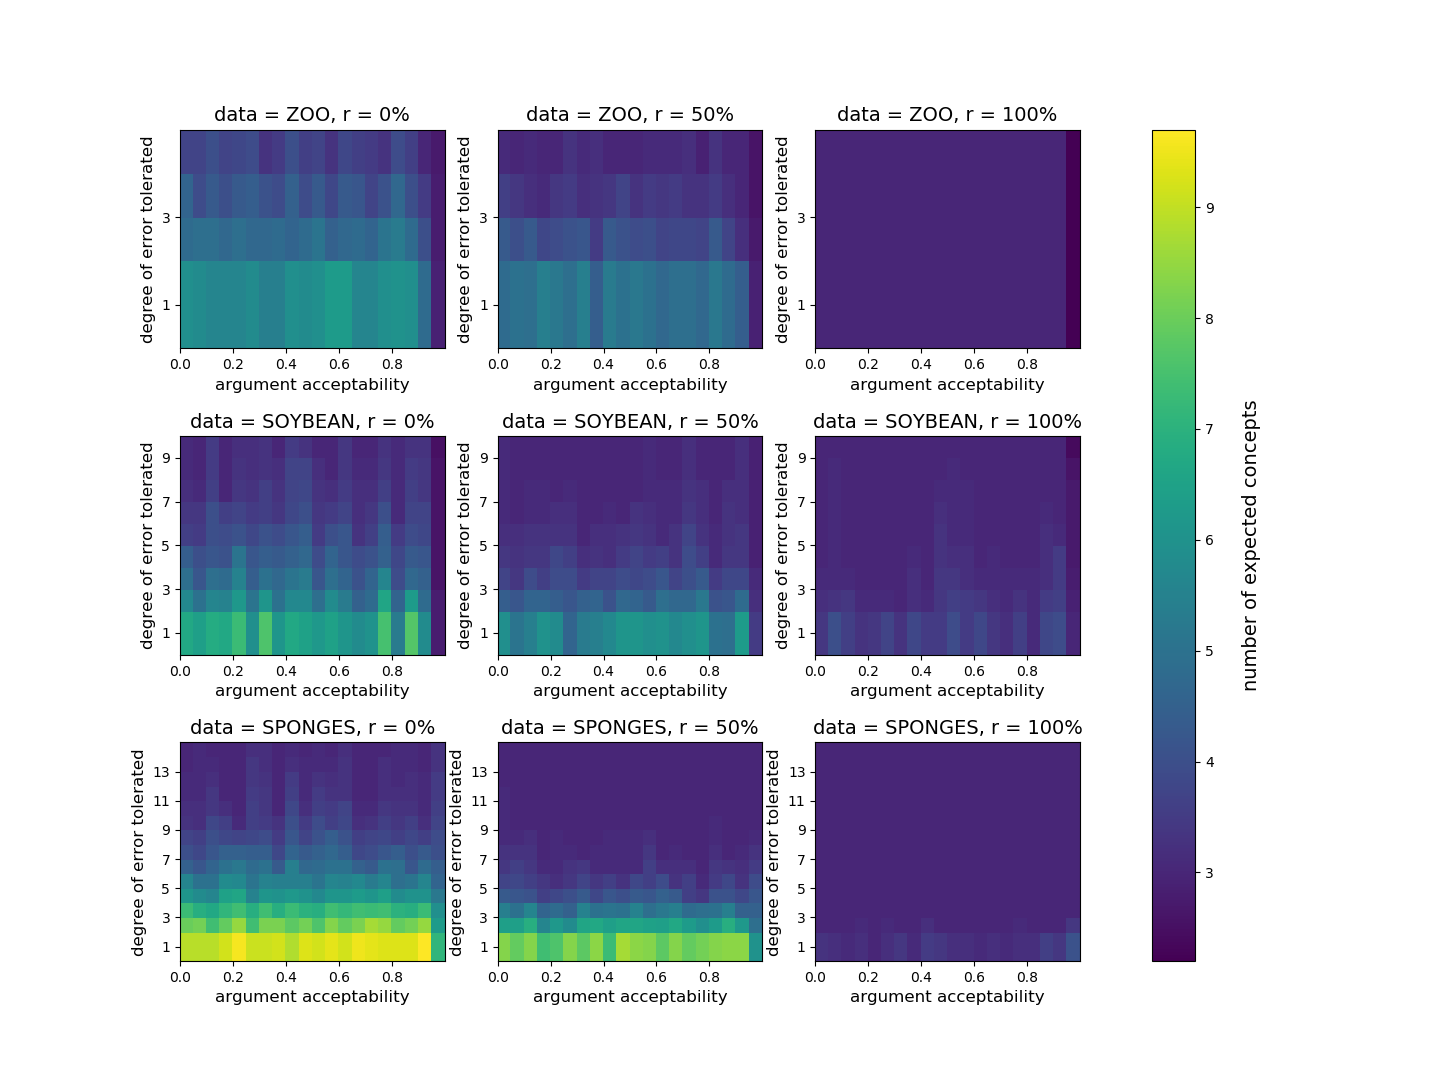
\includegraphics[width = \textwidth]{figs/Figure_parameters.png}
    \caption{Number of expected concepts for each combination of degree of error tolerated $\tau_{E}$, redundancy $r$ and argument acceptability, within the data sets Zoology (ZOO), Soybean (SOYBEAN) and Sponges (SPONGES).}
    \label{fig:param}
\end{figure}

The first thing to observe is that a low percentage of redundancy produces a number of expected concepts closer to three. If the agents start with the same examples in their contexts, they create generalizations that are more likely to correspond to the canonical cases already described in the Chapter \ref{Examples}. While this eases the argumentation, we want to test our argumentation protocol in the worst case of redundancy scenario and therefore, the redundancy parameter will always be set to $100 \%$ in our experiments

With a redundancy set at $100 \%$, we observe that the number of expected concepts depends mostly on the degree of error tolerated, regardless of the data set. With a low degree of error tolerated, we obtain too much concepts as the agents learn over-fit intensional definitions for their concepts. We clearly see that this issue peaks with the Sponges data set, where the number of expected concepts peaks over 9 for an error degree of 1. The lowest degree of error that provides consistently a number of expected concepts close to 3 depends on the data set observed: while $\tau_{E} = 5$ is already satisfying for the Zoology and the Soybean data set, $\tau_{E} = 8$ is a minimum for the Soybean data set.

\begin{figure}[t]
    \centering
    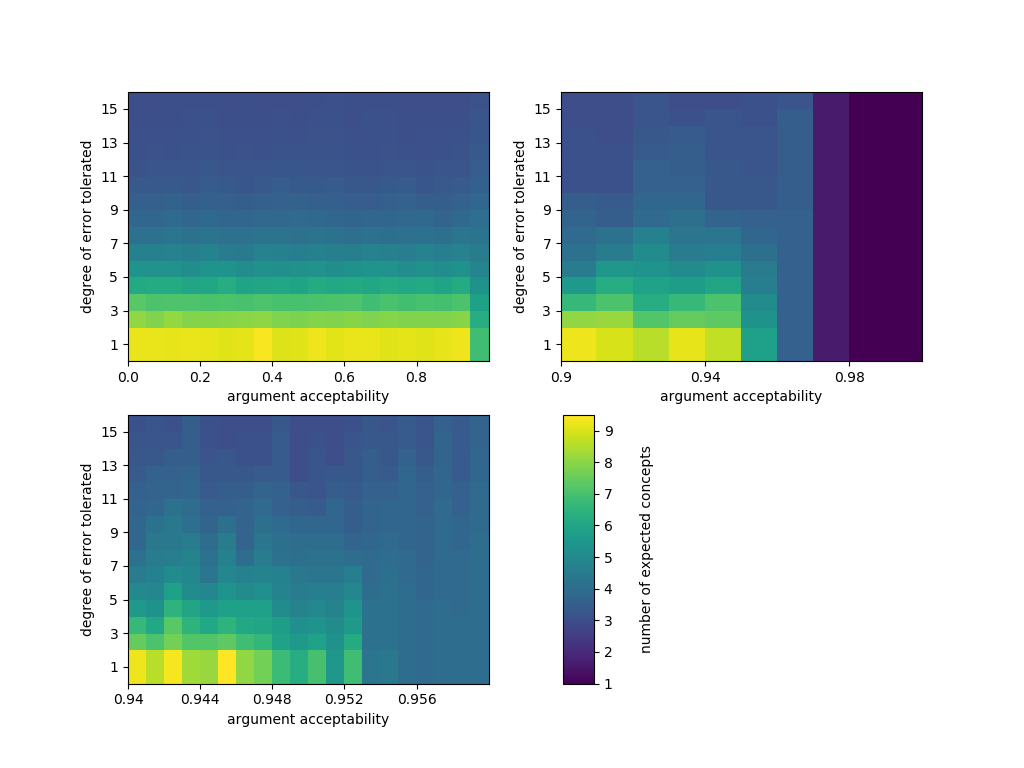
\includegraphics[width = \textwidth]{figs/Figure_AA.png}
    \caption{Impact of argument acceptability on the number of expected concepts on the Sponges data set and for a redundancy of $100\%$ between the two agents' data sets.}
    \label{fig:aa}
\end{figure}

Finally, the argument acceptability does not seems to impact the number of expected concepts, at the exception of its highest values. For each combination of data set, redundancy and degree of error, we can observe a constant number of expected concept until the argument acceptability reaches 0.95, where the number of expected concepts drops drastically, often to 0. The Figure \ref{fig:aa} presents the variation of the number of expected concepts with the sponges data set, for a redundancy of $100 \%$ and argument acceptability values close to 0.95. We can see that the argument acceptability does not influence the number of expected concepts under the value of 0.94. In our experiment, we chose an argument acceptability of 0.75 (? explain ABUI reasons), which is below this threshold.

\section{Impact of the error threshold over argumentation on meaning}

\begin{figure}[t]
    \centering
    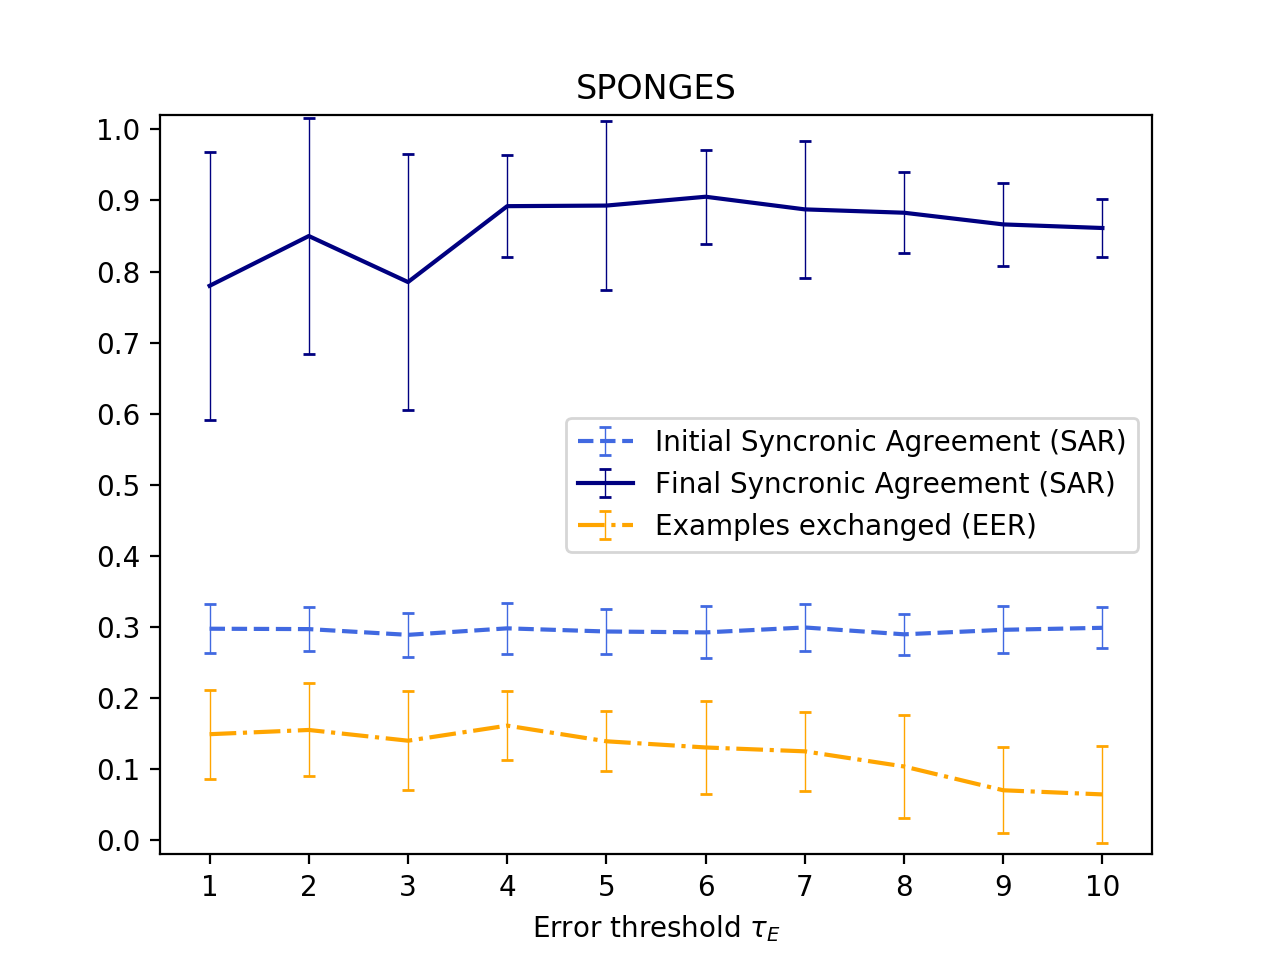
\includegraphics[width = \textwidth]{figs/threshold_SPON.png}
    \caption{Impact of the error threshold on synchronic agreement and examples exchanged, over an argumentation on overlaps in the Sponges data-set.}
    \label{fig:threshold_spon}
\end{figure}

After analyzing the different parameters of our experiments, we observed that the parameter which impacts the most the results of inductive learning is the error threshold. In order to evaluate the impact of the error threshold not only on inductive learning, but on a full argumentation, we are setting up a second experiment in which we measure three dependent variables: the initial synchronic agreement, the final synchronic agreement and the number of exchanged examples. The initial and final synchronic agreement are respectively measured at the beginning and the end of an experiment, using the Synchronic Agreement Ratio or SAR. The SAR is detailed in Section \ref{sec:variables}, and corresponds to the number of examples from the overall context that are named with the same unique sign by both agents divided by the total number of examples in the overall context. The number of exchanged examples is also measured as a ratio, corresponding to the number of examples that have been sent through messages by both agents divided by the total number of examples in the overall context.

The impact of error threshold is tested on two different data-sets: Sponges and Soybeans. For each data-set, we set the argument-acceptability to 0.75 and the redundancy to $0\%$. The error degrees tested vary from one to ten for the Sponges data-set, and from one to fifteen for the Soybean data-set. This difference is based on the comparative sizes of each data-set categories. The argumentation follows a systematic strategy over a setup of as many overlap as the threshold allows.Recall that in order to setup one overlap we need three categories of the data-set, and that in order to use a category of the data-set the number of examples in that category should not be lesser than twice the error threshold. This results in a major difference between the experiments on the two data-sets: while the Sponges data-set is limited to one overlap using any combination of its three 40-examples concepts regardless of the error threshold, the number of overlap increases as the error threshold decreases with the Soybeans data-set since the 19 categories have different numbers of concepts. The systematic strategy and the overlap setup are privileged as they correspond to a baseline setup: the lazy strategy is an adaptation of the systematic strategy, while the overlap setup creates two hypo/hypernymies and a synonymy as well, covering most of the disagreement cases.

\begin{figure}[t]
    \centering
    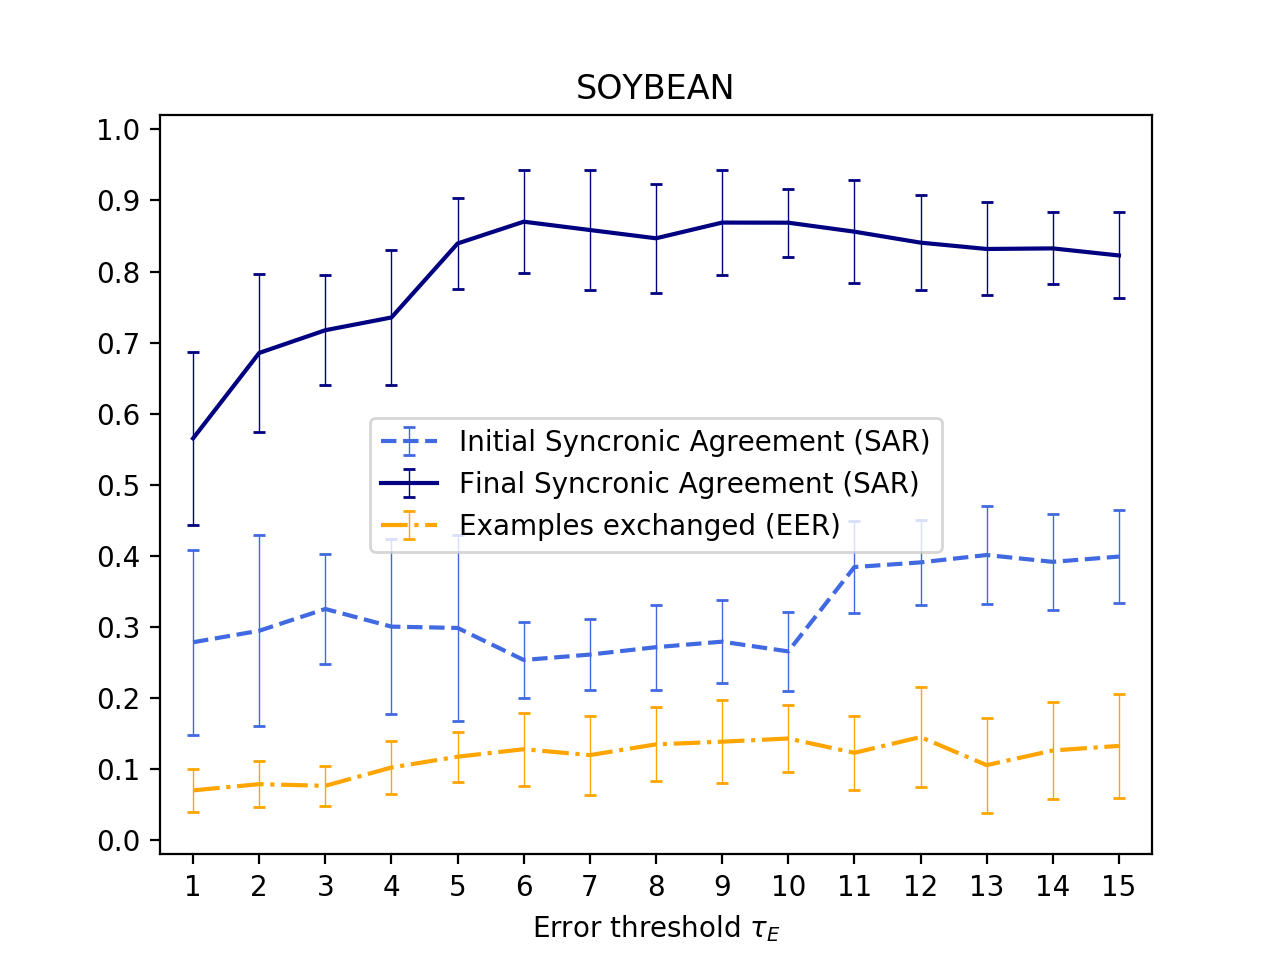
\includegraphics[width = \textwidth]{figs/threshold_SOY.png}
    \caption{Impact of the error threshold on synchronic agreement and examples exchanged, over an argumentation on overlaps in the Soybean data-set.}
    \label{fig:threshold_soy}
\end{figure}

For each data-set, we test the argumentation 500 times with a threshold randomly selected from the data-set dependent range presented in the previous paragraph. Figures \ref{fig:threshold_spon} and show, for each error threshold in absciss, the average initial and final synchronic agreement ratios and the average ratio of exchanged examples in ordinate, along with their standard deviations.

We observe that in both cases, the final synchronic agreement follows a same pattern: initially starting low with a great standard error, it stabilizes above 0.8 once the threshold reaches 5. However, the initial synchronic agreement has a significantly different profile for the two data-sets. With the sponges data-set, we observe an initial SAR that stays at stable to 0.3 regardless of the threshold with the Sponges data-set -- which is expected in a scenario of three concepts of the same size set up in an overlap, as it corresponds to one of the three initial concepts being the intersection of the two overlapping synonyms. On the contrary, the initial SAR in the Soybeans data-set displays multiple increasing and decreasing phases while the threshold varies, as the the threshold allows more or less classes of the data-set in the setup. For instance while we observe an initial SAR at 0.3 for a threshold ranging from 6 to 10, which corresponds to six usable concepts and therefore all of them involved in an overlap, the initial SAR rises at 0.4 above a threshold of 10 as only four concepts remains available for the overlap setup, three of them being used and the last one not causing significant disagreements to impact the initial SAR.

Finally, the number of examples exchanged is also impacted by the choice of the data-set. While the number of exchanged concepts decreases with the error threshold increasing in the Sponges data-set, it increases in the Soybean data-set -- although not by a lot, and mostly when the threshold increases from one to five. A good explanation for this are the poor performances of the argumentation for thresholds ranging on the same values: on that range, the final SAR is significantly below what it is for the same thresholds in the case of Sponges. The inability to generalize, thus not creating good intensional definitions for small concepts and stopping the argumentation early limits the exchange of examples.

\chapter{Messages}\label{apx:Messages}
This appendix lists the different types of content (Table \ref{tab:MessageContent}) and performatives (Table \ref{tab:Messageperformative}) that can be put in a message. 


\begin{table}
    \centering
    \begin{tabular}[t]{| >{\raggedright\arraybackslash}m{0.3\linewidth} | >{\raggedright\arraybackslash}m{0.3\linewidth}  | >{\raggedright\arraybackslash}m{0.3\linewidth} | } 
         \hline
         Class & Types & Notations \\
         \hline
         \hline
         Elementary Values & Boolean, Integer, Double & b, i, d \\
         \hline
         Semiotic Components & Examples, Generalizations & e, g \\
         \hline
         Semiotic Elements & Extensional Definition, Sign, Intensional Definition & $s$, $E$, $I$, $s(C)$, $E(C)$, $I(C)$ \\ 
         \hline
         Arguments & Root Arguments, Counter-Arguments & $\alpha$, $\beta$, \ldots \\ 
         \hline
         Identifiers & Concept Identifiers, Argument Identifiers & $i$, $i(C)$, $i(\alpha)$ \\
         \hline
         Evaluations & R-Triplets, Pairing Relations & $r(C_{i}, C_{j}, U)$, $(i_{-1}, i_{0}, i_{1})$, $C_{i} r_{U} C_{j}$, $\equiv$, $\odot$, $\oslash$, $\otimes$ \\
         \hline
    \end{tabular}
    \caption{Different types of content available for messages. The different types are regrouped by classes in the left column. The right column gives some examples of content in their canonical notation.}
    \label{tab:MessageContent}
\end{table}

\begin{table}
    \centering
    \begin{tabular}[t]{| >{\raggedright\arraybackslash}m{0.2\linewidth} | >{\raggedright\arraybackslash}m{0.25\linewidth}  | >{\raggedright\arraybackslash}m{0.45\linewidth} | } 
         \hline
         Performative & Content & Description \\
        \hline
        \hline
        Accept-Root, Accept-Argument & $i(\alpha)$ & Tells $A_{-k}$ that the argument $\alpha$ has been accepted by $A_{k}$'s standards.\\
        \hline
        Assert & $s(C)$, $i(C,A_{k})$, $I(C)$ & Informs the agent $A_{-k}$ that $A_{k}$ has a concept $C$, and shares its sign and intensional definition with $A_{-k}$.\\
        \hline
        Baptize & $s$ & Attributes a new sign $s$ to the concept that is currently being created. \\
        \hline
        Debate & $i(C_{i})$, $i(C_{j})$ & Proposes to resolve the disagreement caused by the relation between $C_{i}$ and $C_{j}$.\\
        \hline
        Examples & $E$ & Contains a set of examples $E$ for $A_{-k}$ to expends its local context.\\
        \hline
        Evaluation & $i(C_{i})$, $i(C_{j})$, $r(C_{i}, C_{j}, U)$ & Shares the r-triplet of $C_{i}$ and $C_{j}$ with $A_{-k}$.\\
        \hline
        Intransitive & $i(C_{1}), \ldots, i(C_{n})$ & Informs the agent $A_{-k}$ that from the point of view of $A_{k}$, $C_{1} \ldots C_{n}$ are breaking the transitivity rule of the equivalence pairing relation.\\
        \hline
        Name & $s$, $e$ & Tells $A_{-k}$ that $A_{k}$ associates the example $e$ with the sign $s$.\\
        \hline
        Relation & $i(C_{i})$, $i(C_{j})$, $r$ & Shares the pairing relation between $C_{i}$ and $C_{j}$ with $A_{-k}$.\\
        \hline
        Remove & $i(C_{1})$, $\ldots$, $i(C_{n})$ & Tells $A_{-k}$ that all instances of the concepts $i(C_{1})$, $\ldots$, $i(C_{n})$ should be removed from the argumentation.\\
        \hline
        Replace & $s$, $i(C)$ & Tells $A_{-k}$ that the sign of concept $C$ is now $s$.\\
        \hline
        Root-Argument, Counter-Argument & $\alpha$ & Sends an argument $\alpha$ to $A_{-k}$.\\
        \hline
        Seize & & Notifies $A_{-k}$ that $A_{k}$ will take care of an asymmetrical aspect of the argumentation during the next turn(s).\\
        \hline
        Self-Check & & Asks $A_{-k}$ to look for the pairing relations $R(S_{K,-k}, S_{H,-k}, U_{O})$.\\
        \hline
        Size & $i$ & Contains the size of a set of examples. Used to determine if a new concept has potentially enough examples to deserved to be created.\\
        \hline
        Vote & $s$, $i(C)$, $d$ & Gives a support of value $d$ to the fact that the concept $C$ should have $s$ for sign.\\
        \hline
    \end{tabular}
    \caption{The different performatives available for messages. Each performative (left column) is presented with the type of content that is expected to be found in its instances (middle column). The role of each performative is presented in the right column.}
    \label{tab:Messageperformative}
\end{table}
\end{appendices}

%------------------------------------------------------------------------------------------------------------------
% Bibliografia

\bibliographystyle{plain}
\bibliography{references.bib}

%------------------------------------------------------------------------------------------------------------------

%------------------------------------------------------------------------------------------------------------------
% Annex

\pagebreak
\thispagestyle{empty}

%------------------------------------------------------------------------------------------------------------------

\end{document}